\documentclass[aspectratio=149]{beamer}
\usetheme[compressed]{Singapore}
\usecolortheme{dove}
%\usetheme{Montpellier}
\useinnertheme{rounded}
\usepackage{graphicx}
\usepackage{setspace}
\usepackage{tikzsymbols}
\usepackage{longtable}
\usepackage{tabularx}
\usepackage[english]{babel}
\usepackage{tikzsymbols}
\usepackage{subcaption}
\usepackage{tikz}
\usepackage{spot}
\usepackage{tabularx}
\usepackage{booktabs}
\usepackage{tikzsymbols}
\usepackage{array,colortbl}
\usetikzlibrary{mindmap,calc,patterns,decorations.pathmorphing,decorations.markings, arrows, shapes.arrows, shapes, backgrounds,positioning,shadows.blur, positioning, fit, tikzmark, shadows}
\usepackage[absolute,overlay]{textpos}
\newcommand\Factor{1.2}
\setbeamerfont{subtitle}{family=\scshape}
\setbeamerfont{title}{family=\scshape}
%\definecolor{template}{RGB}{54, 114, 89}
\definecolor{template}{RGB}{155, 0, 20}
%\definecolor{background}{RGB}{250, 250, 250}
\definecolor{background}{RGB}{255, 255, 255}
\setbeamercolor{frametitle}{bg=background}
%\setbeamercolor{section in toc}{fg=template}
%\setbeamercolor{subsection in toc}{fg=black}
\setbeamerfont{section in toc}{size=\normalsize}
\setbeamertemplate{frametitle}{\color{black}\bfseries\scshape\insertframetitle\par\vskip2pt\hrulefill}
\setbeamercolor{section name}{fg=white}
\setbeamercolor{title}{fg=black, bg=background}
\setbeamercolor{section title}{fg=template}
\setbeamercolor{frame subtitle}{fg=template}
\setbeamercolor{title}{fg=black}
\setbeamercolor{background canvas}{bg=background}
\setbeamersize{text margin left=5mm,text margin right=5mm}
\setbeamercolor{section in head/foot}{bg=background, fg=black}
\setbeamercolor{subsection in head/foot}{fg=template, bg=template!20}
\usepackage[english]{babel}
\usepackage{tikz}
\usetikzlibrary{shapes.geometric, arrows}
\usepackage[absolute,overlay]{textpos}
\usepackage{graphicx}
\definecolor{myGreen}{RGB}{54, 114, 89}
\definecolor{repetition}{RGB}{58,95,205}
\definecolor{wp}{RGB}{197, 151, 0}
\definecolor{difference}{RGB}{181, 18, 27}
\definecolor{ic}{RGB}{106, 81, 163}
\setbeamercolor{item}{fg=myGreen!30}
%\setbeamersize{text margin left=3cm,text margin right=1.5cm} 
\AtBeginSection[]
{
	\begin{frame}
		\tableofcontents[currentsection]
	\end{frame}
}

\usepackage{tikz}
\usetikzlibrary{shapes.geometric, arrows}
\tikzstyle{startstop} = [rectangle, minimum width=1.5cm, minimum height=1cm,text centered, draw=black]
\tikzstyle{process} = [rectangle, rounded corners, minimum width=0.5cm, minimum height=1cm, text width =2.5cm, text centered, draw=black]
\tikzstyle{arrow} = [thick,->,>=stealth]

% rectangles on figures 
\newcommand{\imagenode}[2][1]% [scale], filename
{   \node[above right,inner sep=0] (myimage) {\includegraphics[scale=#1]{#2}};
	\path (myimage.north east);
	\pgfgetlastxy{\myimagex}{\myimagey}
	\pgfmathsetmacro{\myimagewidth}{\myimagex/28.453}
	\pgfmathsetmacro{\myimageheight}{\myimagey/28.453}
}
\newcommand{\imagegrid}[4][help lines]% [options], steps, font, precision
{   \pgfkeys{/pgf/number format/.cd,fixed,precision=#4}
	\foreach \x in {0,...,#2}
	{   \draw[#1] (\x/#2*\myimagewidth,\myimageheight) -- (\x/#2*\myimagewidth,0) node[below] {#3\pgfmathparse{\x/#2}\pgfmathprintnumber{\pgfmathresult}};
		\draw[#1] (\myimagewidth,\x/#2*\myimageheight) -- (0,\x/#2*\myimageheight) node[left] {#3\pgfmathparse{\x/#2}\pgfmathprintnumber{\pgfmathresult}};
	}
}

\newcommand{\highlightbox}[8][densely dashed,thick]% [options], left, low, right, up, node options, node text, overlay spec
{   \only<#8>{\draw[#1] (#2*\myimagewidth, #3*\myimageheight) rectangle node[#6] {#7} (#4*\myimagewidth, #5*\myimageheight);}
}

\newcommand{\highlighttext}[8][densely dashed,thick]% [options], left, low, right, up, node options, node text, overlay spec
{   \only<#8>{\path[#1] (#2*\myimagewidth, #3*\myimageheight) rectangle node[#6] {#7} (#4*\myimagewidth, #5*\myimageheight);}
}
%colonne 



\newenvironment{cols}[1][]{}{}

\newenvironment{col}[1]{\begin{minipage}{#1}\ignorespaces}{%
	\end{minipage}
	\ifhmode\unskip\fi
	\aftergroup\useignorespacesandallpars}

\def\useignorespacesandallpars#1\ignorespaces\fi{%
	#1\fi\ignorespacesandallpars}

\makeatletter
\def\ignorespacesandallpars{%
	\@ifnextchar\par
	{\expandafter\ignorespacesandallpars\@gobble}%
	{}%
}
\makeatother


\def\tikzoverlay{%
	\tikz[remember picture, overlay]\node[every overlay node]
}


%pop up
  \newcommand<>{\PutAt}[3][0pt]{%
	{\only#4{\begin{textblock*}{#1}#2%
				#3
	\end{textblock*}}}%
}
\newcommand<>{\NormalBox}[2][]{%
	\only#3{\tikz[#1, every node/.style={shape=rectangle,draw,fill=white, drop shadow, #1}]\node []{#2};}
}

% griglia pop up 
  \newcommand{\ShowPutAtGrid}{
	\begin{textblock*}{128mm}(0cm,0cm)
		\tikz[color=red!20!white]\draw[very thin, step=5mm] (0mm,0mm) grid (130mm,100mm);
	\end{textblock*}
	\begin{textblock*}{128mm}(0cm,0cm)
		\begin{tikzpicture}[color=red]
			\draw[step=1cm] (0,0mm) grid (130mm,100mm);   
			\foreach \n in {0,...,12}
			\draw[xshift=.5mm,yshift=-1.5mm, inner sep=0pt, anchor=west] (\n,10) node {\scriptsize{\textbf{\n}}};
			\foreach \n in {1,...,9}
			\draw[xshift=.5mm,yshift=-1.5mm, inner sep=0pt, anchor=west] (0,10-\n) node {\scriptsize{\textbf{\n}}};
		\end{tikzpicture}
	\end{textblock*}
}


\tikzset{type1/.style={circle, fill=blue},
	type2/.style={circle, fill=red},
	type3/.style={circle, fill=olive},
	type4/.style={circle, fill=cyan},
	type5/.style={circle, fill=giallo},
	type6/.style={circle, fill=blu},
	info/.style = {rectangle, rounded corners, minimum width=1.5cm, minimum height=10cm, text centered, draw=white,  text width=5.5cm},
	stat/.style = {rectangle, minimum width=1.5cm, minimum height=10cm, text justified, draw=white,  text width=5.5cm}
}

\usepackage[absolute,overlay]{textpos}

\renewcommand*{\thefootnote}{\fnsymbol{footnote}}


\tikzset{type1/.style={circle, fill=template},
	type2/.style={circle, fill=red},
	type3/.style={circle, fill=olive},
	type4/.style={circle, fill=cyan},
	type5/.style={circle, fill=giallo},
	type6/.style={circle, fill=template},
	info/.style = {rectangle, rounded corners, minimum width=2.5cm, minimum height=0.1cm, text centered, draw=black,  text width=2.5cm},
	stat/.style = {rectangle, rounded corners, minimum width=2.5cm, minimum height=0.1cm, text centered, draw=white,  text width=2.5cm}
}

%bordini colorati alle celle 

\def\highlight#1{%
	\fboxrule2pt %
	\hsize=\dimexpr\hsize-2\fboxrule-2\fboxsep\relax
	#1%
	\@endpbox\unskip\setbox0\lastbox\bgroup
	\fboxrule2pt %
	\fcolorbox{red}{lightgray}{\box0}\hfill}

\title{mat\texttt{R}iks}
\subtitle{An \texttt{R} package for the automatic generation of Raven-like matrices}
\author{Andrea Brancaccio, \textbf{Ottavia M. Epifania},  Debora de Chiusole, Pasquale Anselmi, Luca Stefanutti}
\date{Department of Philosophy, Sociology, Education and Applied Psychology, \\University of Padova, IT}
\institute [UniPd] {
	
\includegraphics[width=10mm]{img/unipd.png}\\ 
Dipartimento di Filosofia, Sociologia, Pedagogia e Psicologia Applicata,\\	Università di Padova}
	
	\date [AIP2023] {%\vspace{0.6cm}\\
		Convegno AIP-Sezione Sperimentale 2023\\Symposium: \\New frontiers for the adaptive assessment of executive functions\\ \vspace{3mm}
		18 Settembre 2023}
\begin{document}
	
\begin{frame}[plain]
    \maketitle
\end{frame}

\section{Introduction}

\begin{frame}

	Assessment of fluid intelligence or abstract reasoning 
	
	

	\begin{textblock*}{2cm}(9cm,1.5cm)
		
\includegraphics[width =\linewidth]{img/think2.png}
	\end{textblock*}
	
		\begin{textblock*}{2cm}(1.5cm,6.5cm)
		
\includegraphics[width =\linewidth]{img/think1.png}
	\end{textblock*}
	
	\vspace{5mm}
	Beyond clinical assessment $\rightarrow$ Job recruitment 
	
%	\pause
%	\begin{alertblock}{Issue}
%		
%%		\begin{itemize}
%Can only be administered once (or after a long time period)
%			
%	%		\item Difficulty in the generation of  ``true'' parallel forms
%	%	\end{itemize}
%	\end{alertblock}
%	
%	\pause
%	
%	\begin{exampleblock}{Aim}
%		
%		Development of an open-source easy-to-use tool for the automatic and  rule-based generation of Raven-like matrices
%	\end{exampleblock}
	
\end{frame}

\begin{frame}{An example}
	\centering
	\begin{tikzpicture}
		\imagenode[0.5]{img/completeExample.png}
		
		%     \imagegrid{10}{\tiny}{1}
		
		\highlightbox[red,very thick]{0.12}{0.49}{0.85}{0.98}{red}{}{2-3}
		\highlightbox[myGreen,very thick]{0.56}{0.50}{0.76}{.67}{myGreen}{}{3}
		\highlightbox[green,very thick]{0.03}{0.01}{0.98}{0.45}{red}{}{4}
	\end{tikzpicture}
	
\end{frame}


\begin{frame}{An example: The matrix}
	\centering
	\begin{tikzpicture}
		\imagenode[0.5]{img/matrix.png}
	%\imagegrid{10}{\tiny}{1}	
		\highlighttext{0.2}{0.9}{0.8}{1}{red}{Change shapes \& numerical progression}{2}
		\highlightbox[red,very thick]{0.18}{0.65}{0.85}{0.9}{red}{}{2}
		\highlightbox[red,very thick]{0.18}{0.37}{0.85}{0.62}{red}{}{2}
		\highlightbox[red,very thick]{0.18}{0.11}{0.85}{0.35}{red}{}{2}
		\highlightbox[red,very thick]{0.18}{0.1}{0.36}{0.9}{red}{}{3}
			\highlightbox[red,very thick]{0.40}{0.1}{0.60}{0.9}{red}{}{3}
		\highlightbox[red,very thick]{0.64}{0.1}{0.83}{0.9}{red}{}{3}
		\highlighttext{0.1}{0.9}{0.4}{1}{red}{Numerical progression}{3}
	\end{tikzpicture}
\end{frame}

\begin{frame}{An example: The response list}
	
\onslide<1->
	\begin{textblock*}{4cm}(8.5cm,1cm)
	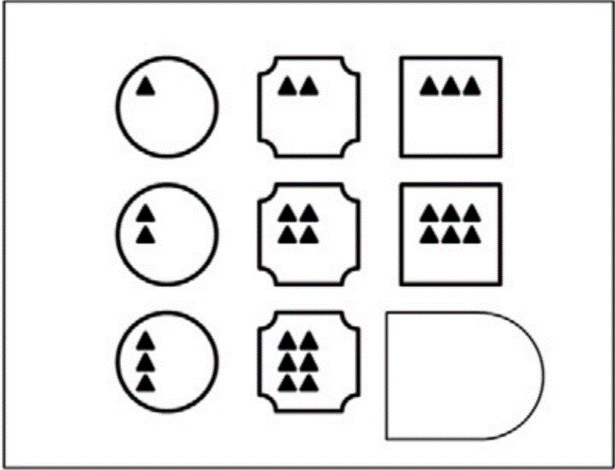
\includegraphics[width =\linewidth]{img/matrix.png}
\end{textblock*}


\begin{tikzpicture}
	\imagenode[0.4]{img/responses.png}
	\highlightbox[myGreen,very thick]{0.52}{0.02}{0.73}{.4}{circle,myGreen}{}{2-}
	\highlightbox[repetition,very thick]{0.52}{0.52}{0.73}{.86}{circle,myGreen}{}{3-}
	\highlightbox[repetition,very thick]{0.78}{0.02}{0.98}{.4}{circle,myGreen}{}{3-}
	\highlightbox[difference,very thick]{0.26}{0.52}{0.48}{.86}{circle,myGreen}{}{6-}
	\highlightbox[wp,very thick]{0.01}{0.02}{0.21}{.4}{circle,myGreen}{}{5-}
	\highlightbox[wp,very thick]{0.78}{0.52}{0.98}{.86}{circle,myGreen}{}{5-}
	\highlightbox[wp,very thick]{0.28}{0.02}{0.48}{.4}{circle,myGreen}{}{5-}
	\highlightbox[ic,very thick]{0.01}{0.52}{0.21}{.86}{circle,myGreen}{}{4-}
\end{tikzpicture}

\small 
\vspace{5mm}
	
	\onslide<3->
	\centering
	\scalebox{.95}{
		\begin{tabular}{p{3cm}p{10cm}}
		
		\textcolor<3->{repetition}{Repetition} &  Repetition of a cell adjacent to the blank space \\ 
				\textcolor<4->{ic}{Incomplete Correlate} &  Almost the correct response \\
						\textcolor<5->{wp}{Wrong Principle} &  Copy of a non adjacent cell or combination of cells \\
		\textcolor<6->{difference}{Difference} &  Different in appearance from every element of the matrix\\


		
		
	\end{tabular}
	}
	

	

\end{frame}

\section{Generating rules}

\begin{frame}
	\centering
	\scalebox{.60}{
	\begin{tabular}{p{2cm}p{4cm} p{8cm}}
		\hline
		Category	&	Rule name	&	Definition	\\
		\hline
		Visuospatial &	Object addition	&	Visually merge two objects 	\\
		&	Movement	&	Change the position of an object across the cells	\\
		&	Rotation	&	Change the spatial orientation of the objects across the cells	\\
		&	Mental transformation	& Apply the characteristics of the objects  in the second cell to the objects in the first cell to obtain the object in the third cell.	\\
		&	Numerical progression	&	Quantitative increase or decrease in the number of objects from cell to cell	\\
		&	Changes in shape	&	Change objects across cells 	\\
		&	Changes in shade	&	Change the shade of the objects across cells 	\\
		&	Changes in size	&Change the size of the objects across cells 	\\
		&	Changes in outline	&	Change the outline of the objects  across cells 	\\
		&&\\
		\hline
		Logical	&	AND	&	The third cell contains only the elements that appeared in both the first and second cells ($\cap$)	\\
		&	OR	&	The third cell contains all the elements in the first and second cells ($\cup$)	\\
		&	XOR	&	The third cell contains the elements in the first cell not present in the second cell and vice-versa ($\Delta$)	\\
		&&\\
		\hline
		Directional Logic & Horizontal & The objects are modified across columns \\
		& Vertical & The objects are modified across rows \\
		& Diagonal & The objects are modified horizontally and diagonally\\ \hline
	\end{tabular}}
\end{frame}

\section{The mat\texttt{R}iks package}

\begin{frame}
		\begin{textblock*}{2cm}(5.5cm,1cm)
		
\includegraphics[width =.7\linewidth]{img/github.png}
	\end{textblock*}
\begin{center}
	
	
	\small{	\texttt{devtools::install\_github("https://github.com/OttaviaE/matRiks")}}

\end{center}

		
	\begin{itemize}
		\item 	Generates $2 \times 2$ or $3 \times 3$ Raven-like matrices
		
		
	\item 	Generates the response list associated with the matrix (1 correct response $+$ 10 distractors)
	
	\item Core elements: 
	
	\vspace{3mm}
	\begin{quote}
		\textcolor<2->{myGreen}{Objects} \hspace{2mm} \textcolor<2->{myGreen}{Rules} \hspace{2mm} \textcolor<3->{template}{Matrix generator} \hspace{2mm} \textcolor<3->{template}{Response options generator}
	\end{quote}
	\end{itemize}

	
	
\end{frame}

\begin{frame}{(Some) of the available objects}
	\centering
	
	
	\begin{tabular}{c c c c}
		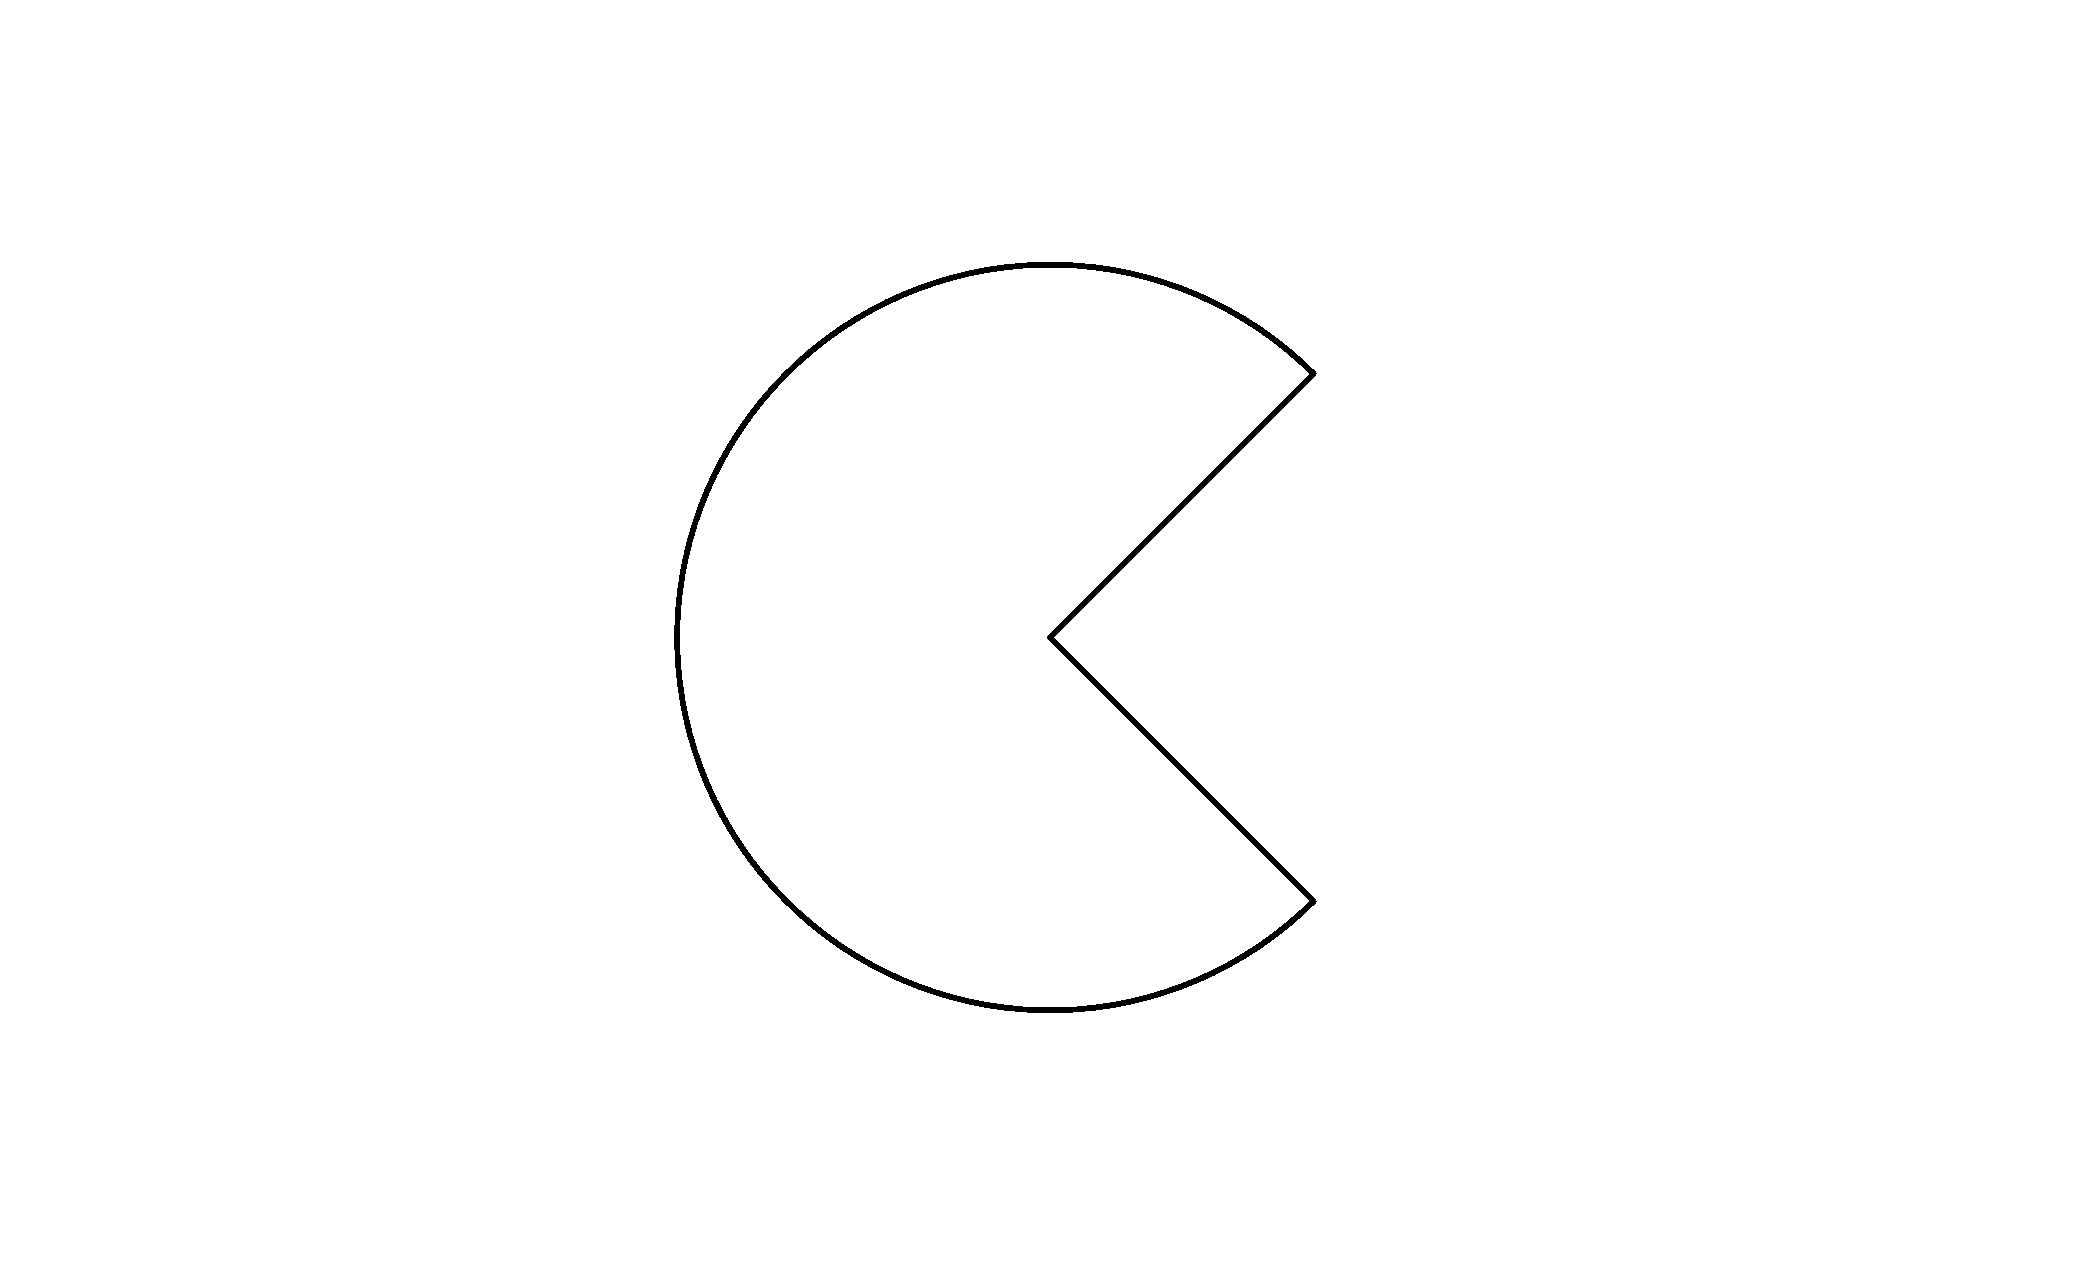
\includegraphics[width=0.2\linewidth]{img/pacman.pdf} & 
		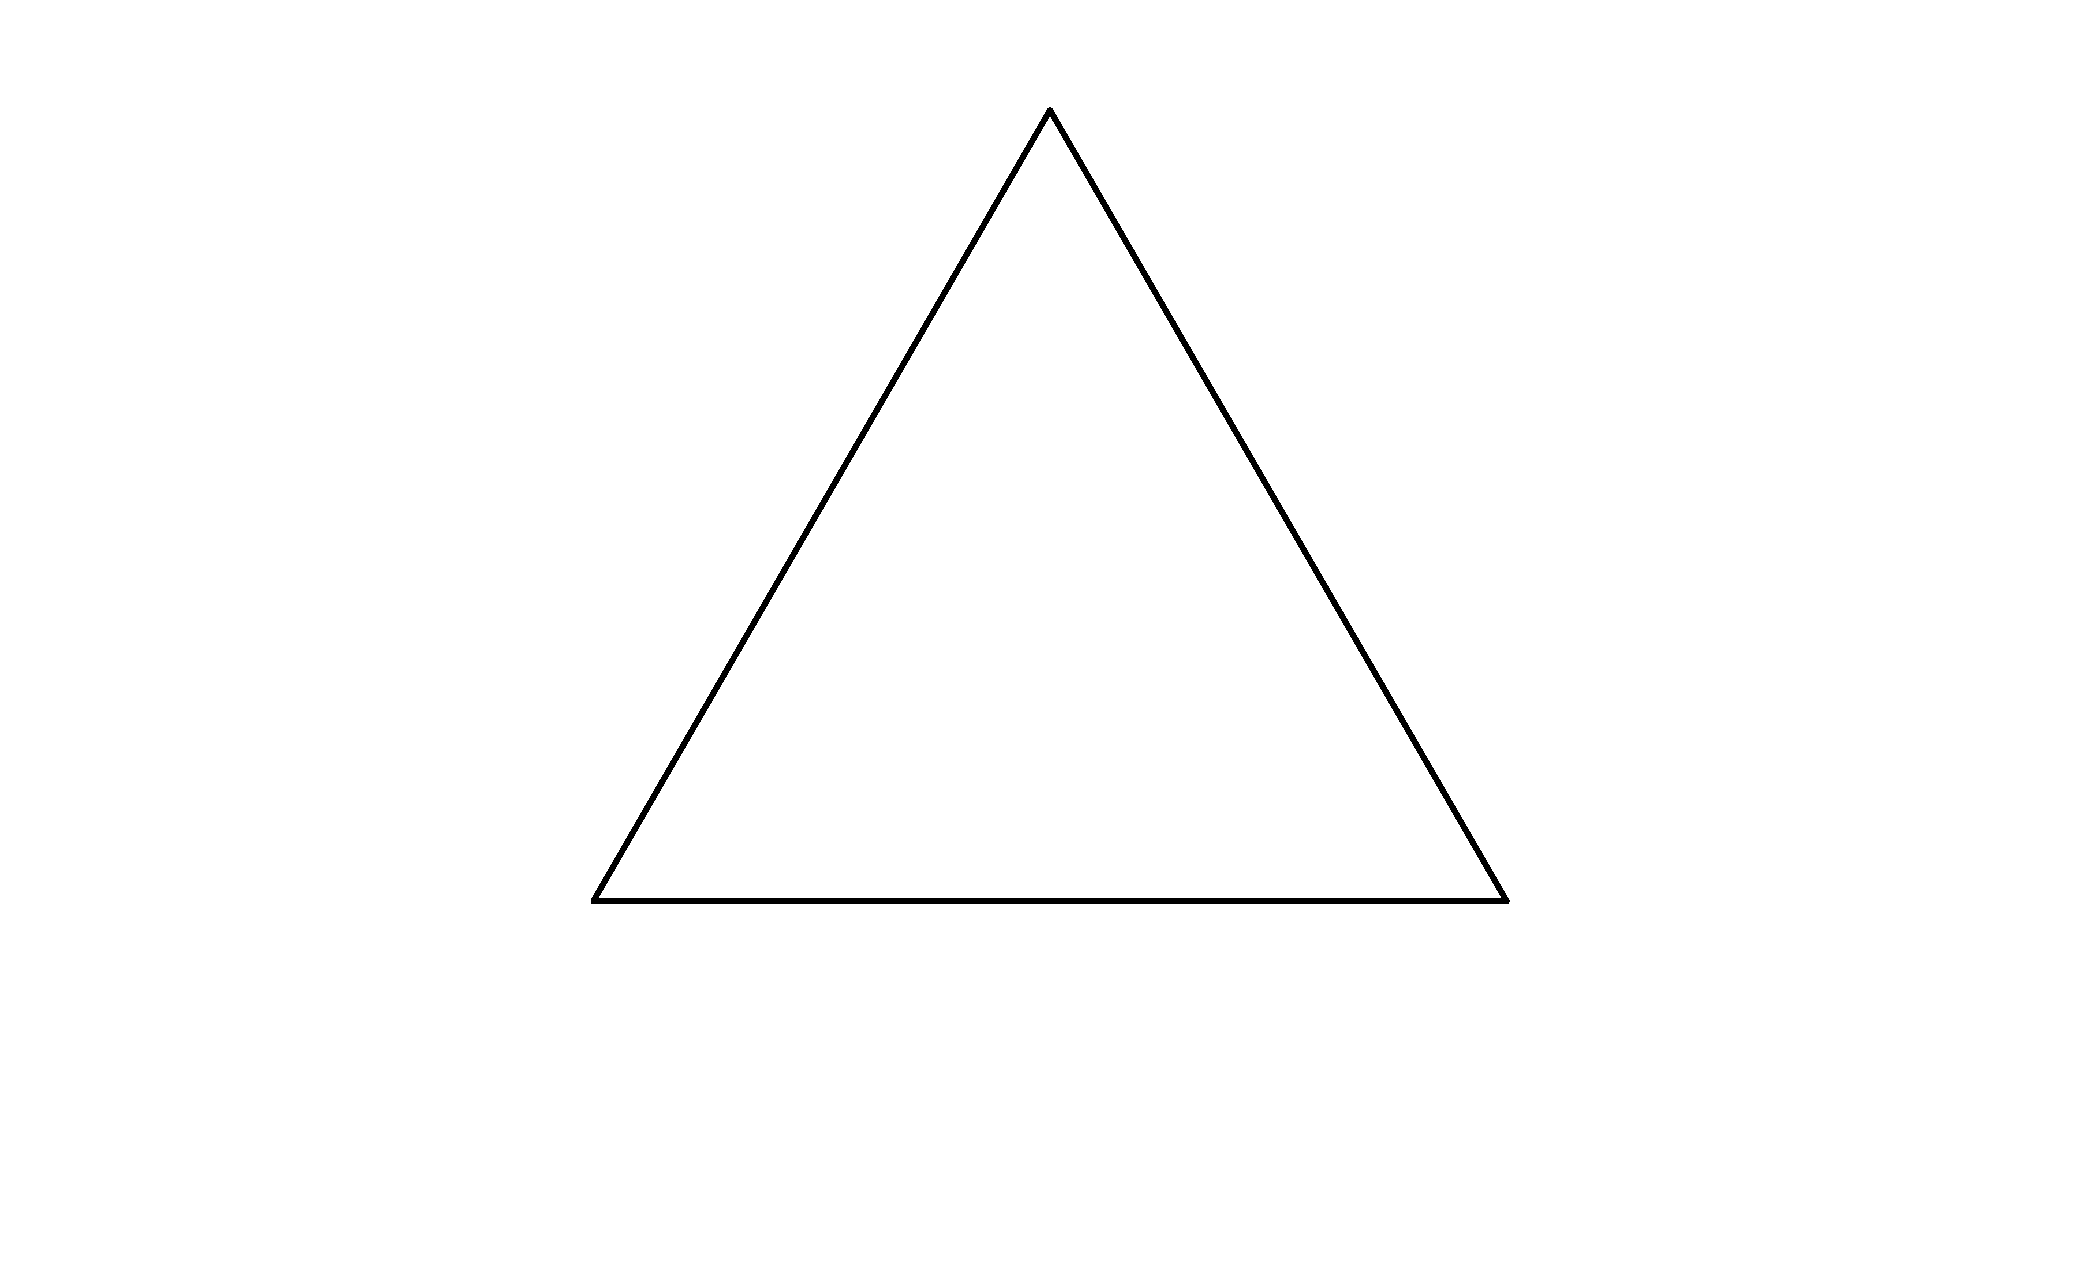
\includegraphics[width=0.2\linewidth]{img/triangle.pdf} & 
		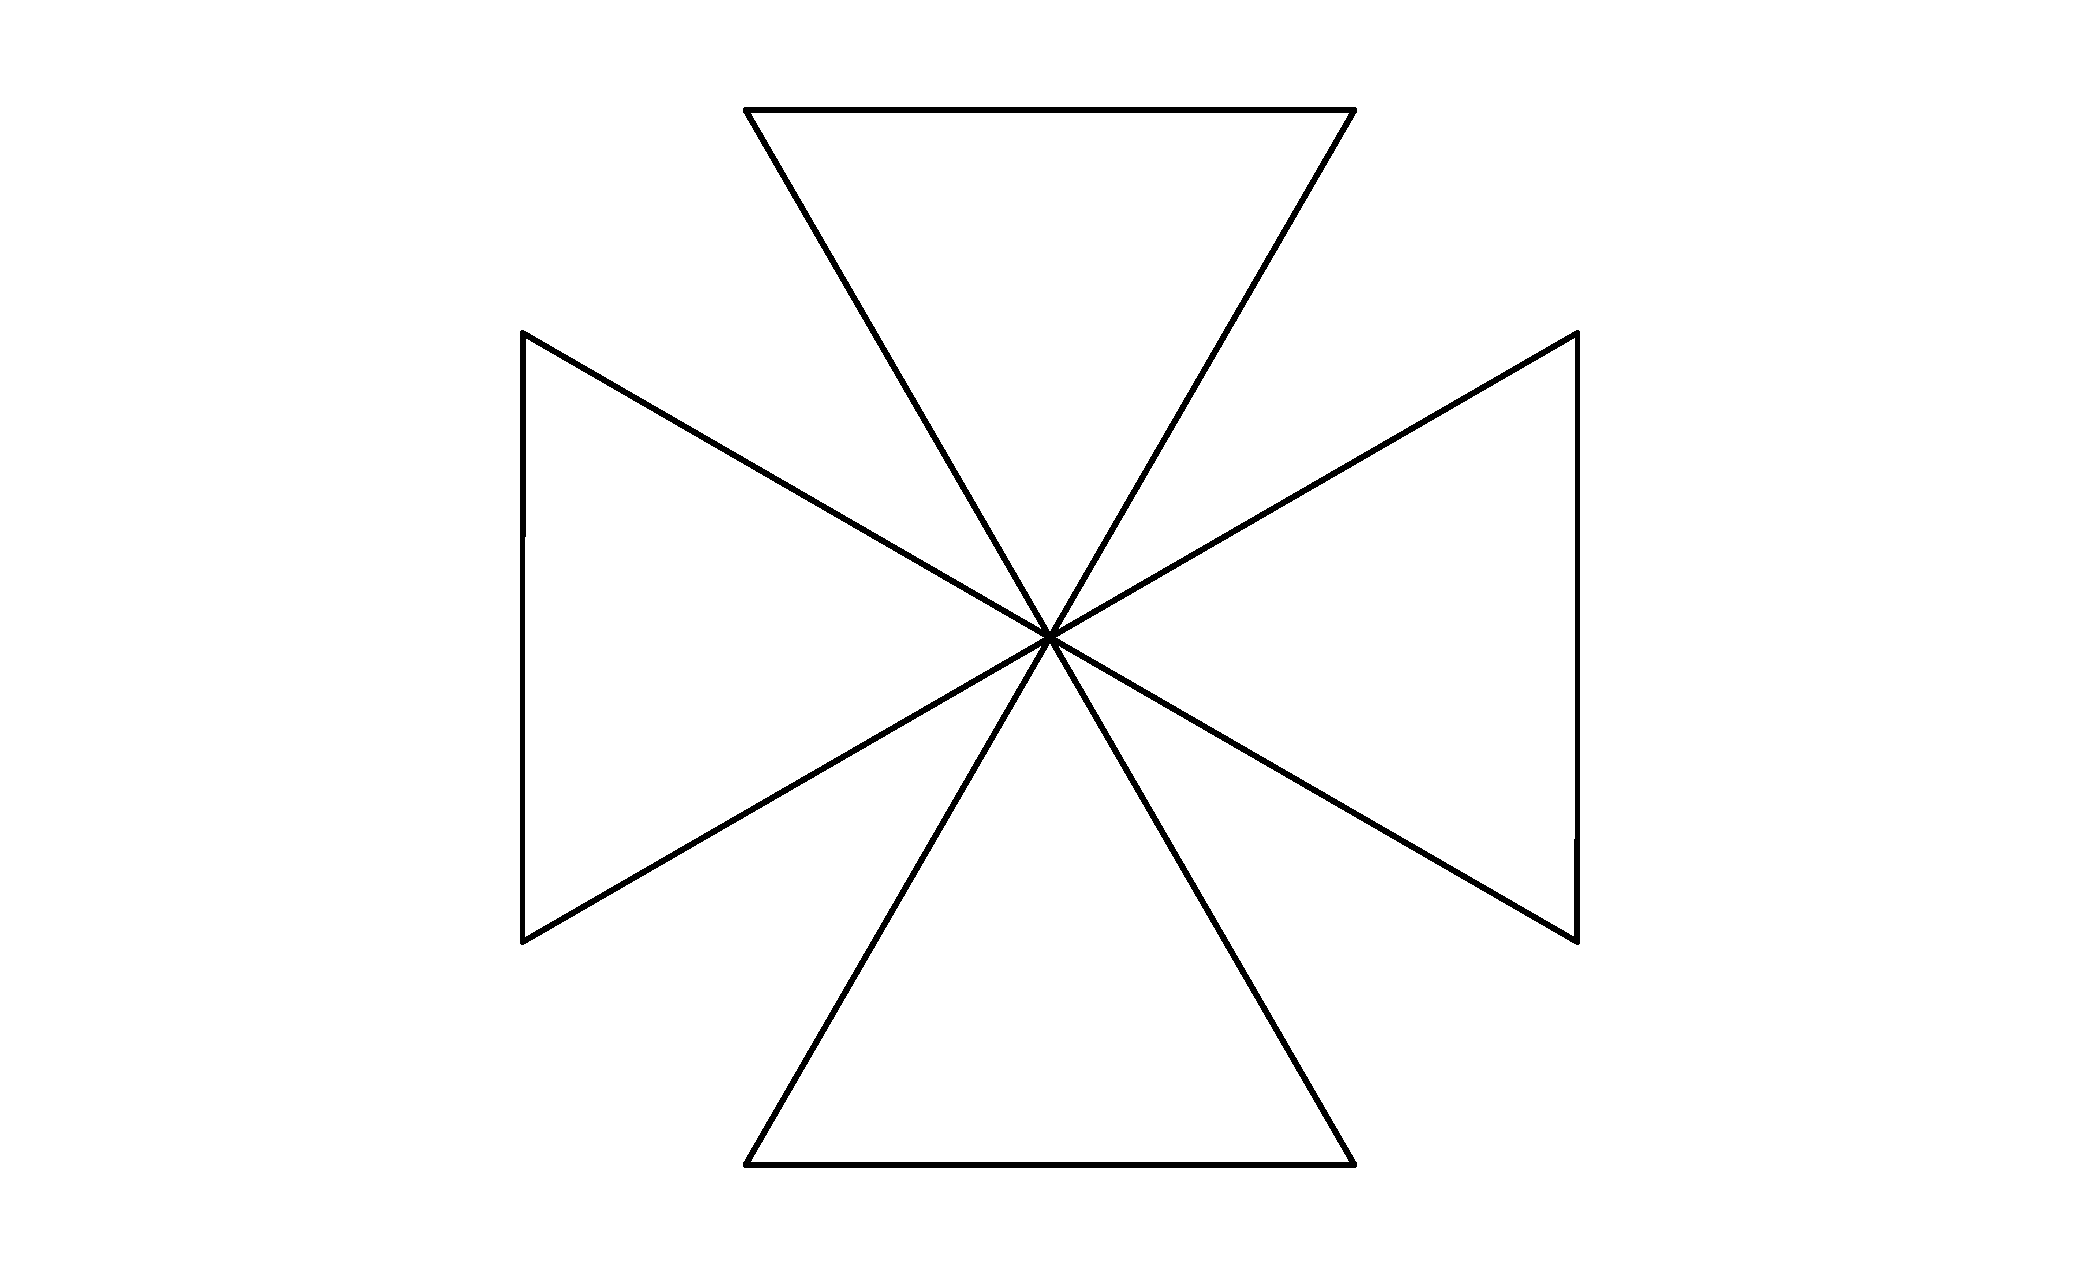
\includegraphics[width=0.2\linewidth]{img/malta.pdf} & 
		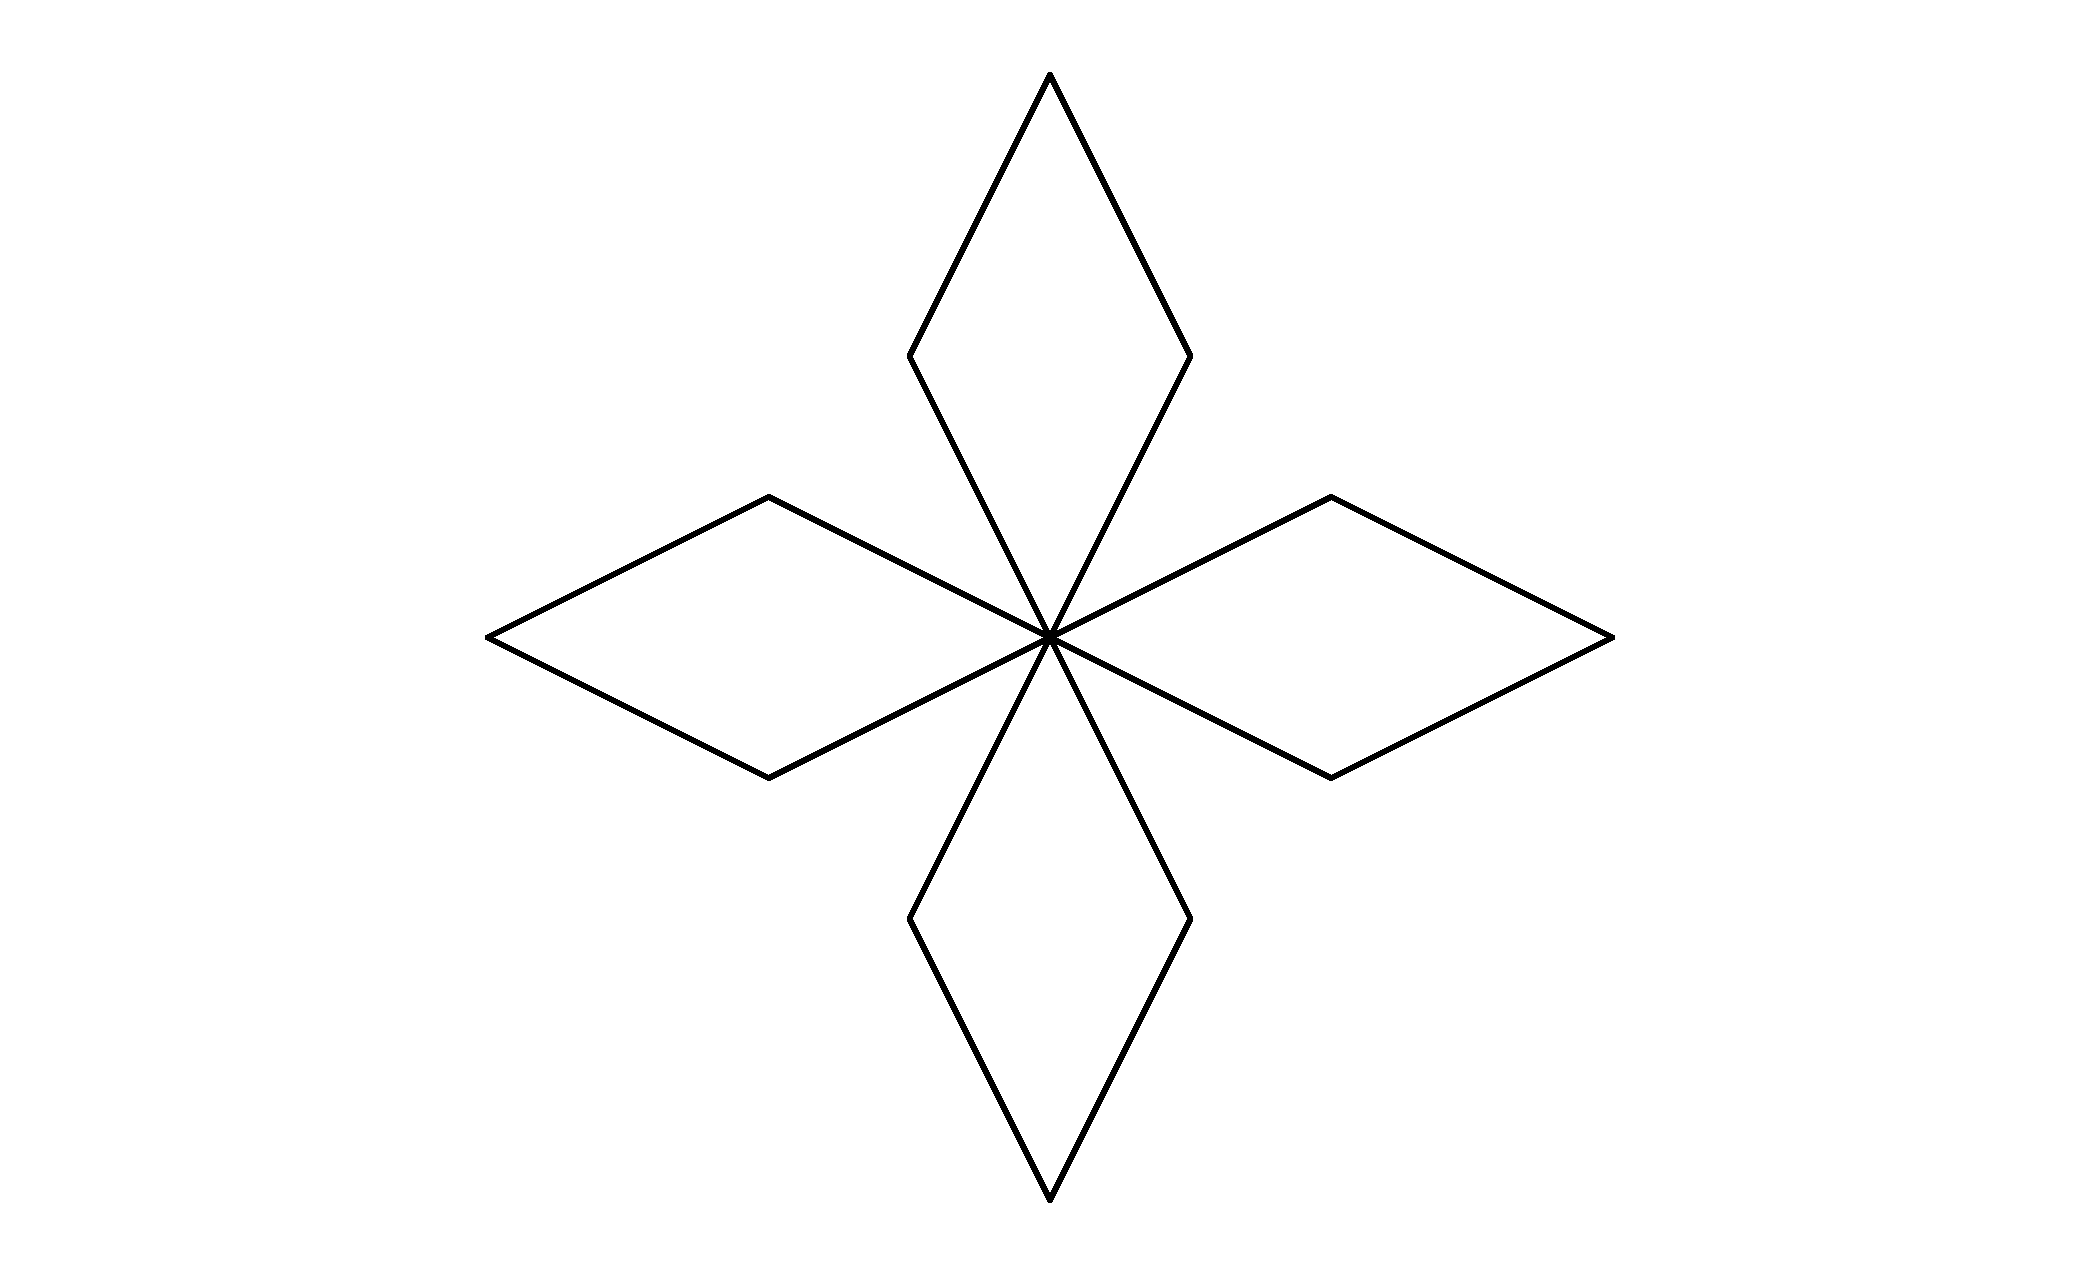
\includegraphics[width=0.2\linewidth]{img/maxi.pdf} \\
		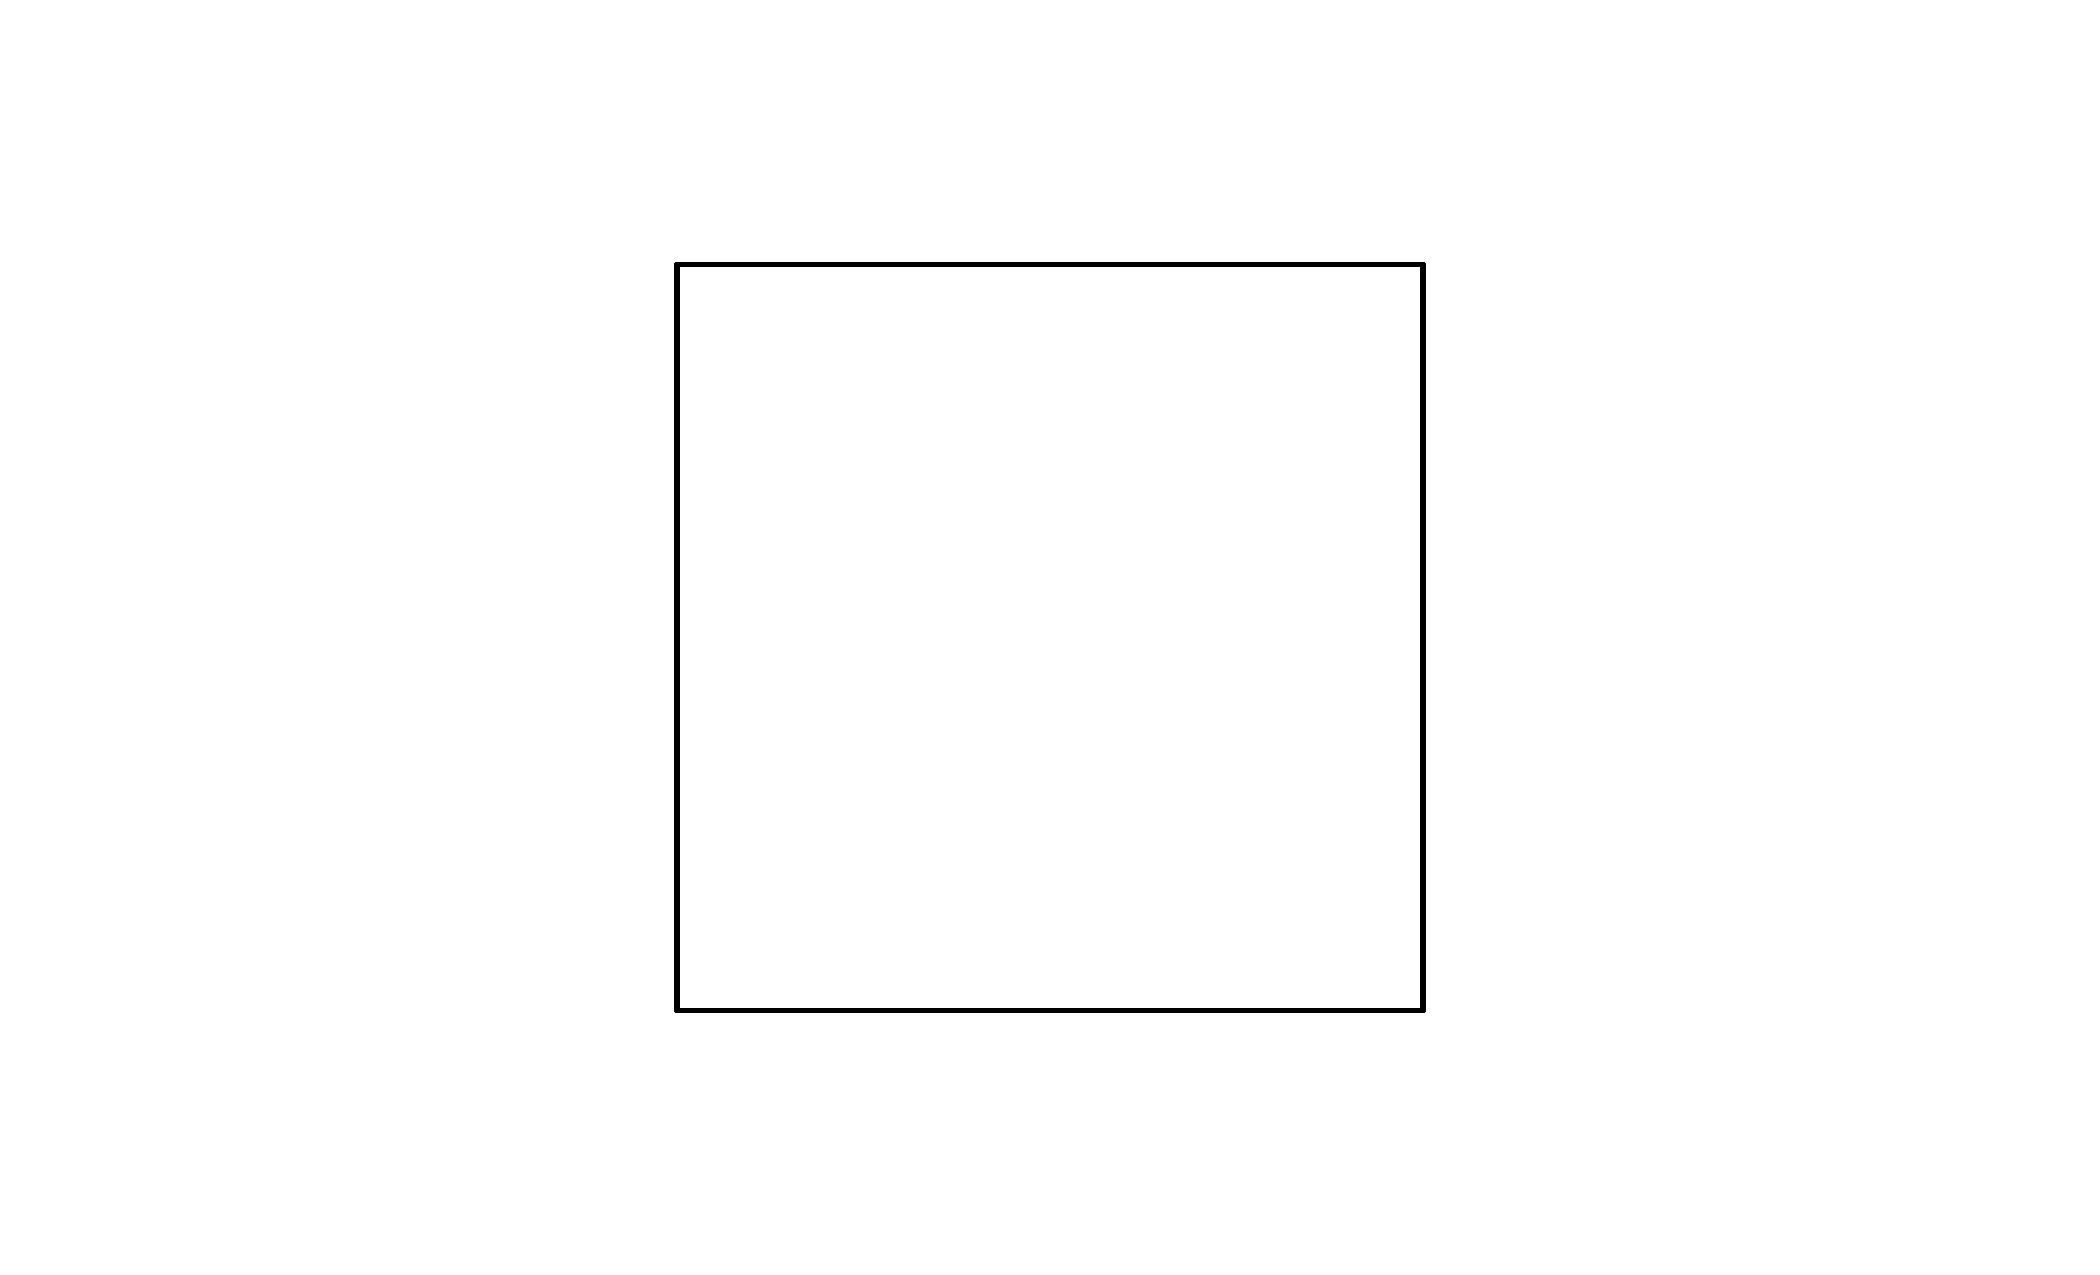
\includegraphics[width=0.2\linewidth]{img/square.pdf} & 
		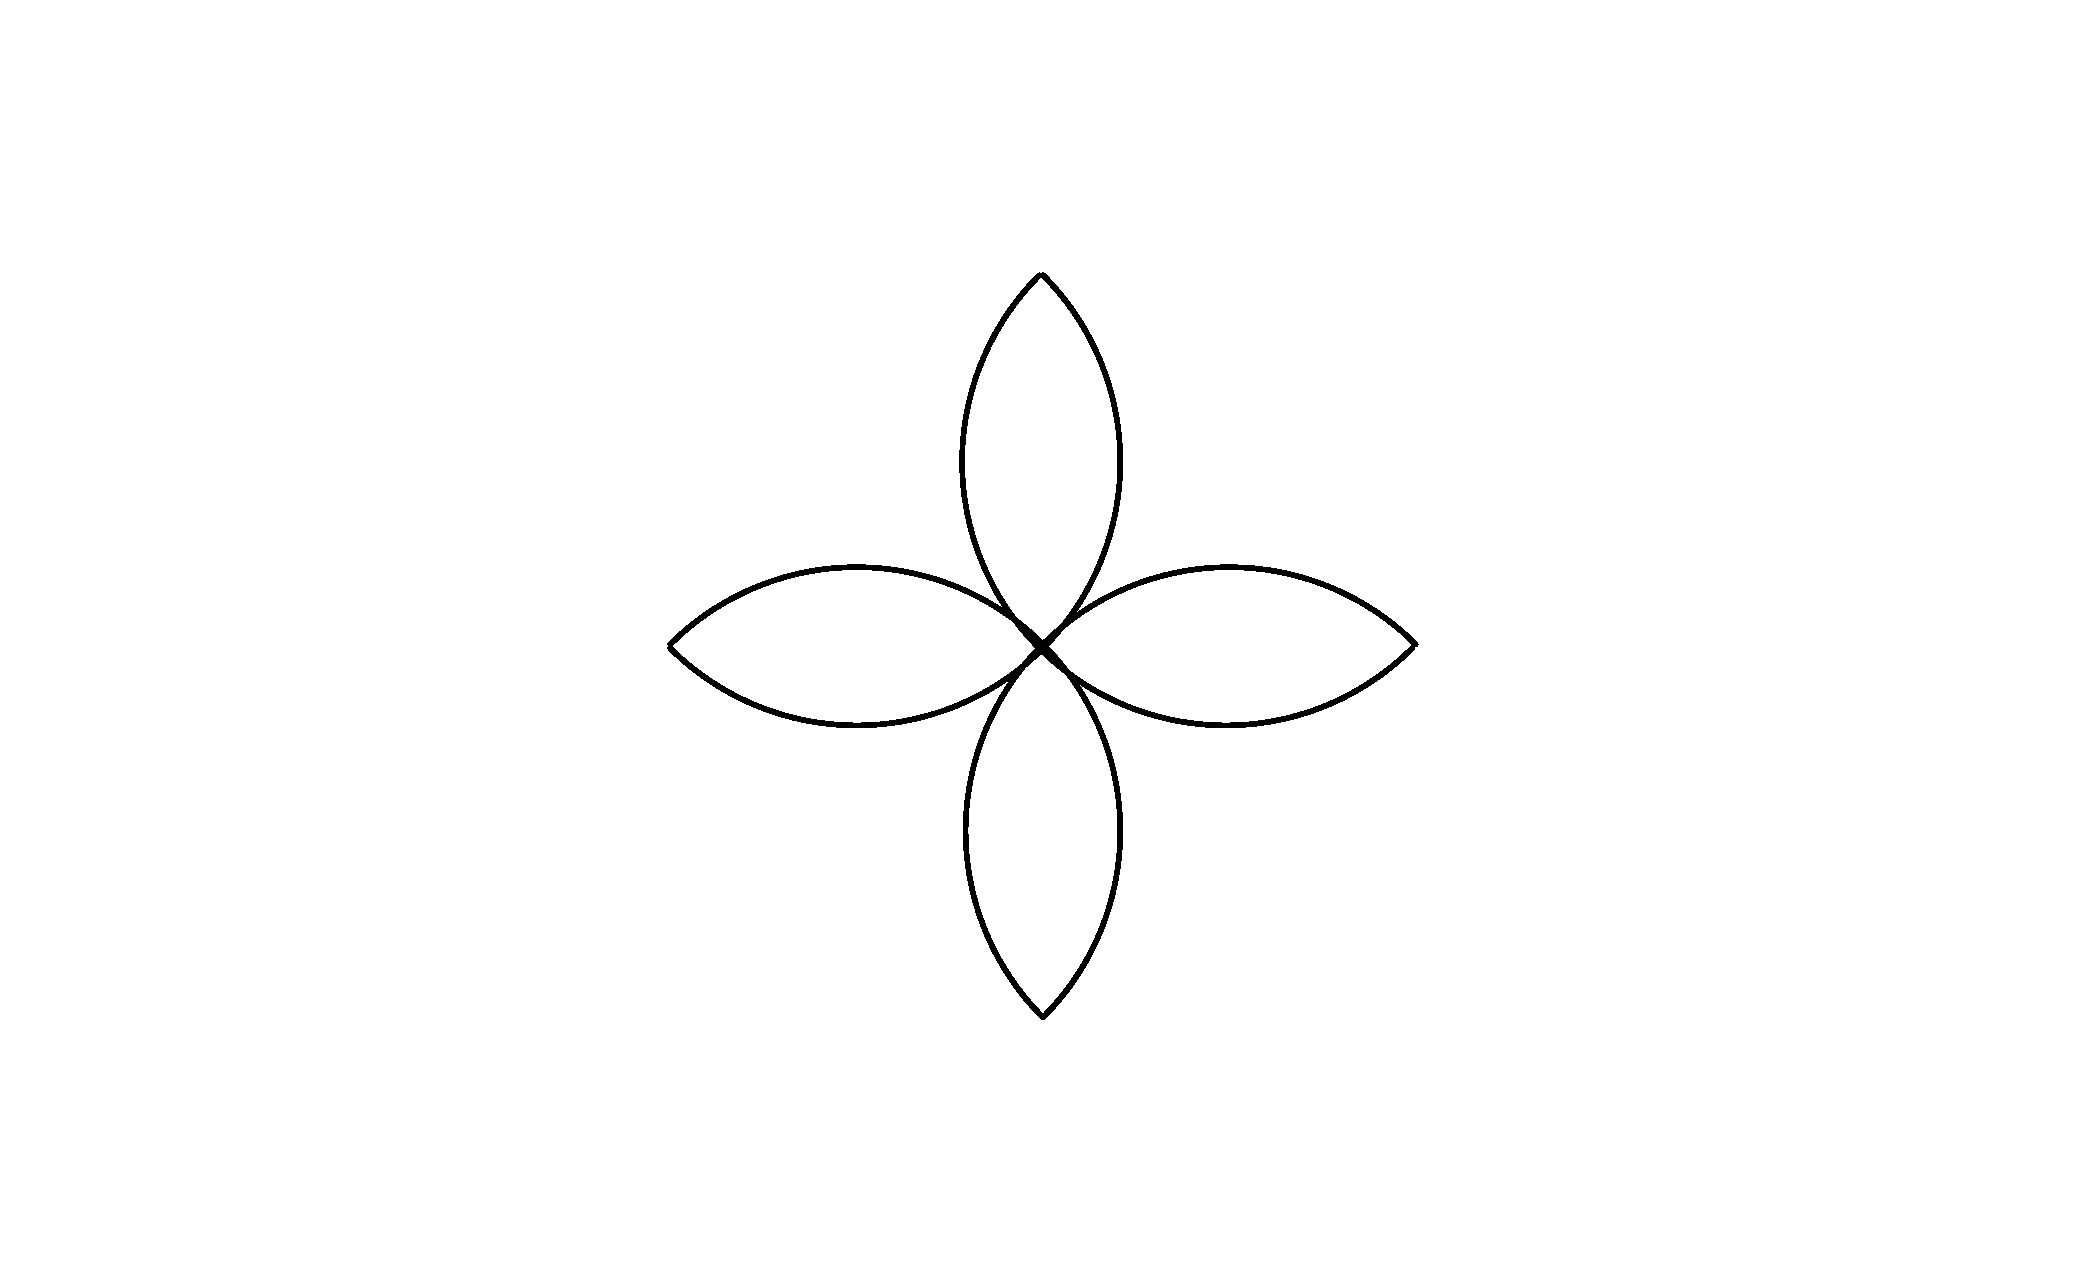
\includegraphics[width=0.2\linewidth]{img/lily.pdf} & 
		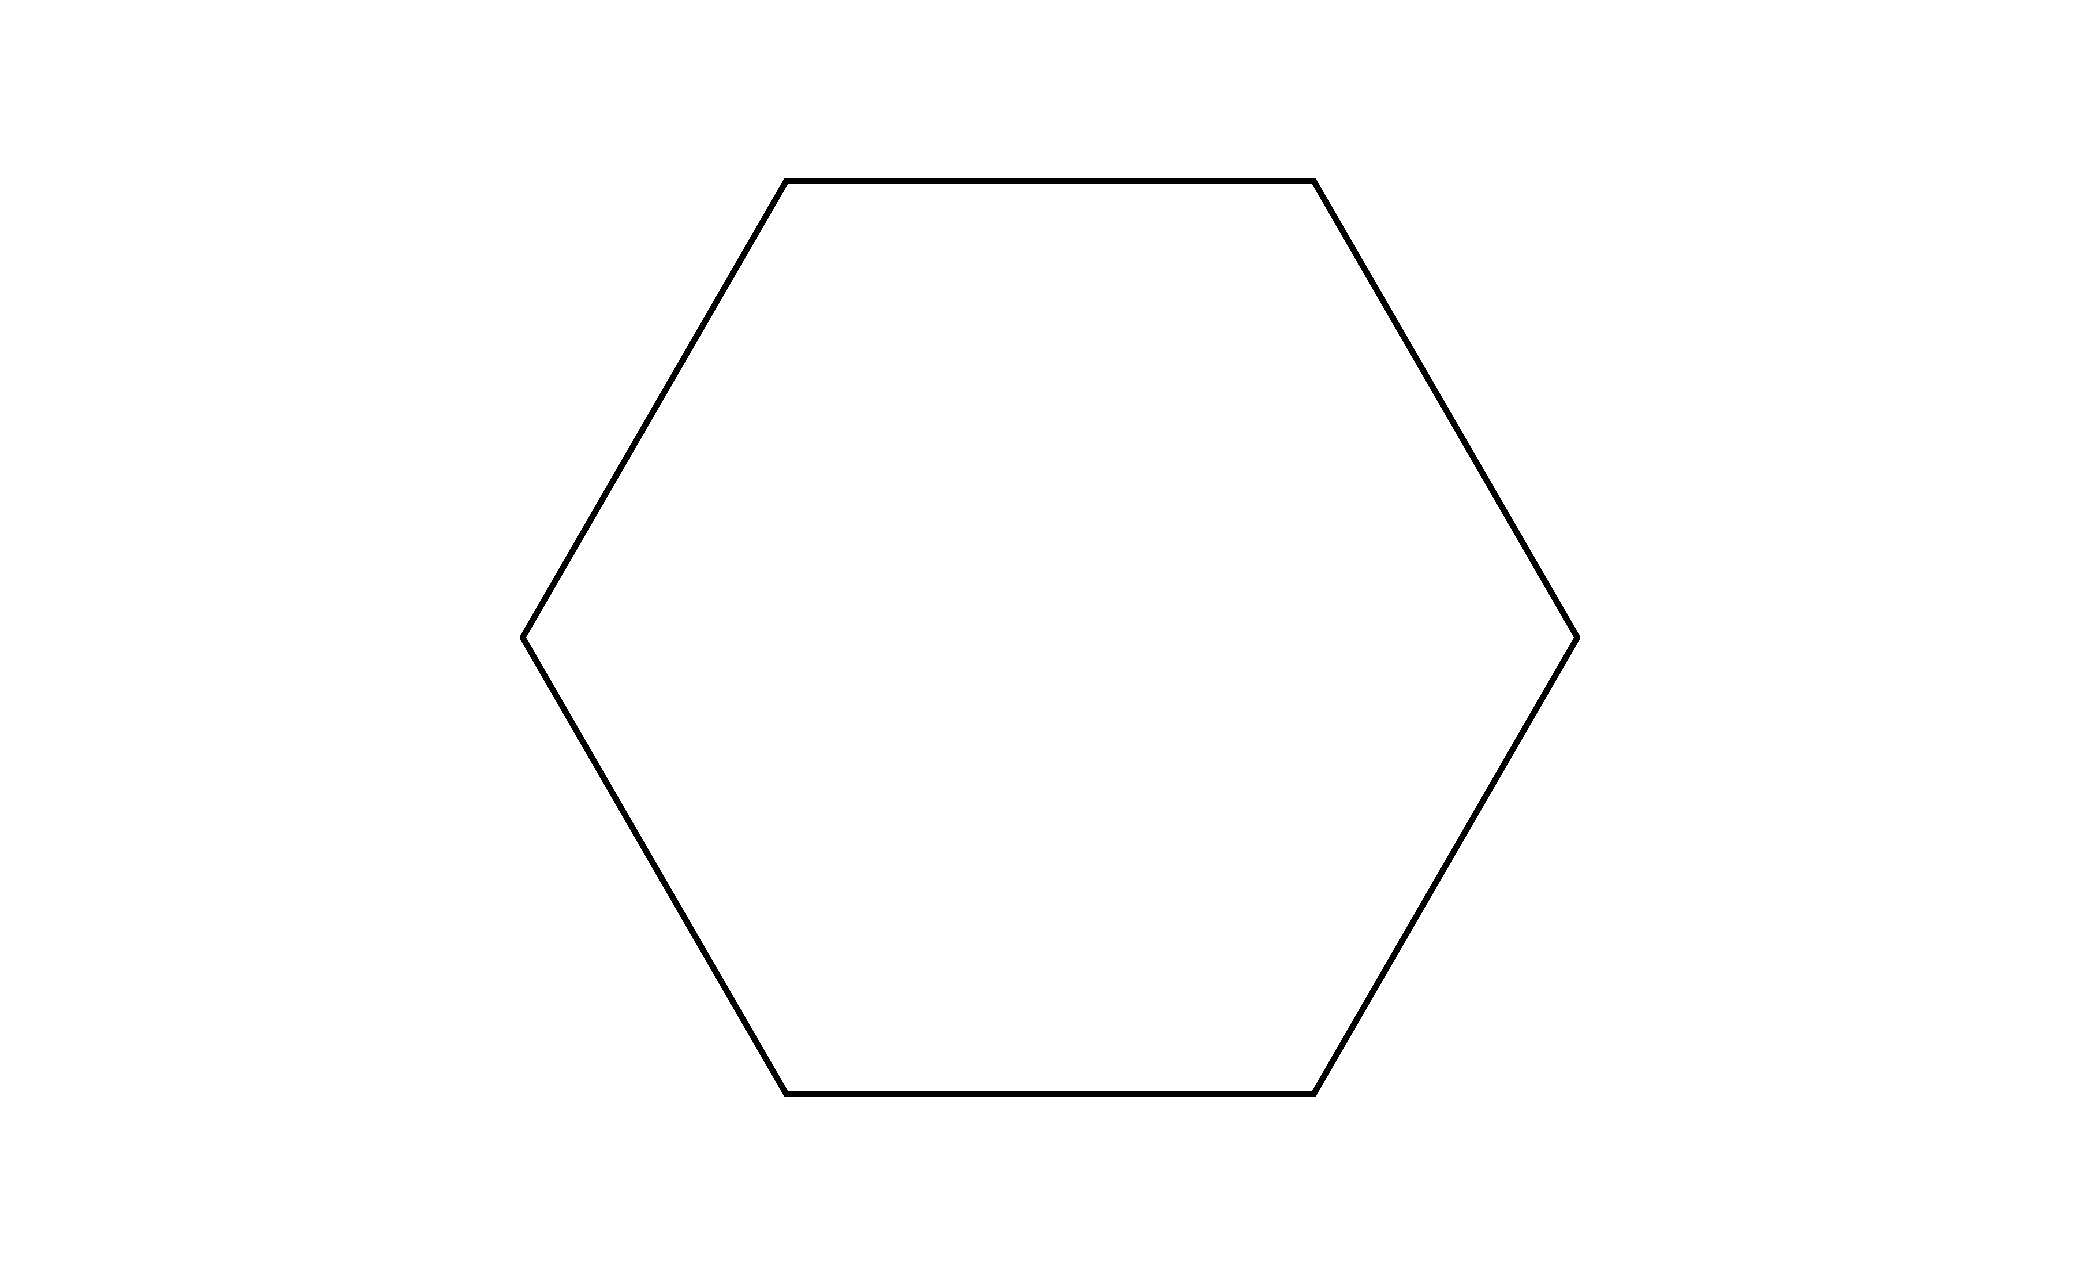
\includegraphics[width=0.2\linewidth]{img/hexagon.pdf} & 
		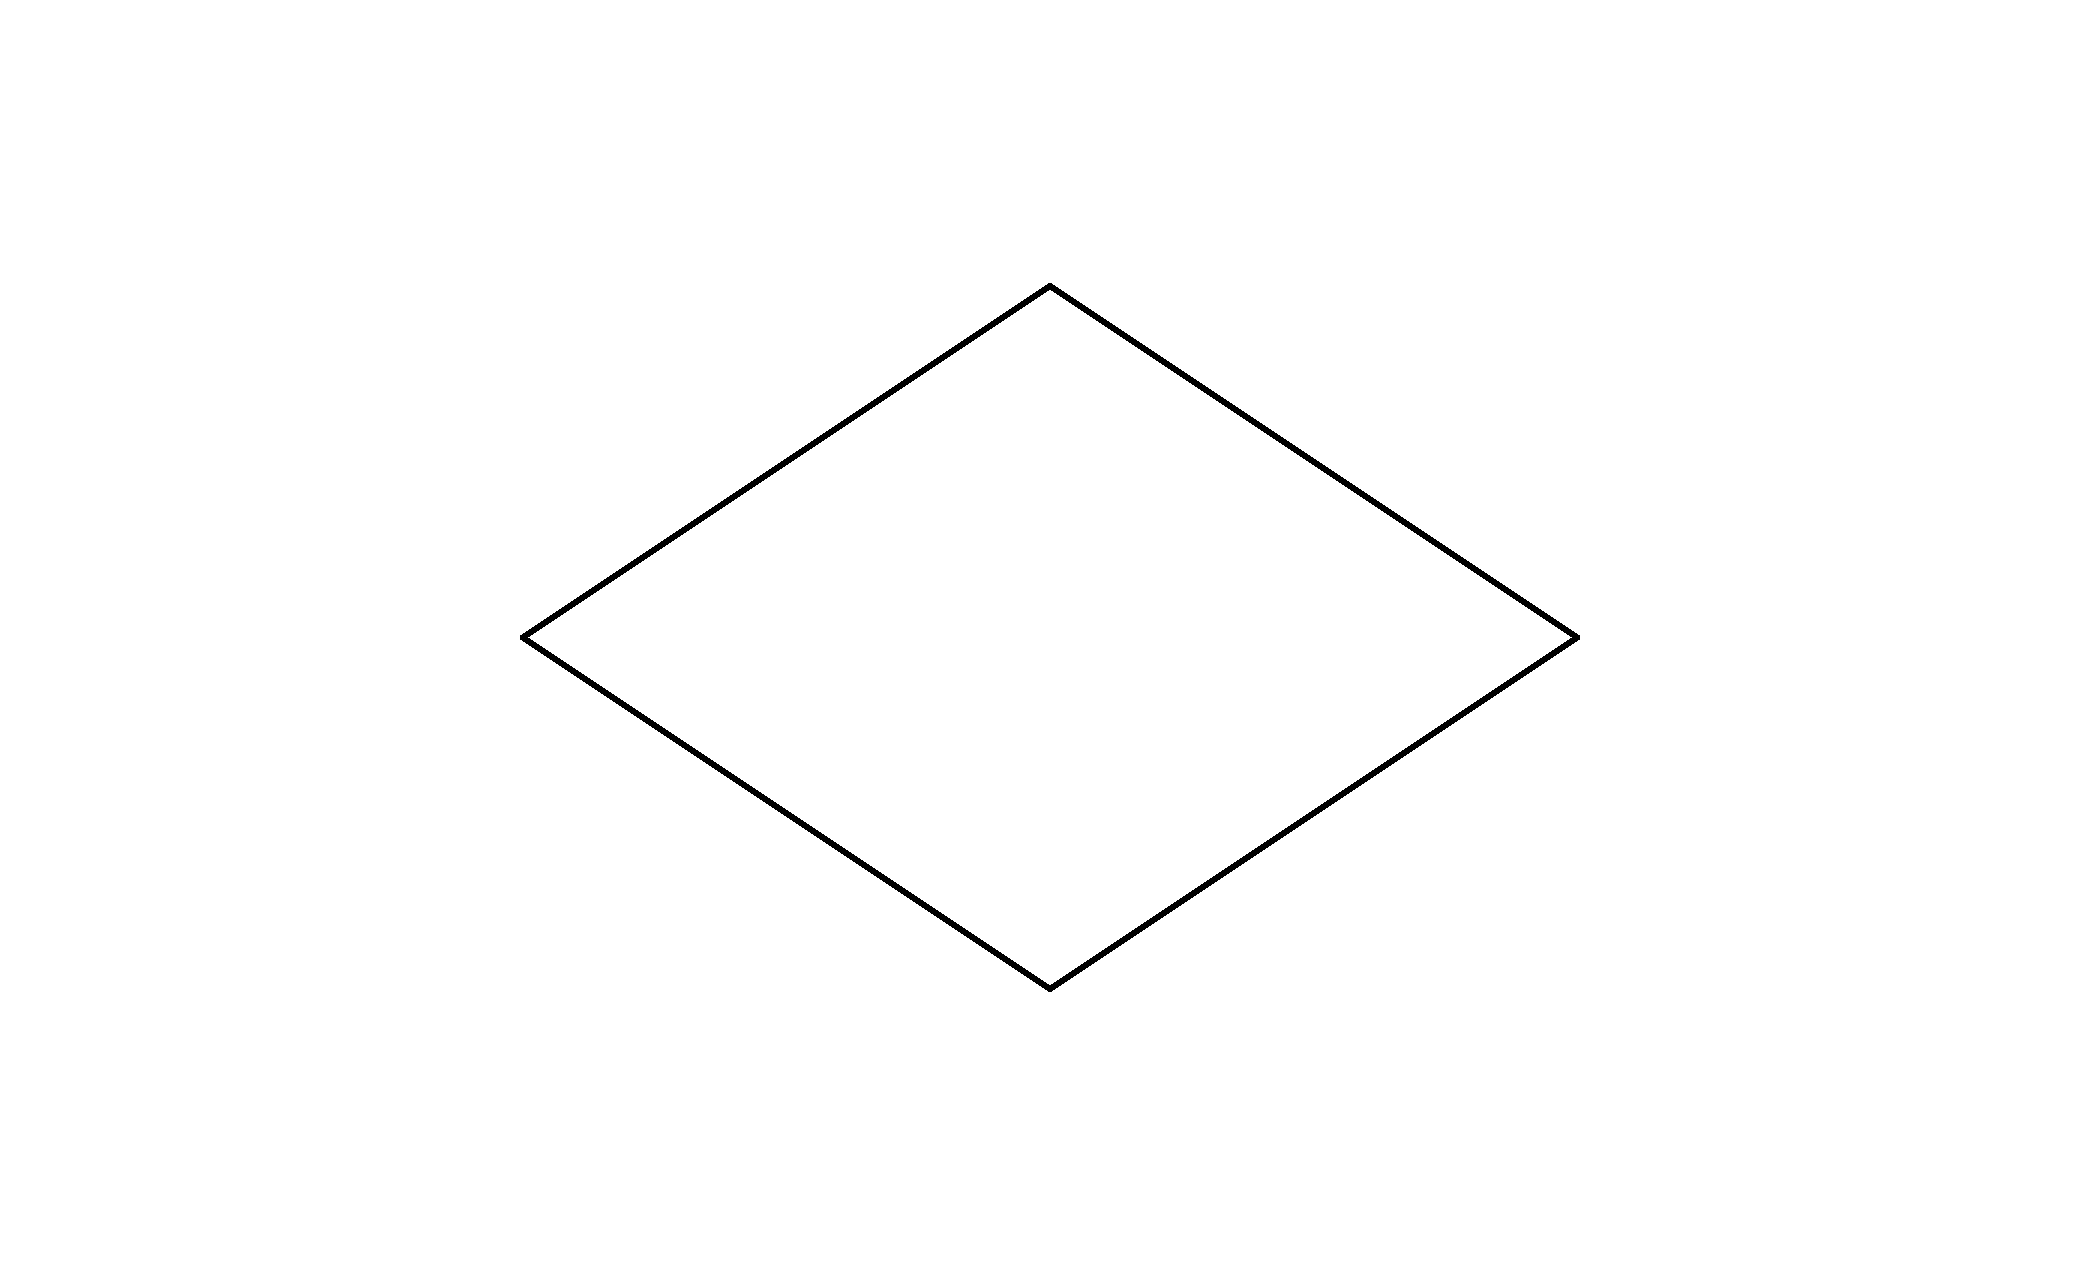
\includegraphics[width=0.2\linewidth]{img/luck.pdf} \\
		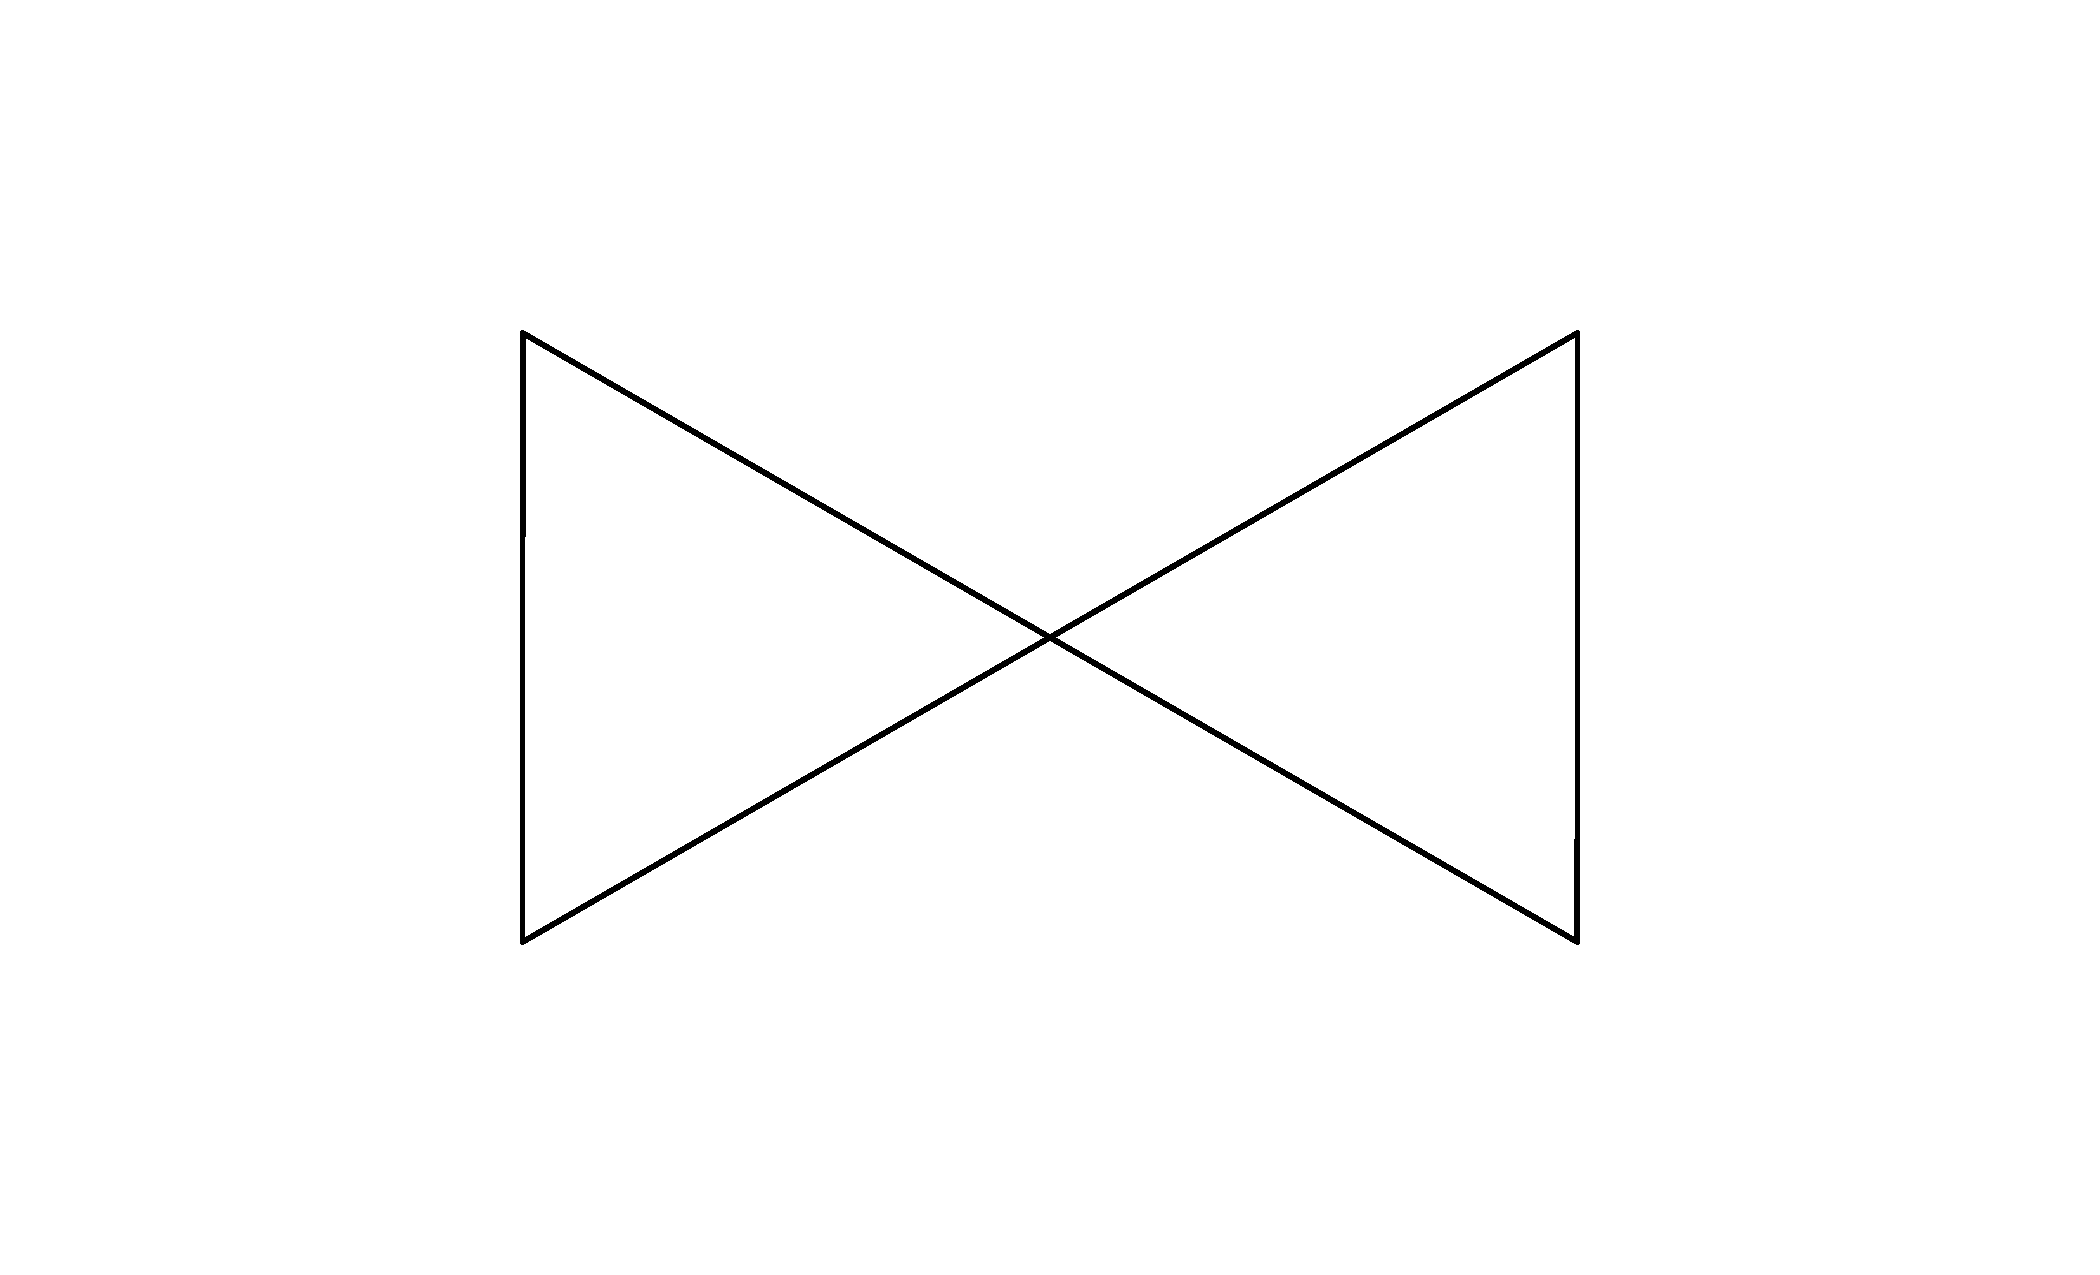
\includegraphics[width=0.2\linewidth]{img/bowtie.pdf} & 
		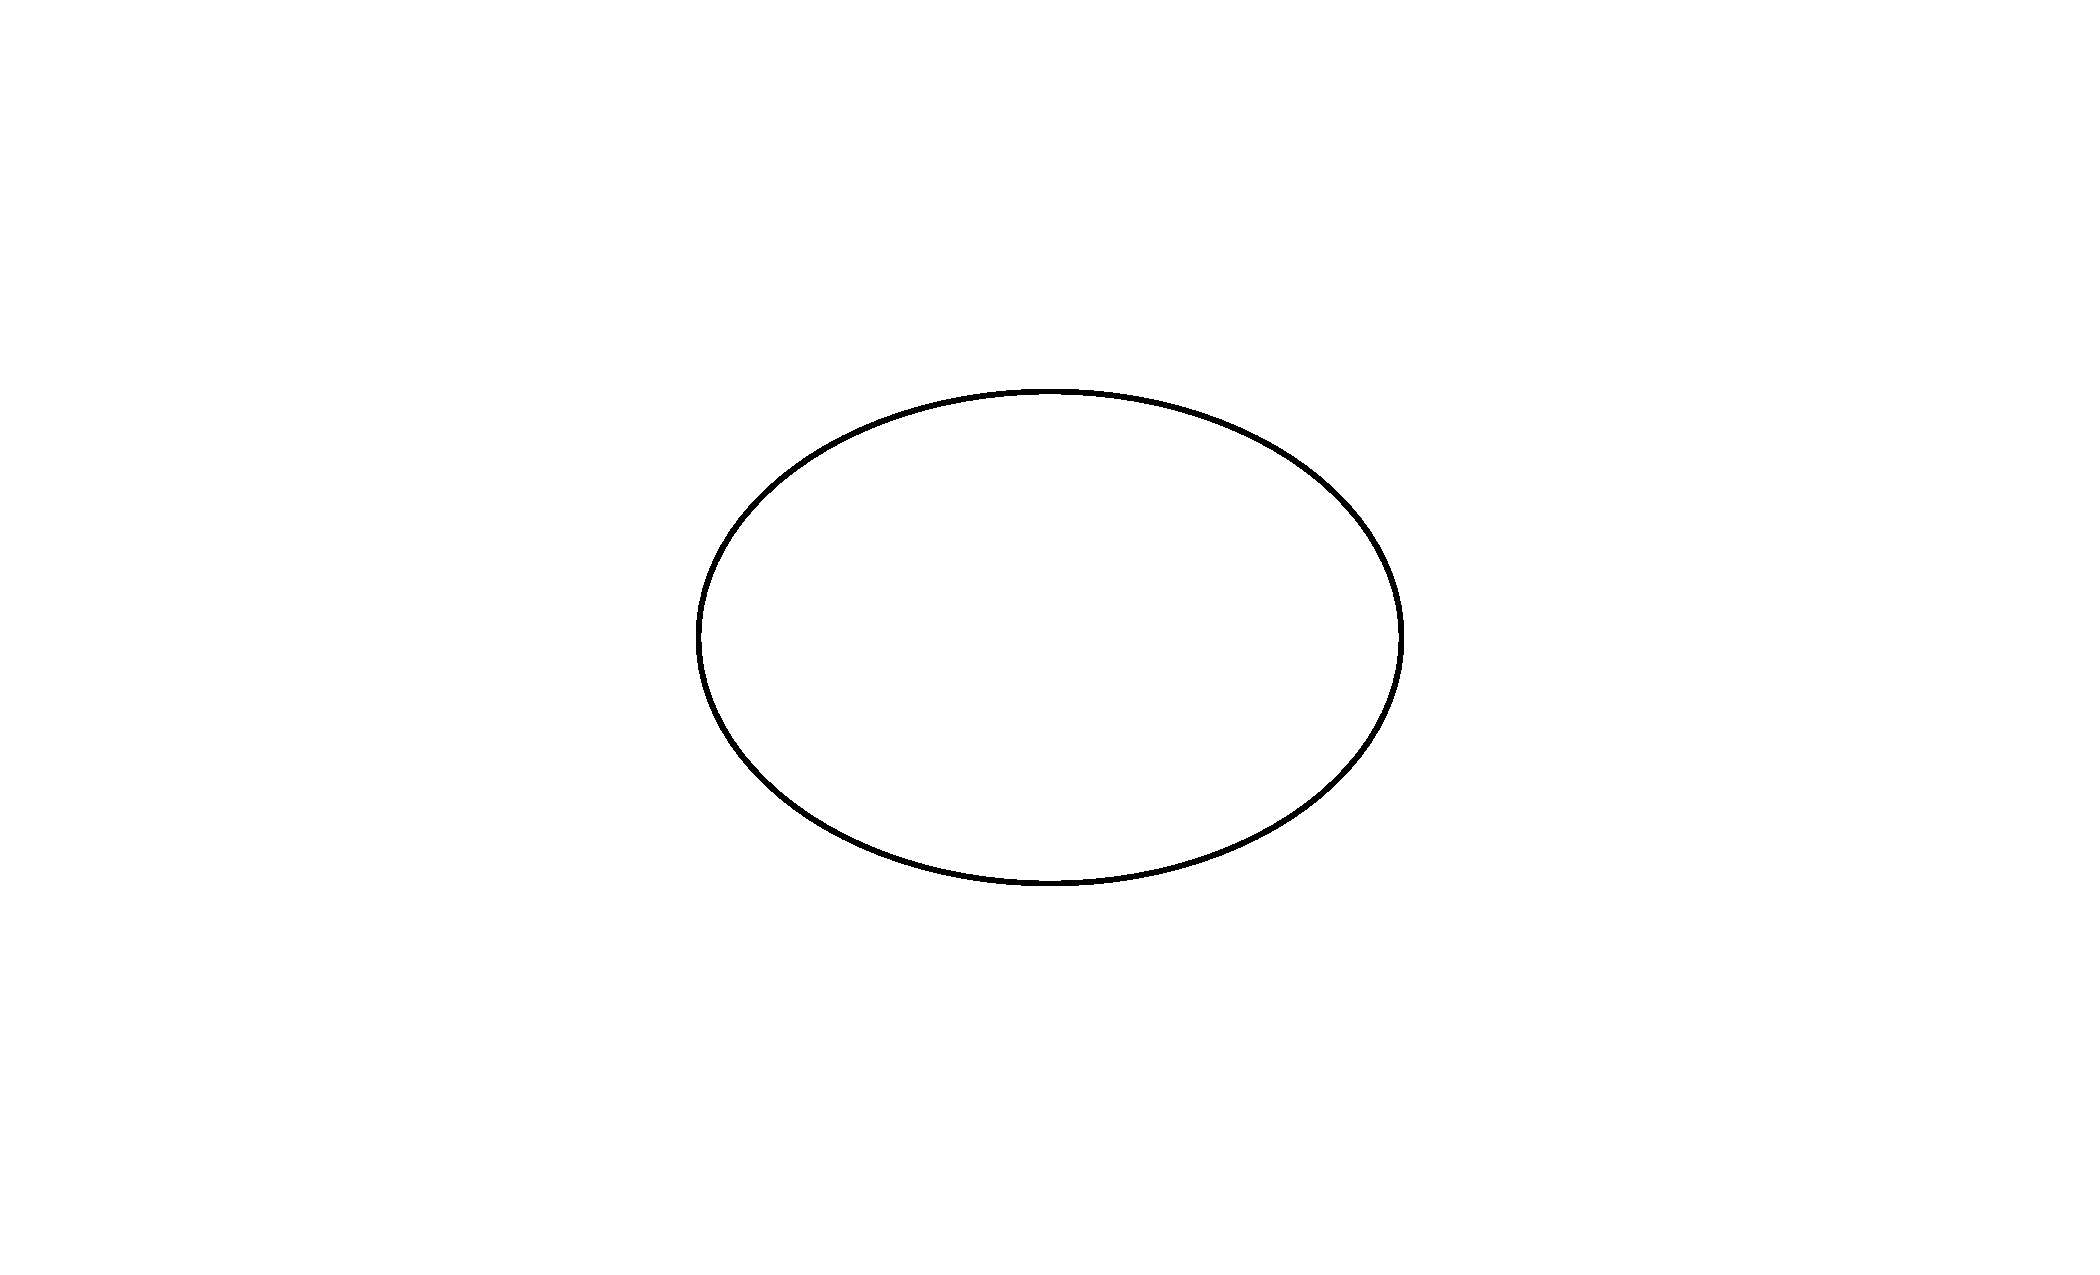
\includegraphics[width=0.2\linewidth]{img/ellipse.pdf} & 
		
\includegraphics[width=0.2\linewidth]{img/ninja.pdf} & 
		
\includegraphics[width=0.2\linewidth]{img/biscuit.pdf} \\
	\end{tabular}
	
	\vspace{5mm}
	\centering
	\Large
	$\ldots$
	
\end{frame}


\begin{frame}{Visuospatial rules}
	\begin{columns}[T]
		\begin{column}{.50\linewidth}
			\centering
			Rotate 
			
			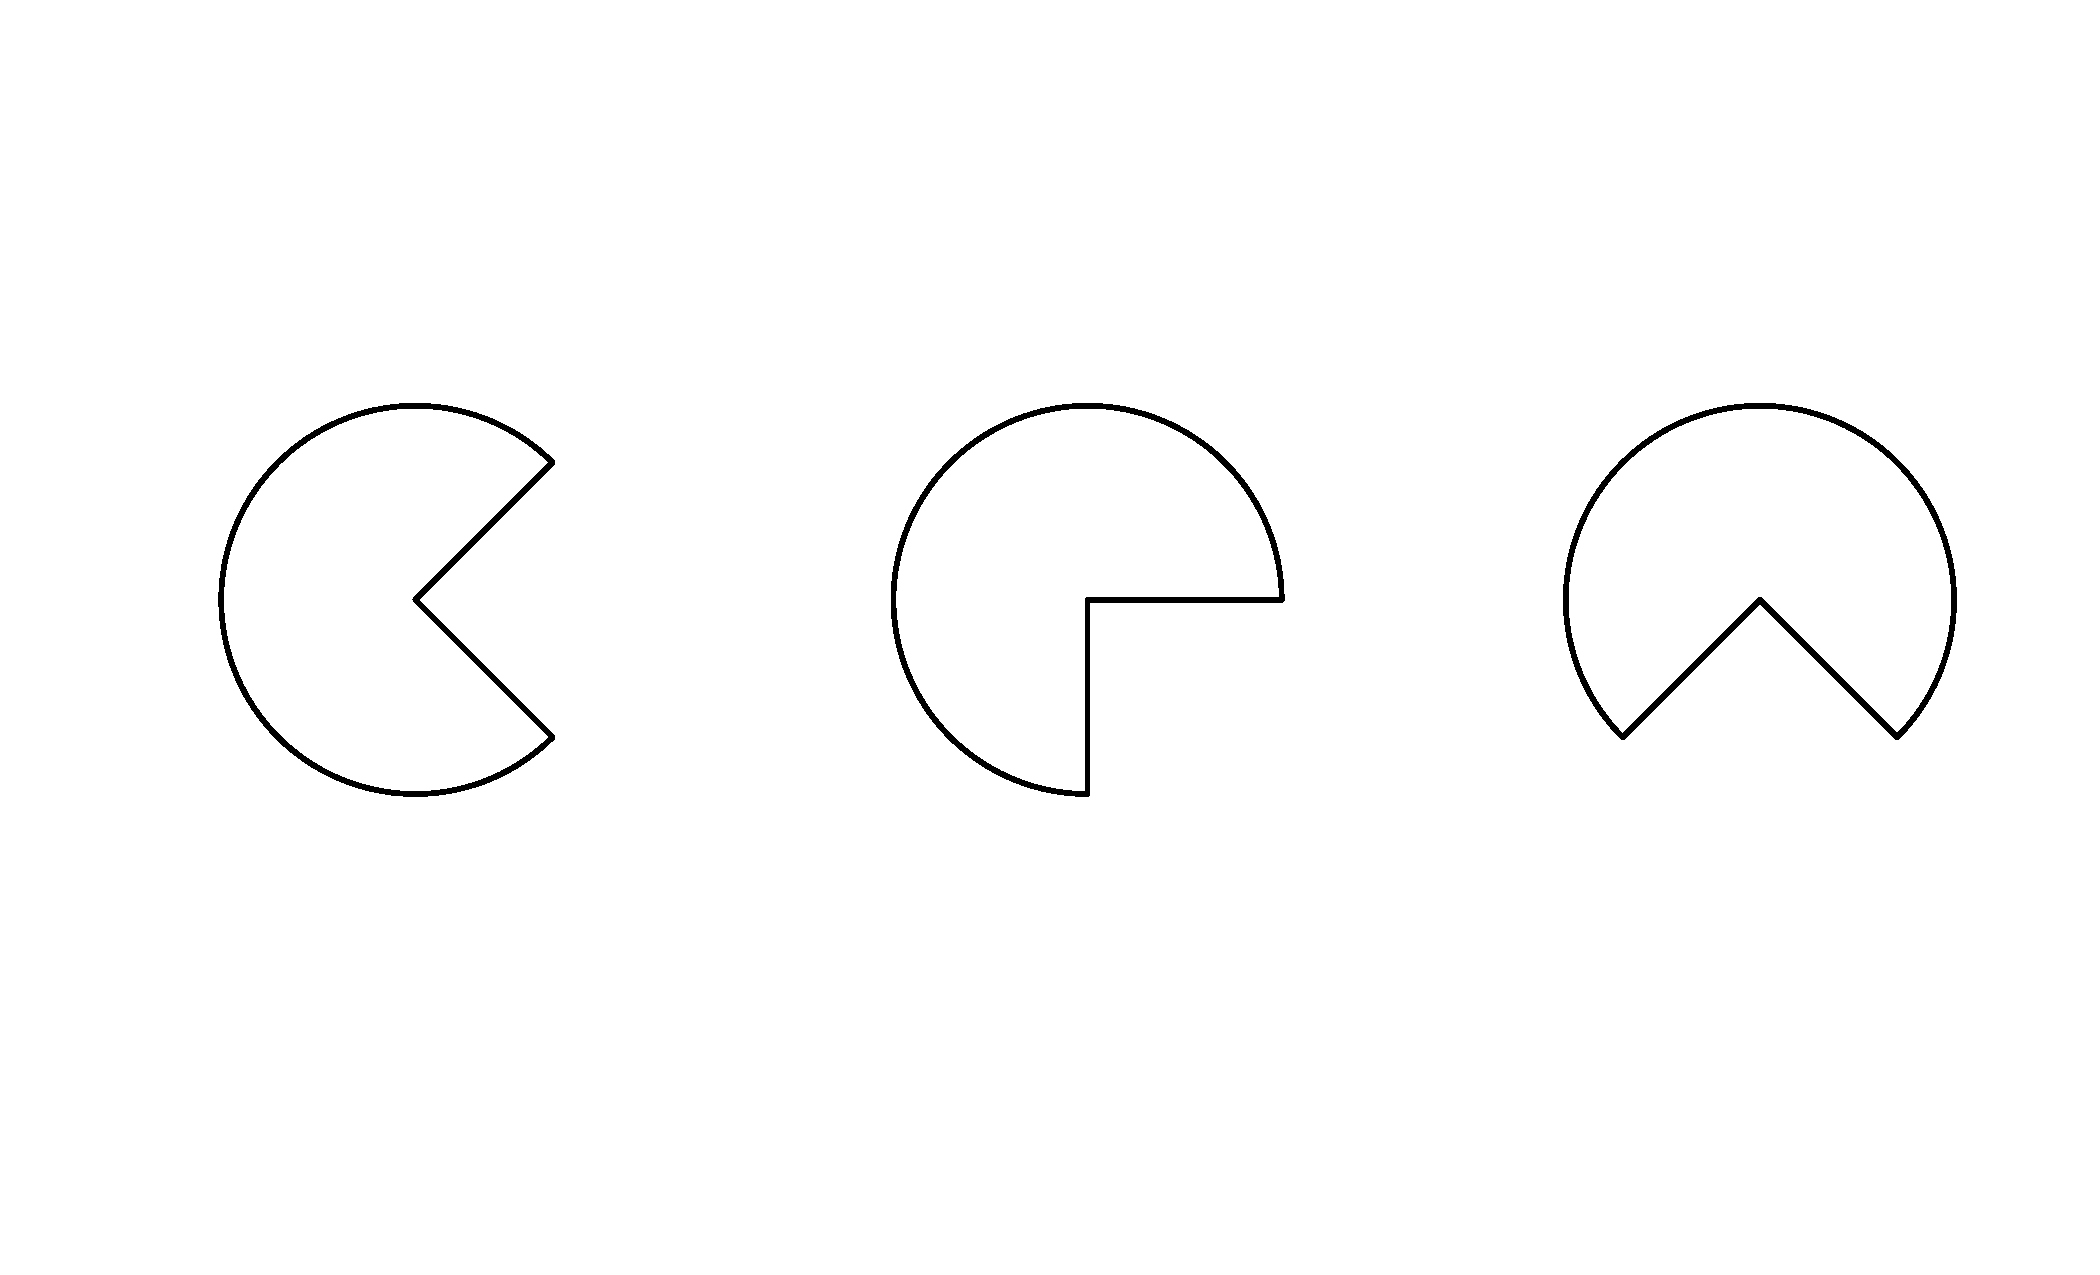
\includegraphics[width=.7\linewidth]{img/rotate.pdf}
			
			Shade
			
			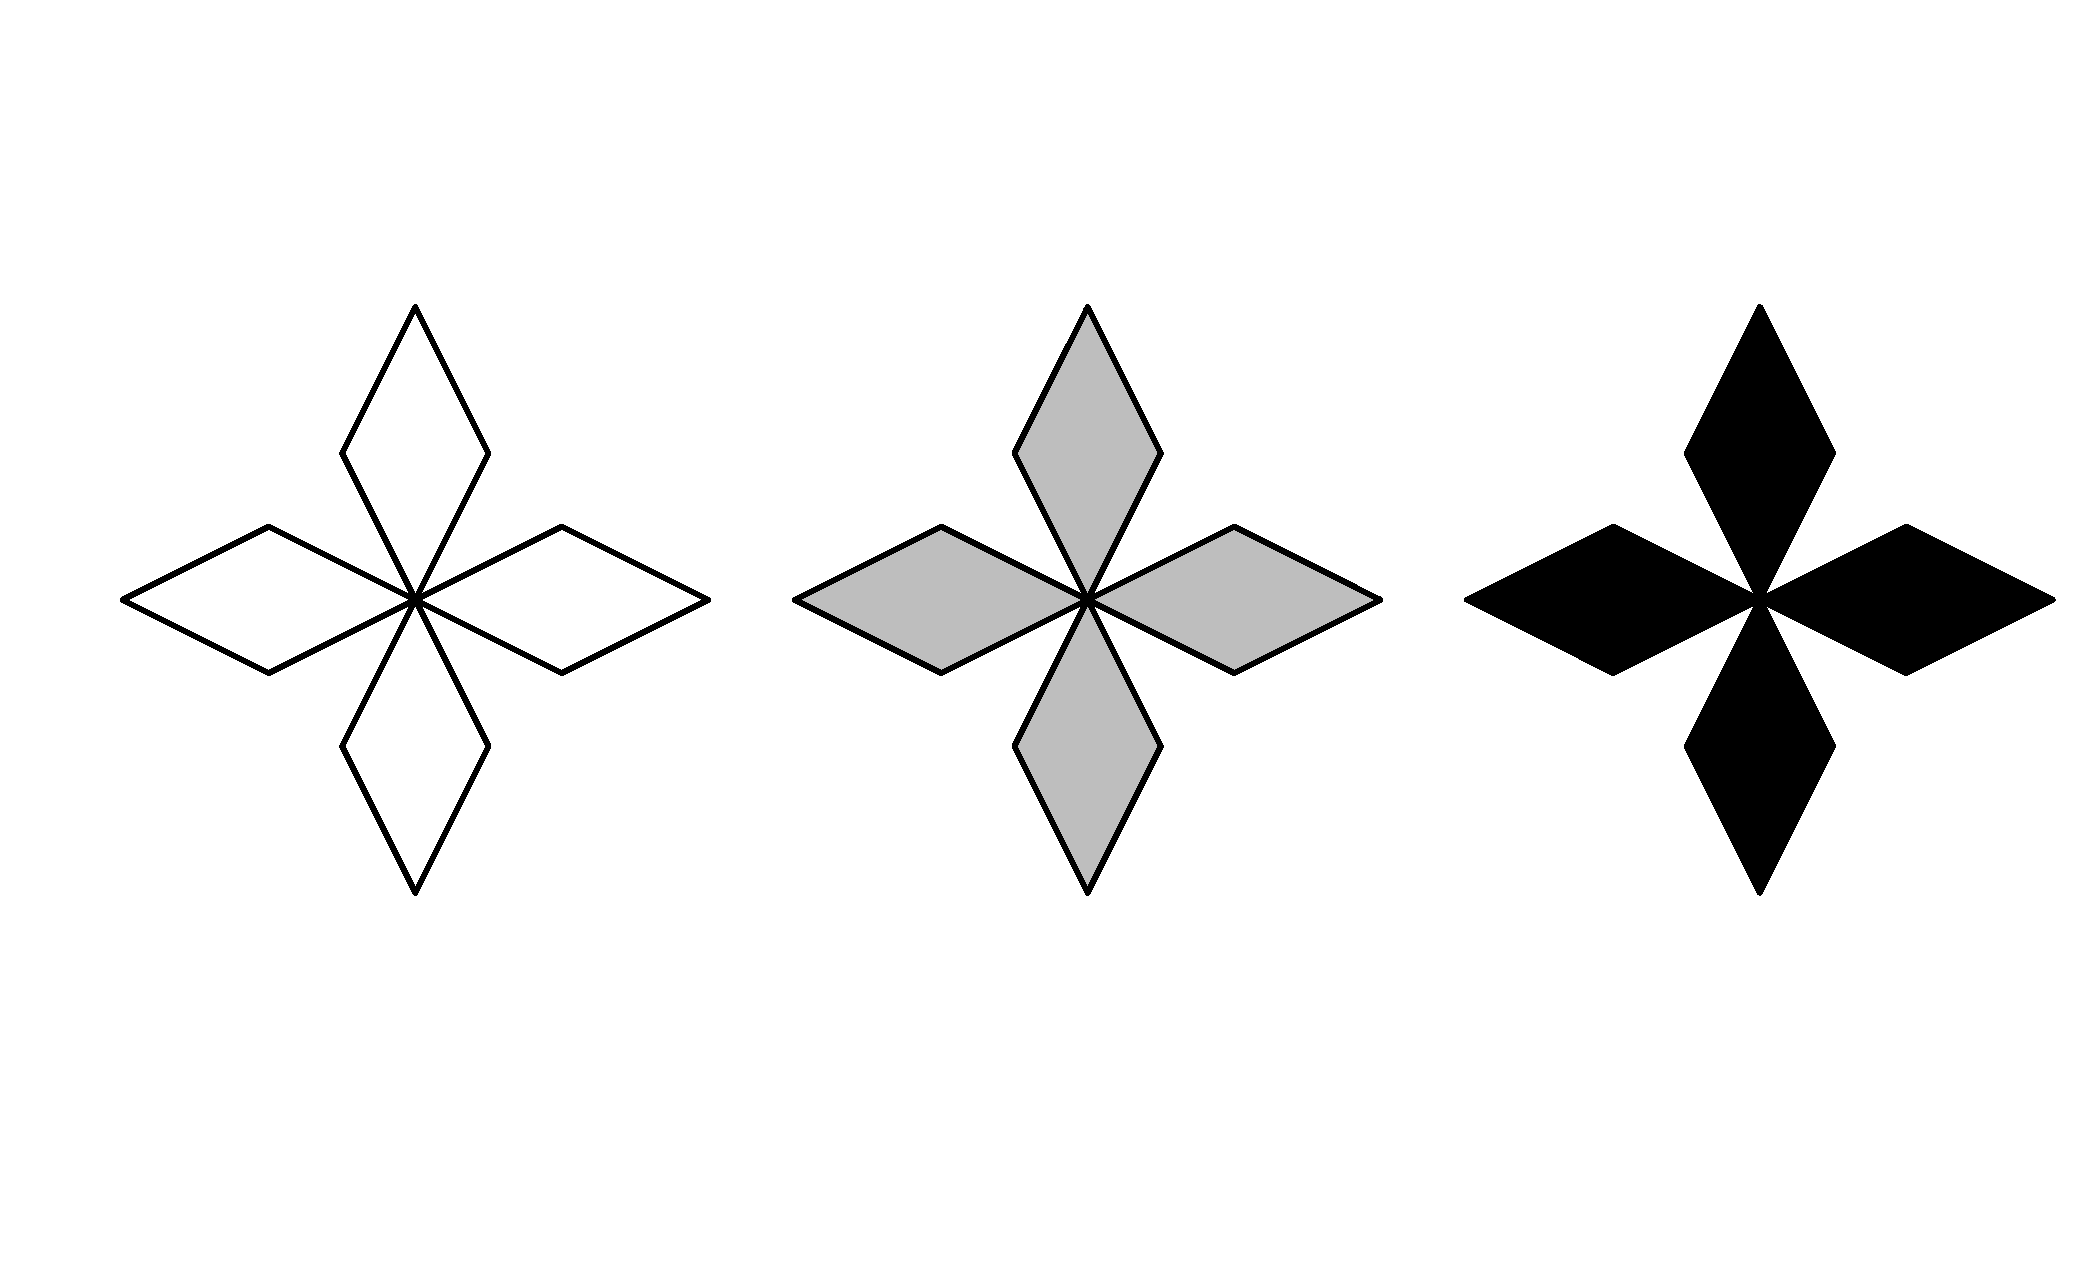
\includegraphics[width=.7\linewidth]{img/shade.pdf}
		\end{column}
		
		\begin{column}{.50\linewidth}
			\centering
			Shape 
			
			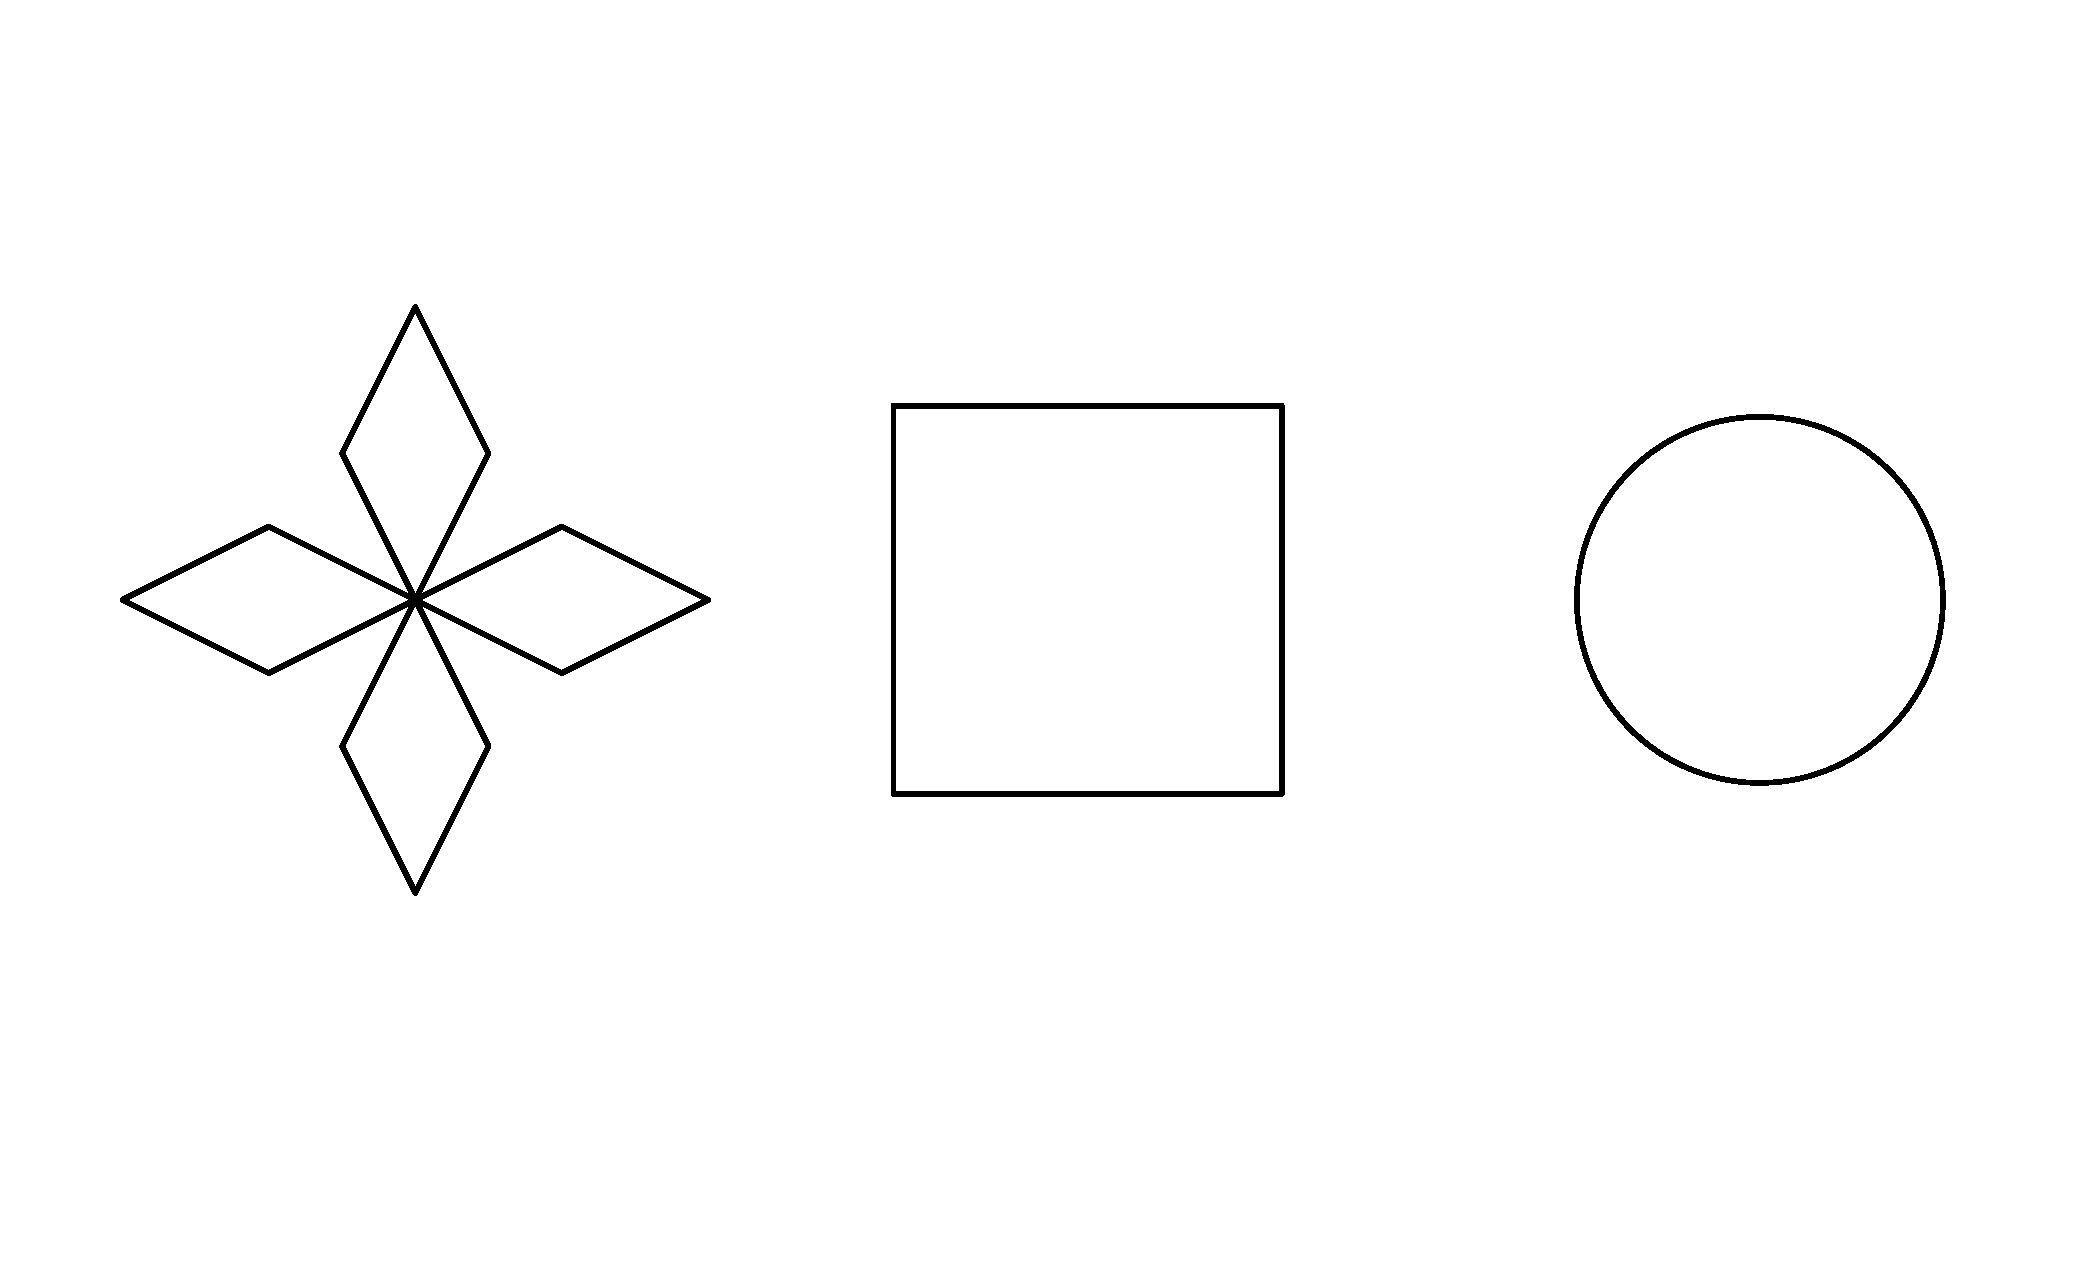
\includegraphics[width=.7\linewidth]{img/shape.pdf}
			
			Size
			
			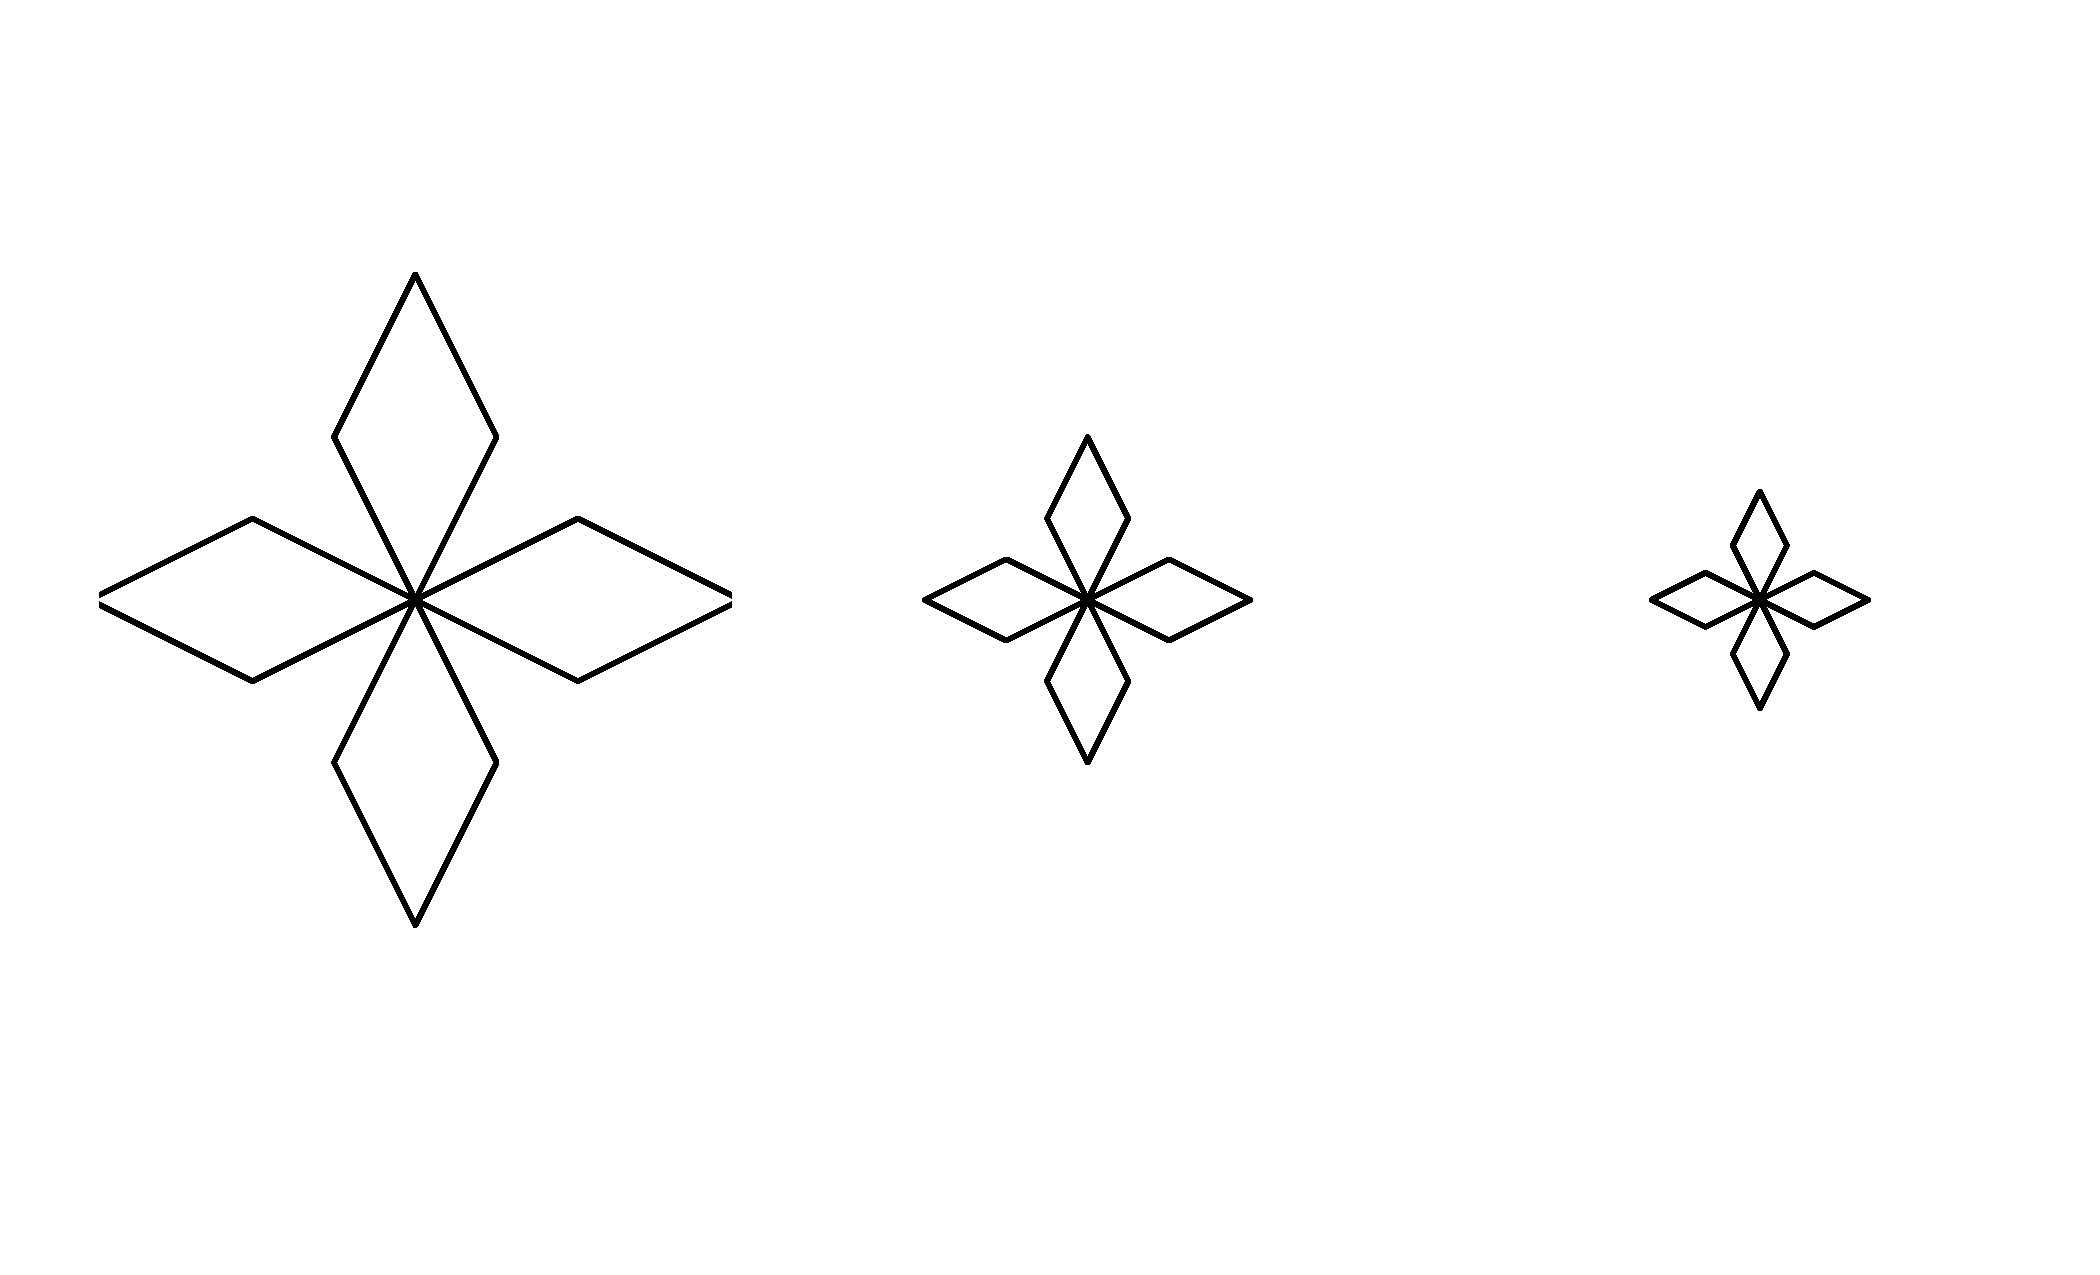
\includegraphics[width=.7\linewidth]{img/size.pdf}
		\end{column}
	\end{columns}
	
	\vspace{5mm}
	\centering
	\Large
	
	$\ldots$
	
\end{frame}

\begin{frame}{Logical rules}
	\begin{columns}[T]
		\begin{column}{.50\linewidth}
			\centering
			AND ($\cap$)
			
			\includegraphics[width=.7\linewidth]{img/and.pdf}
		\end{column}
		
		\begin{column}{.50\linewidth}
			\centering
			OR ($\cup$)
			
			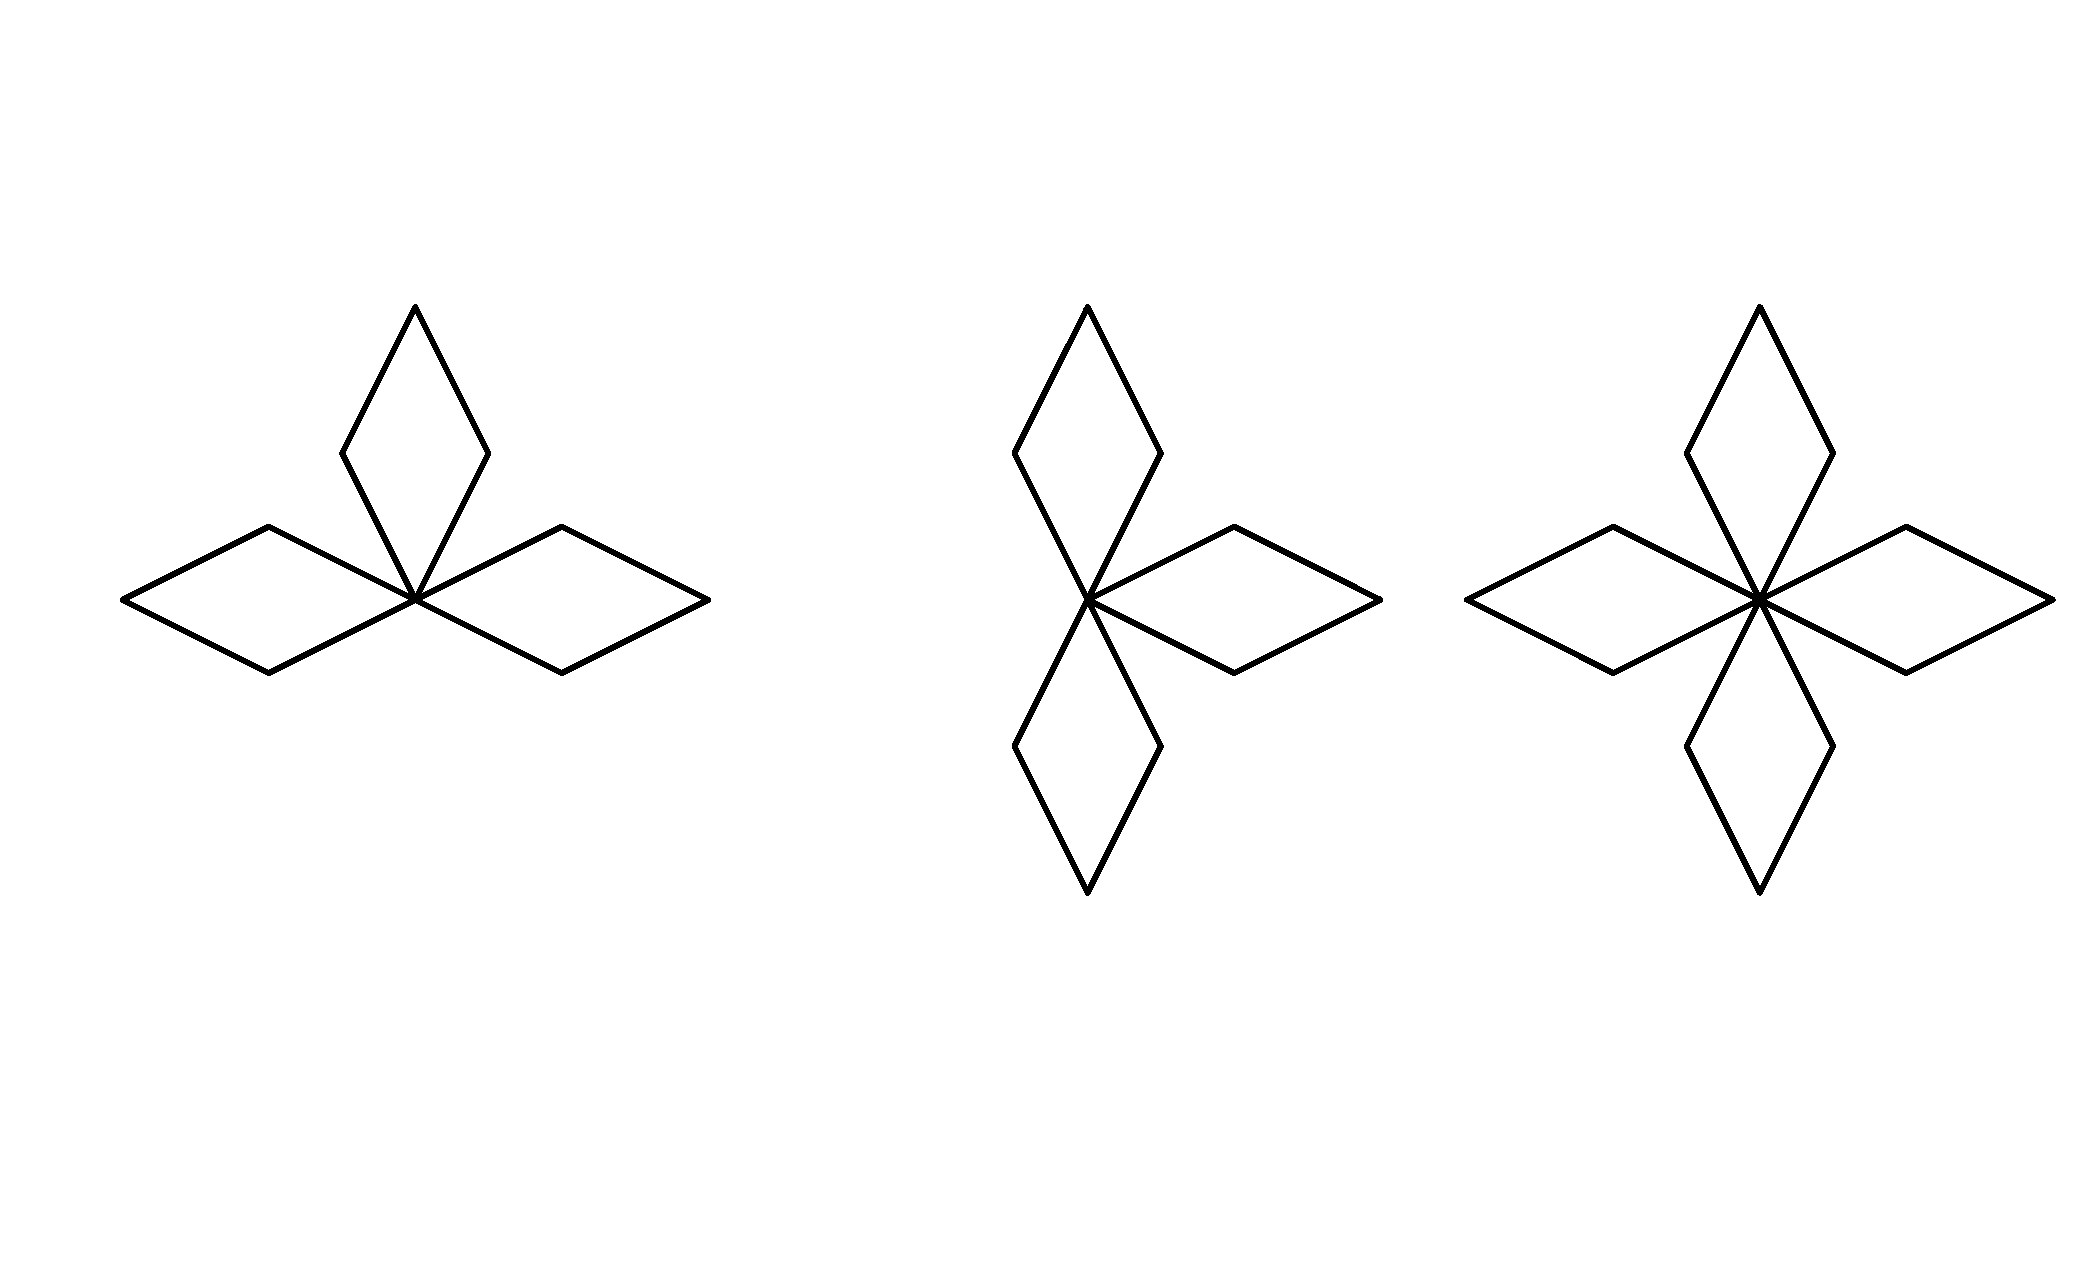
\includegraphics[width=.7\linewidth]{img/or.pdf}
		\end{column}
	\end{columns}
	
	\vspace{1.5mm}
	\centering
	
	XOR ($\Delta$)
	
	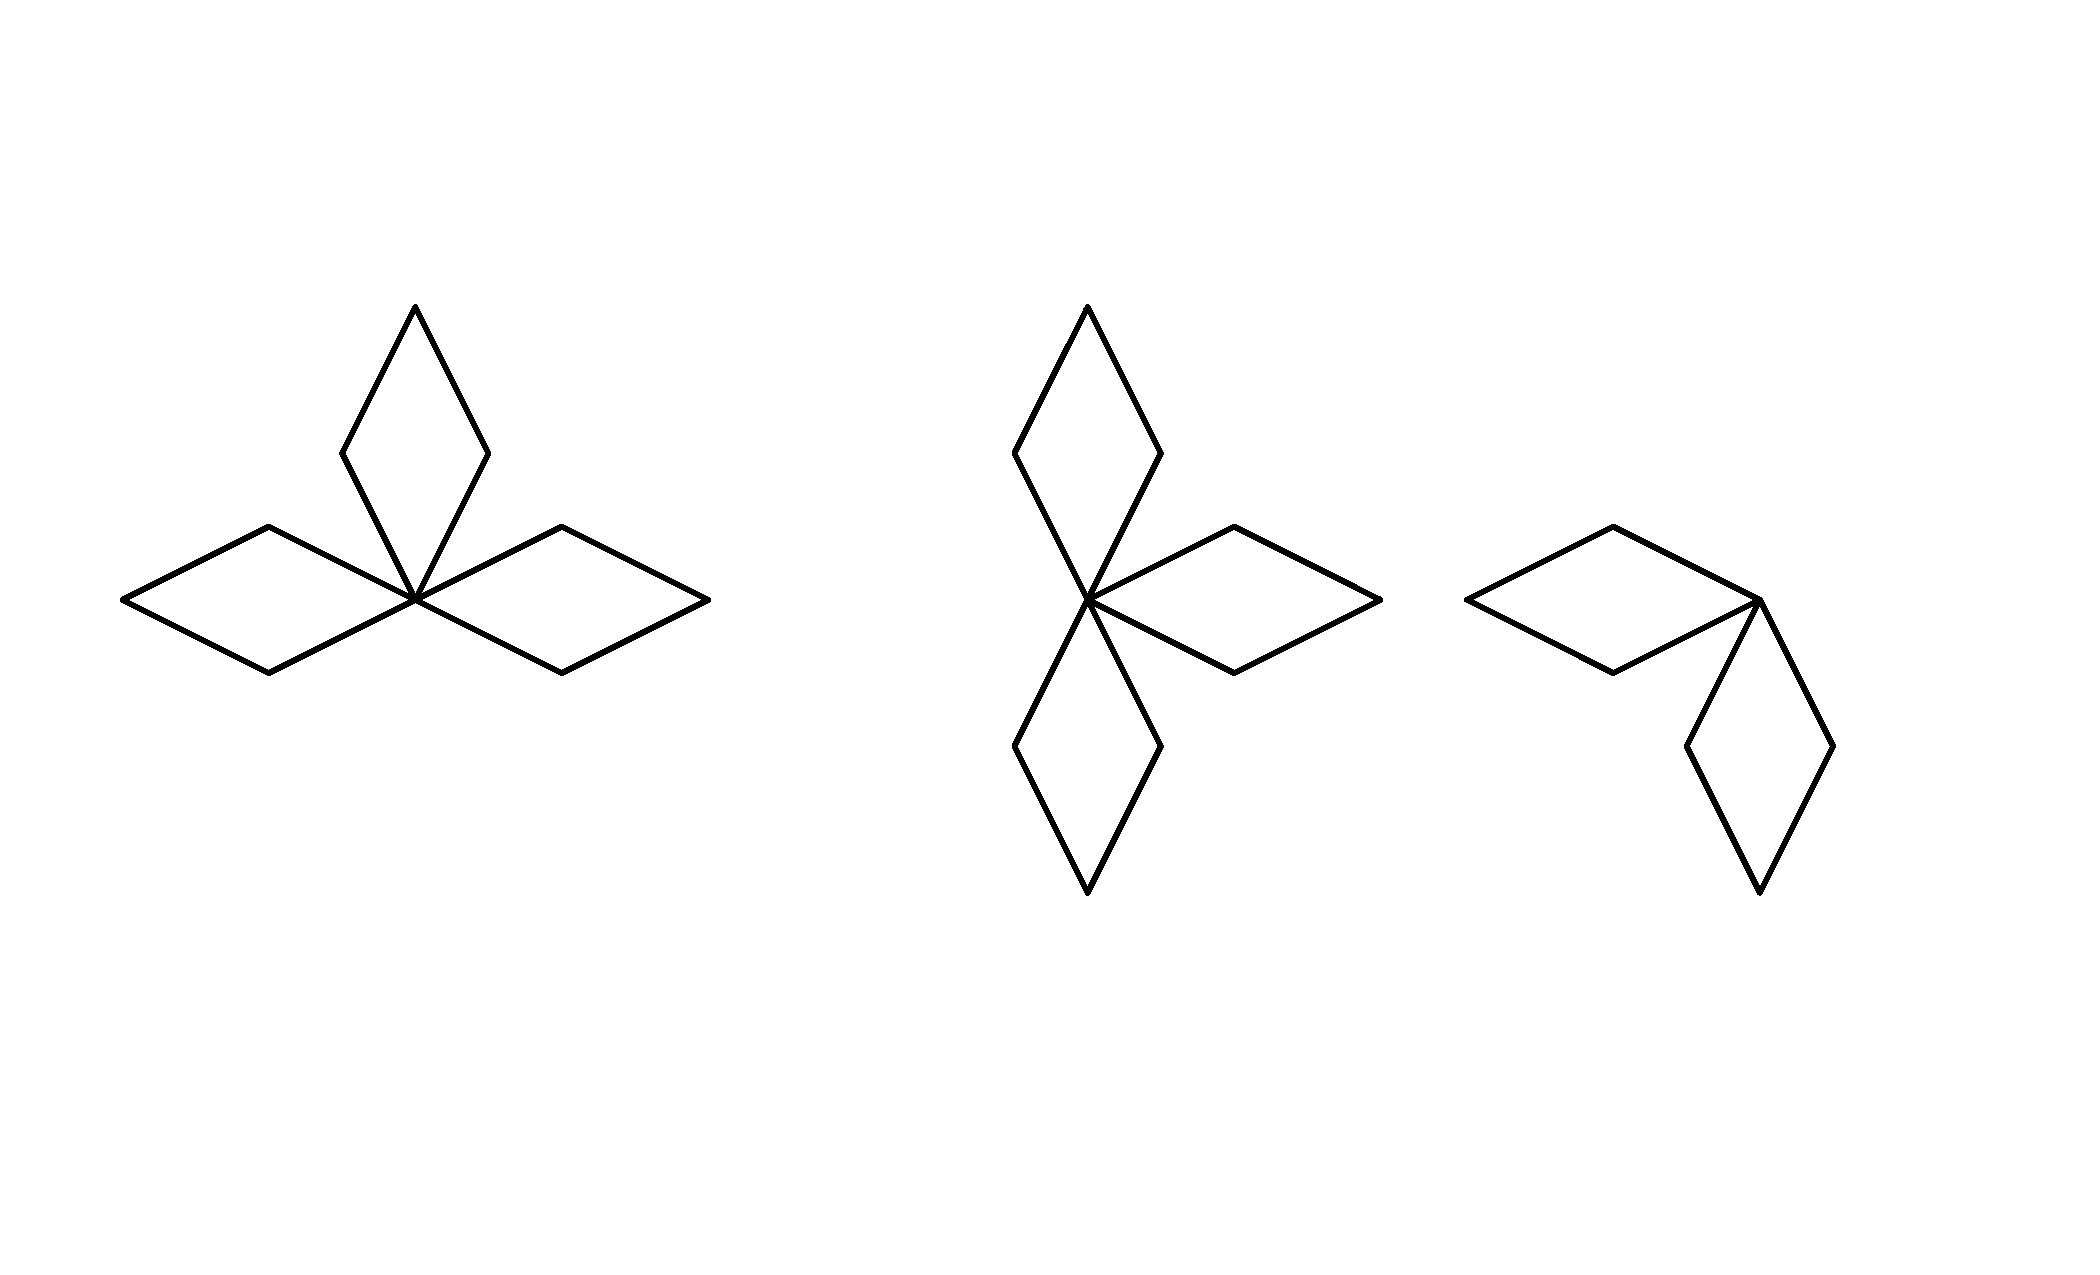
\includegraphics[width=.5\linewidth]{img/xor.pdf}
	
\end{frame}

\begin{frame}{Matriks generator}
	


		\begin{figure}
		\begin{tikzpicture}[node distance=1.5cm]
			\onslide<3->
			\node (start) [startstop] {Matrix generator};
			\node [xshift =+0.1cm, text width=4cm,font=\footnotesize, below of = start]
			{
			\centering	Directional logic: \\ Horizontal, vertical, diagonal
			};
			\onslide<1->
			\node (ob) [process, left of = start, yshift=1.5cm, xshift = -2cm] {Rule};
			\onslide<2->
			\node (rule) [process, left of = start, yshift=-1.5cm, xshift = -2cm] {Object};
			\onslide<4->
			\node (matrix) [rectangle ,right of = start, xshift = 3cm] {%
				\begin{tabular}{p{0.8cm} p{0.8cm} p{0.8cm}}
					Cell1 & Cell2 & Cell3  \\
					Cell4 & Cell5 & Cell6  \\
					Cell7 & Cell8 & \multicolumn{1}{c}{?} \\
			\end{tabular}};
			\onslide<3->	\path [->, shorten >= +3pt] (ob.east) edge (start.west);
			\onslide<3-> \path [->, shorten >= +3pt] (rule.east) edge (start.west);
			\onslide<4-> \path [->] (start.east) edge (matrix.west);
		\end{tikzpicture}
	\end{figure}
%	\onslide<2->
%\PutAt{(4.5cm,6cm)}{
%	\NormalBox[text width=4cm, font=\footnotesize]{Directional logic: \\ horizontal, vertical, diagonal}
%}
\end{frame}





\begin{frame}{}
	
	\begin{figure}
		\begin{tikzpicture}[node distance=1.5cm]
			\onslide<3->
			\node (start) [startstop] {\texttt{mat\_apply()}};
					\node [text width=4cm,font=\footnotesize, below of = start]
			{
				Directional logic:  \centering \\ Horizontal \\
			};
			\onslide<1->
			\node (ob) [process, left of = start, yshift=1.5cm, xshift = -2cm] {\texttt{rotate}};
			\onslide<2->
			\node (rule) [process, left of = start, yshift=-1.5cm, xshift = -2cm] {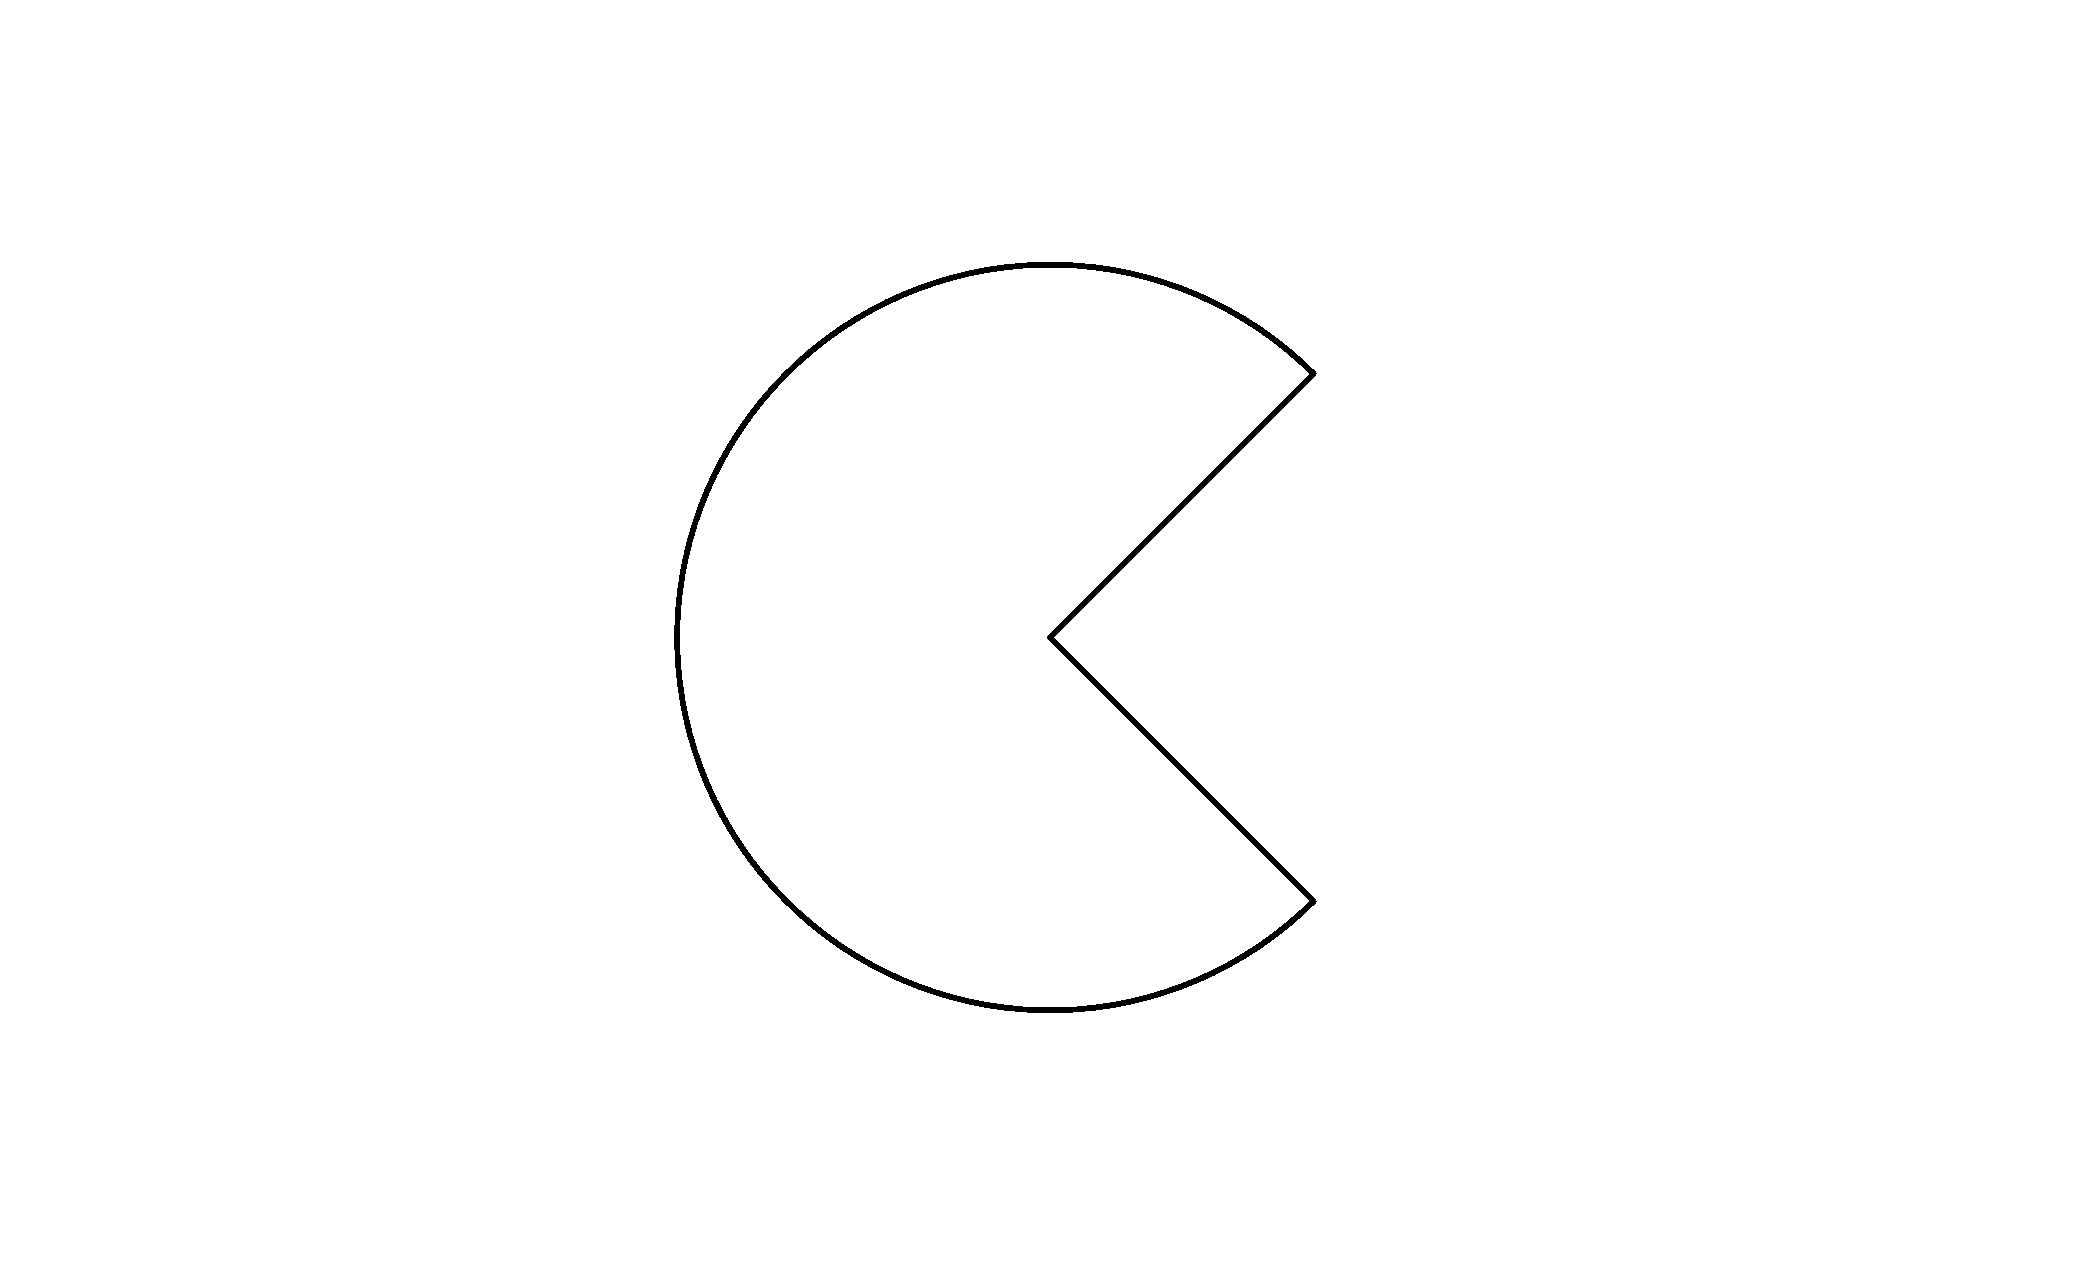
\includegraphics[width=\linewidth]{img/pacman.pdf}};
			\onslide<4->
			\node (matrix) [rectangle ,right of = start, xshift = 3cm] {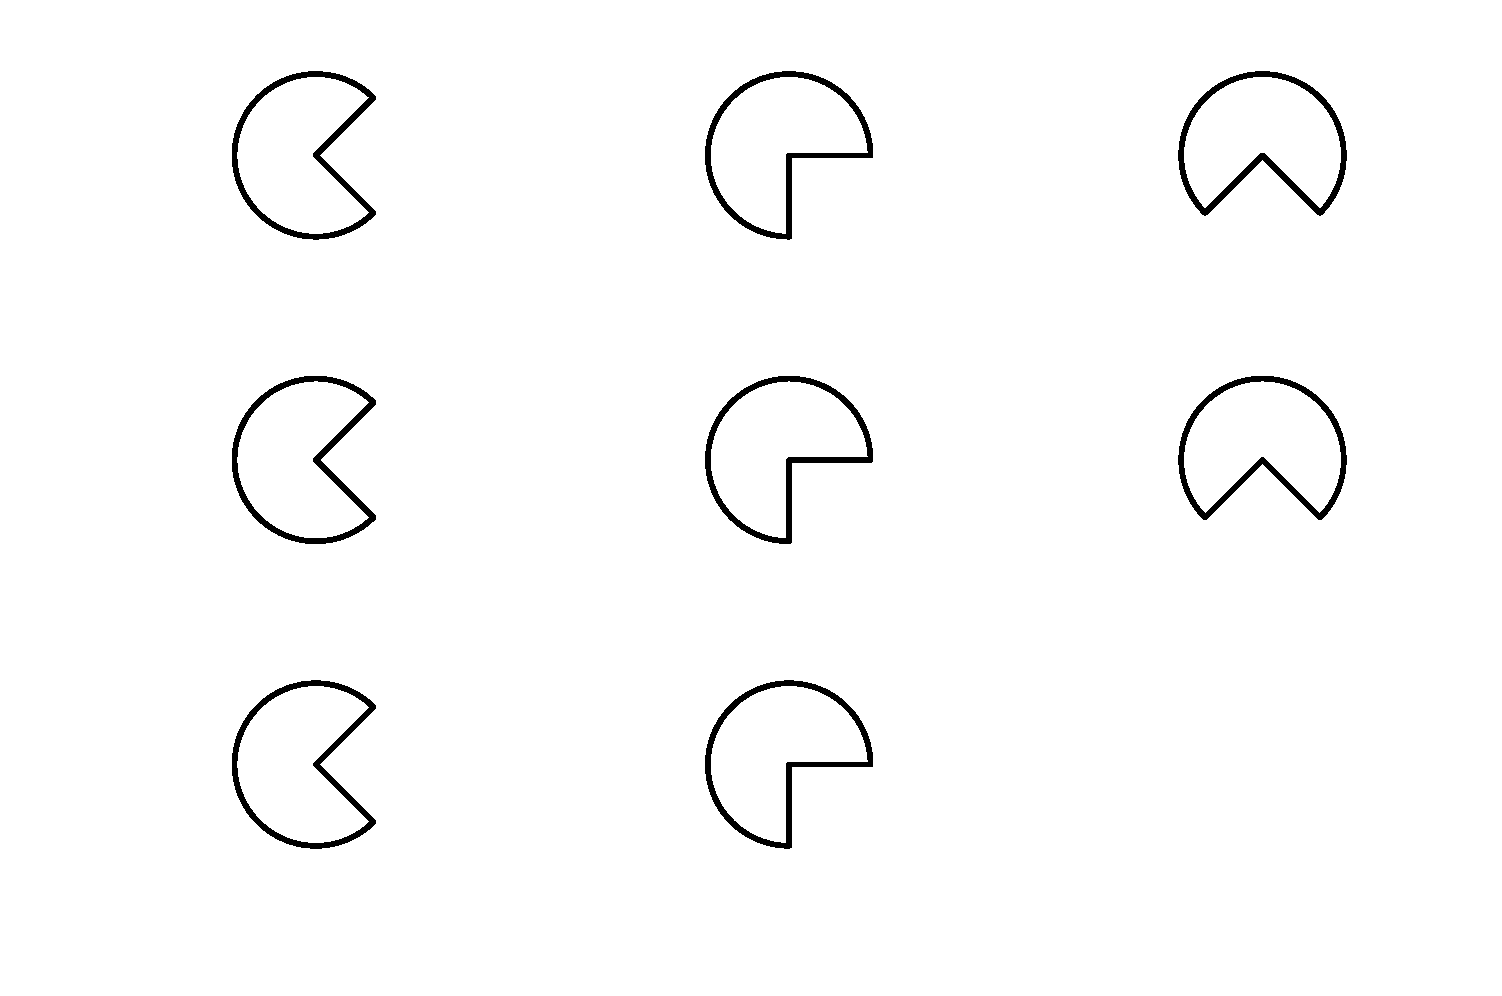
\includegraphics[width=.40\linewidth]{img/pacmanMatrix.pdf}};
			\onslide<3->	\path [->, shorten >= +3pt] (ob.east) edge (start.west);
			\onslide<3-> \path [->, shorten >= +3pt] (rule.east) edge (start.west);
			\onslide<4-> \path [->] (start.east) edge (matrix.west);
		\end{tikzpicture}
	\end{figure}
\end{frame}



\begin{frame}{Response options generator}
	

		
		\begin{tikzpicture}[node distance=2cm]
							\onslide<2->
%			\node[startstop] at (0, 0)   (start) {Response options generator};
	\node[startstop] at (0, 1)   (start) {Response options generator};
			\onslide<1->
			\node (matrix) [rectangle ,above of = start] {%
				\begin{tabular}{p{0.8cm} p{0.8cm} p{0.8cm}}
					Cell1 & Cell2 & Cell3  \\
					Cell4 & Cell5 & Cell6  \\
					Cell7 & Cell8 & \multicolumn{1}{c}{?}  \\
					\end{tabular}};
		\onslide<3->
		\node (response) [xshift =+4cm, text width=6cm,font=\large, right of = start]
		{  
			\centering
			\begin{tabular}{p{4cm}p{1cm}}
		\multicolumn{1}{c}{\textcolor{myGreen}{Correct}}		& $\times 1$  \\
			\multicolumn{1}{c}{\textcolor{repetition}{ Repetition}} & $\times 3$  \\
			\multicolumn{1}{c}{\textcolor{ic}{ Incomplete Correlate}} & $\times 4$  \\
					
		\multicolumn{1}{c}{	\textcolor{wp}{Wrong Principle} } &$\times 2$  \\
	\multicolumn{1}{c}{	\textcolor{difference}{Difference}} & $\times 1$ \\ 
			\end{tabular}
%			\centering		\textcolor{myGreen}{Correct} \normalsize{ (1)}\\ \vspace{3mm} \textcolor{ic}{ Incomplete Correlate}  \normalsize{ (4)} \\ \vspace{3mm} \textcolor{wp}{Wrong Principle} \normalsize{ (2)} \\  \vspace{3mm} \textcolor{difference}{Difference} \normalsize{ (1)}\\
		};
					
			\onslide<2-> \path [->,shorten >= +3pt] (matrix.south) edge (start.north);
			\onslide<3-> \path [->, shorten >= +2pt] (start.east) edge (response.west);
		\end{tikzpicture}

\end{frame}


\begin{frame}{}
	
			\begin{tikzpicture}[node distance=3cm]
		\onslide<2->
		%			\node[startstop] at (0, 0)   (start) {Response options generator};
		\node[startstop] at (0, -3.5)   (start) {\texttt{response\_list()}};
		\onslide<1->
		\node (matrix) [rectangle ,above of = start] {%
				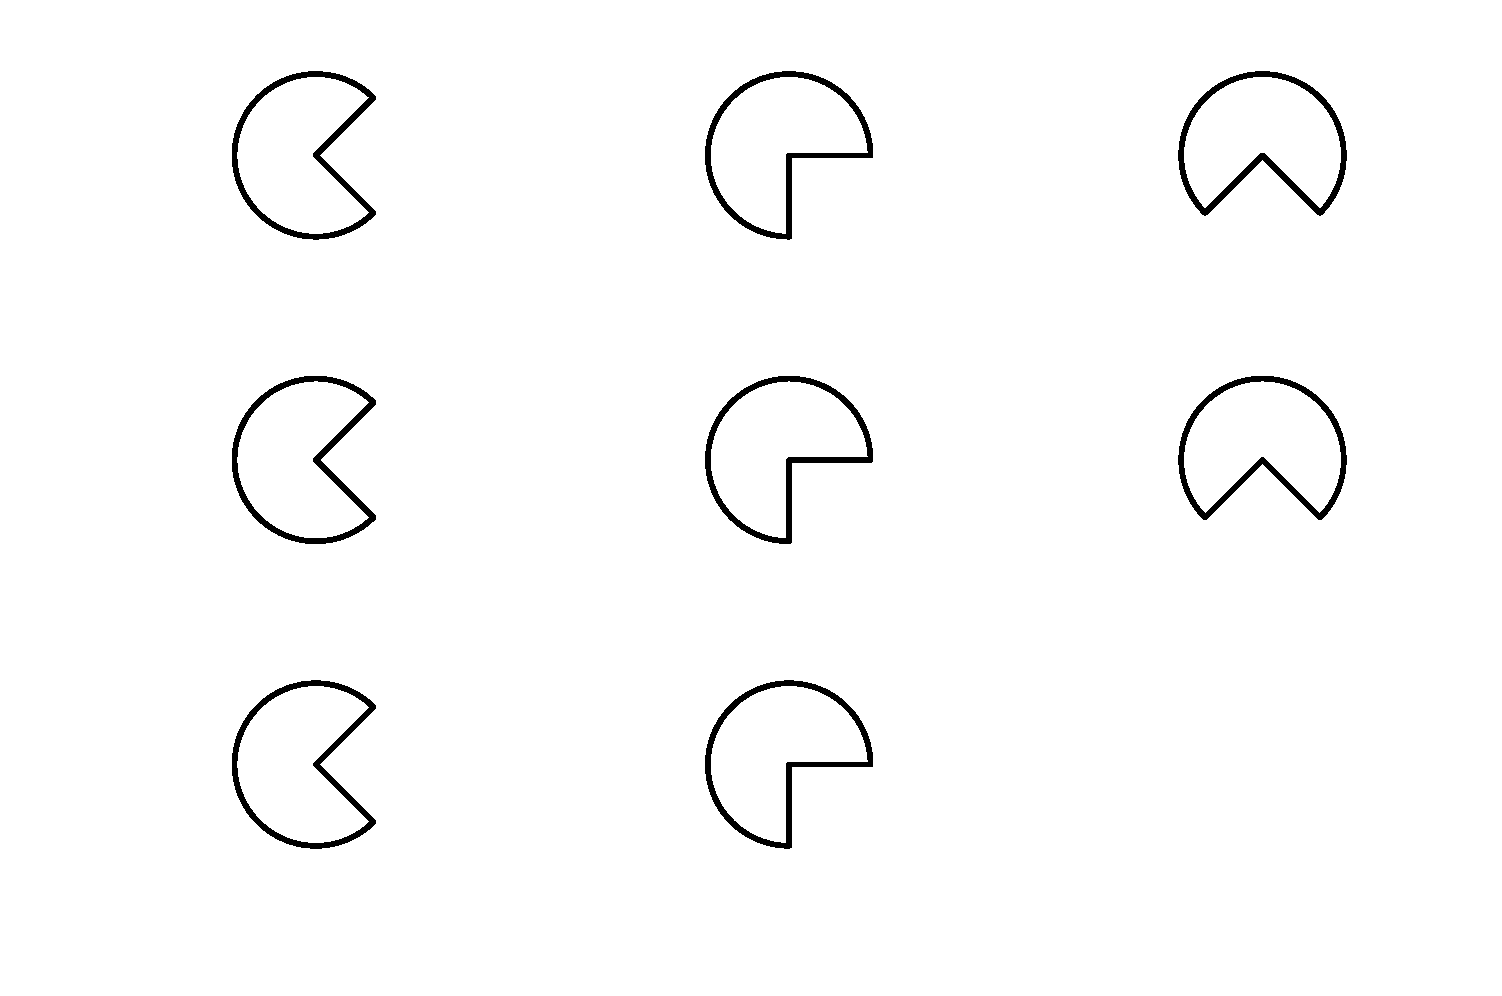
\includegraphics[width=.40\linewidth]{img/pacmanMatrix.pdf}
			};
		\onslide<3->
		\node (response) [xshift =+4cm, yshift=+2cm, text width=6cm,font=\large, right of = start]
		{  
			\centering
%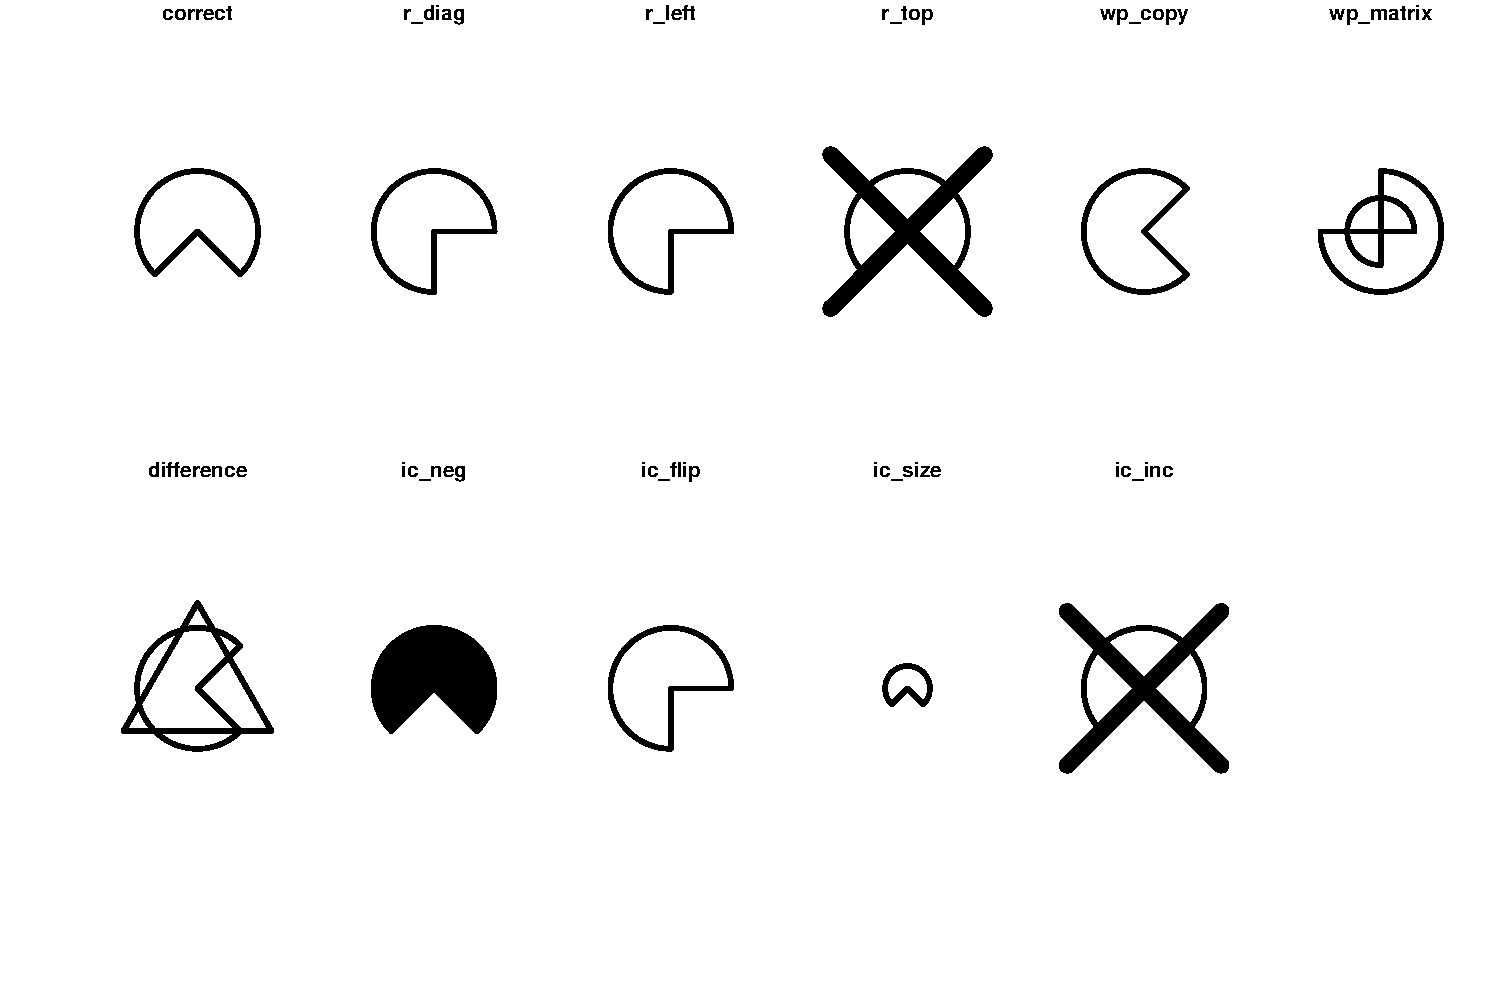
\includegraphics[width=\linewidth]{img/pacmanResponses.pdf}
\scalebox{.60}{
\begin{tabular}{c c }
\cellcolor{myGreen!70}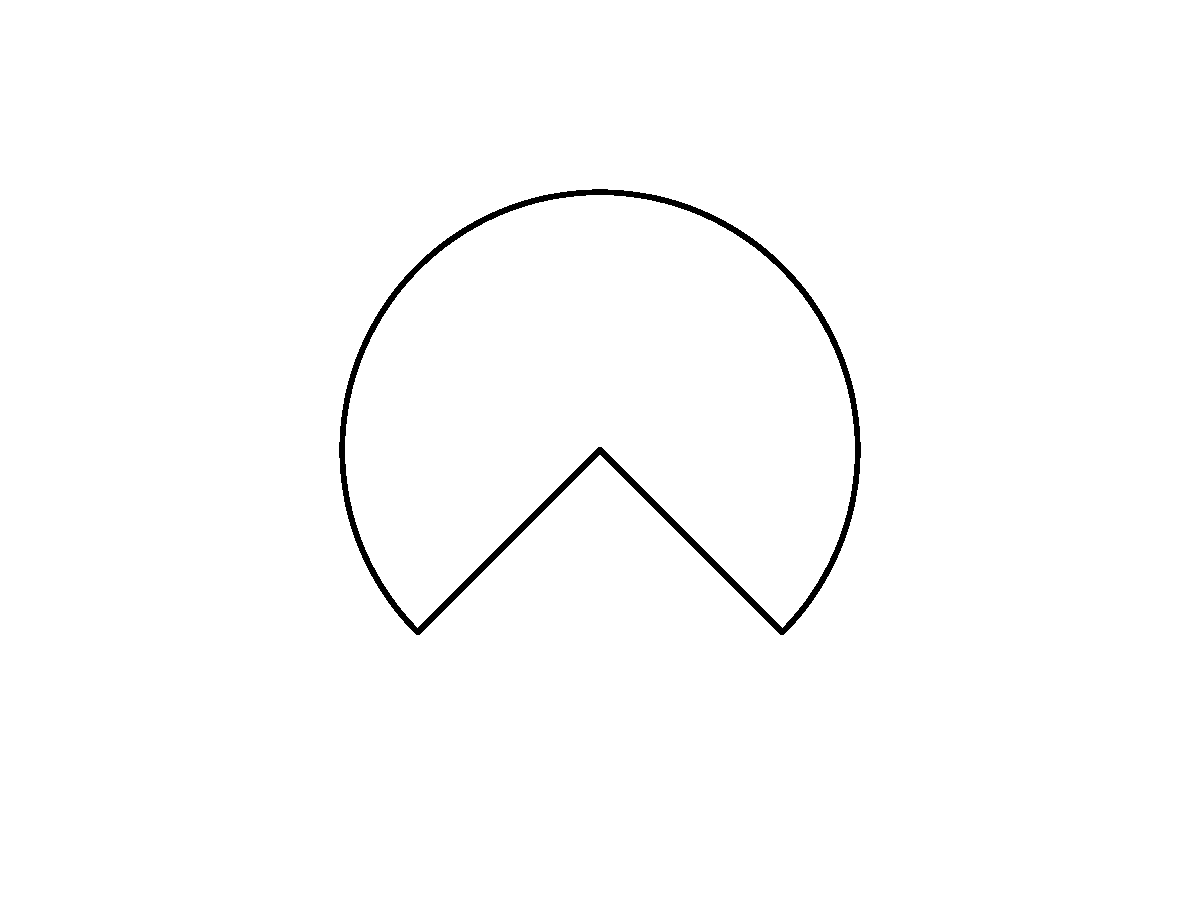
\includegraphics[width=.4\linewidth]{img/correct.pdf} &  \cellcolor{repetition!70}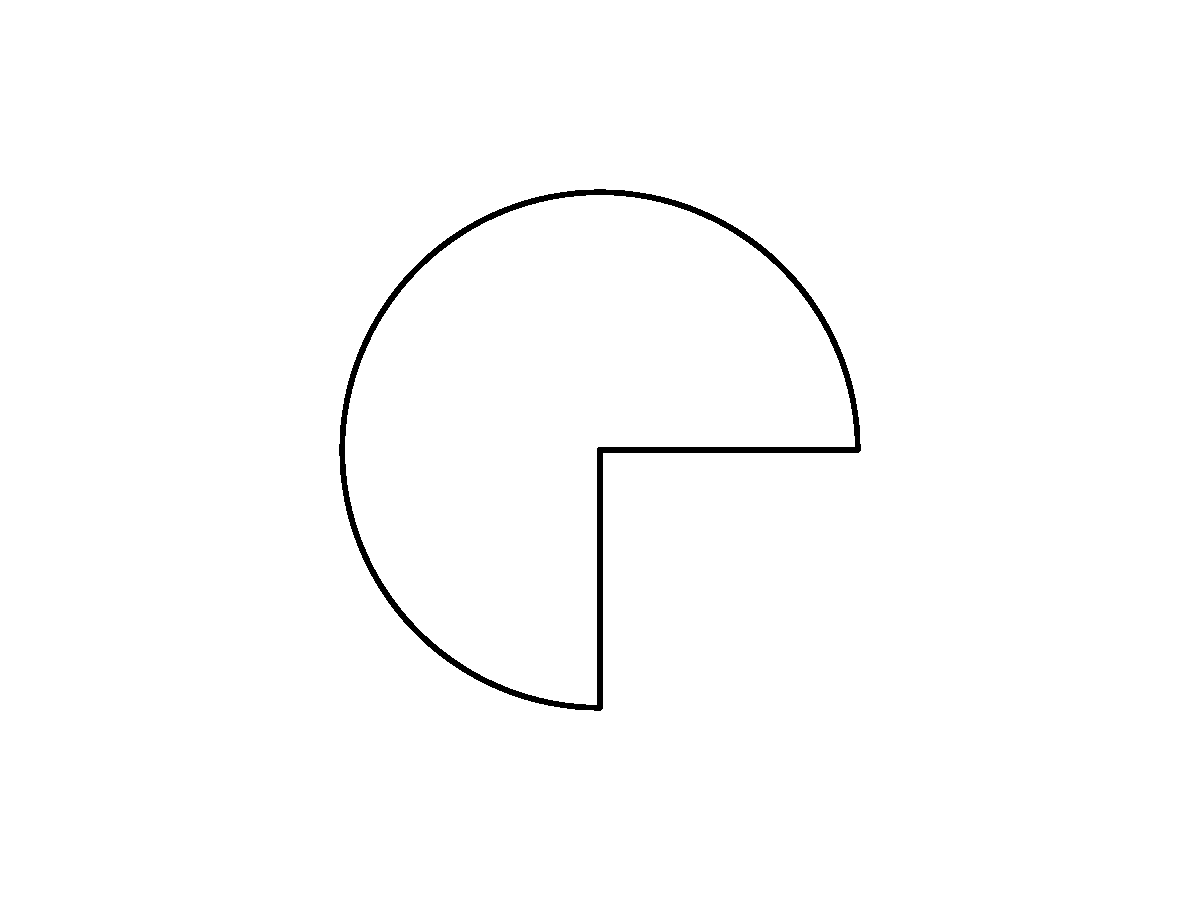
\includegraphics[width=.4\linewidth]{img/rleft.pdf}\\
\cellcolor{repetition!70}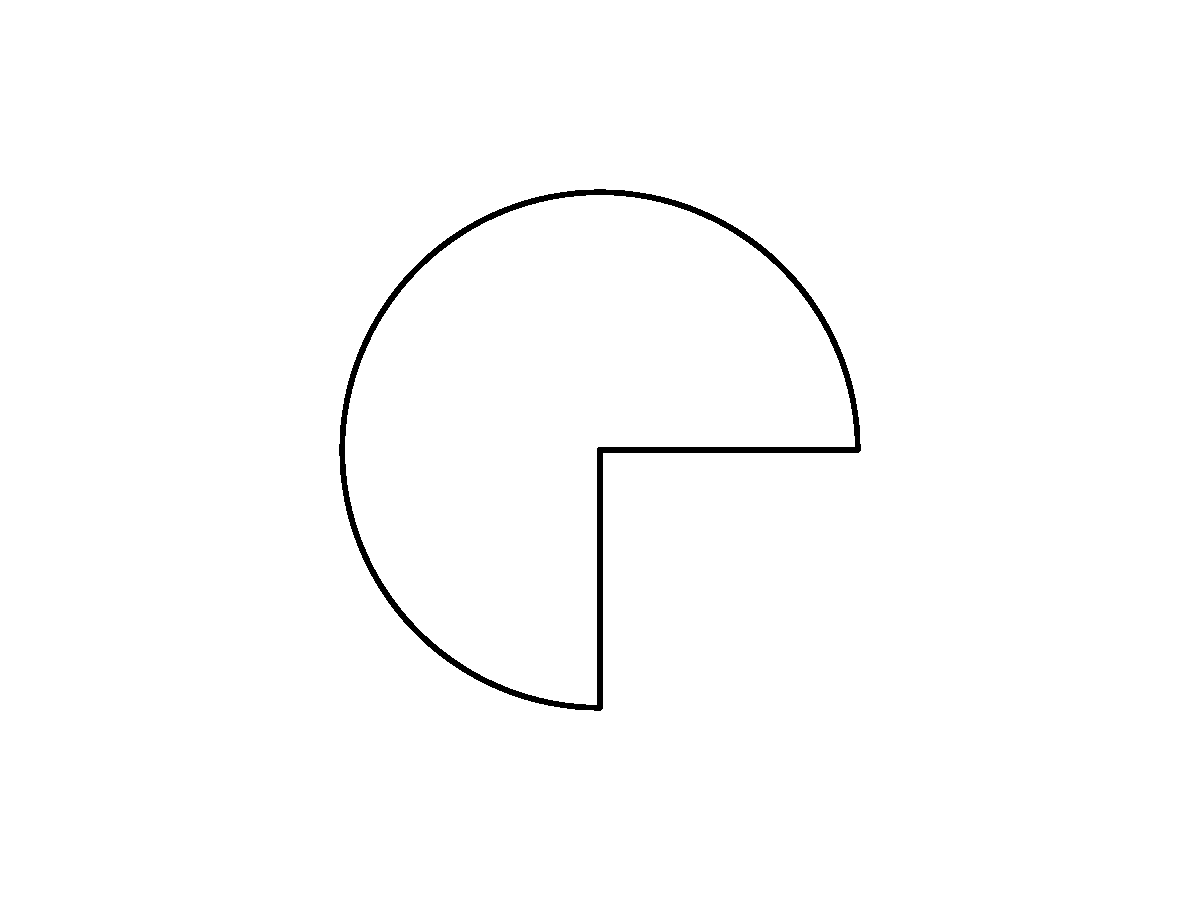
\includegraphics[width=.4\linewidth]{img/rdiag.pdf} & \cellcolor{repetition!70}
\includegraphics[width=.4\linewidth]{img/rtop.pdf}\\ 
\cellcolor{ic!70}	
\includegraphics[width=.4\linewidth]{img/icneg.pdf} &  \cellcolor{ic!70}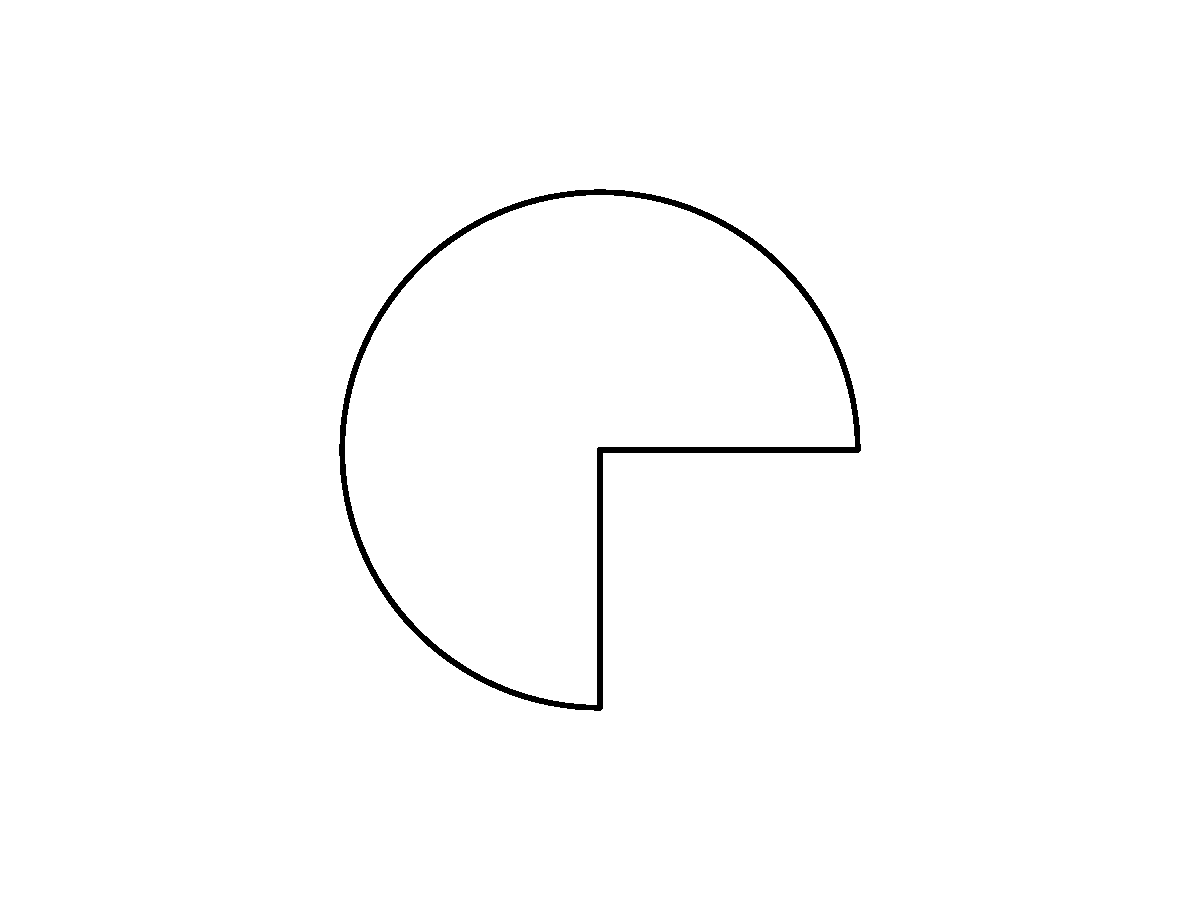
\includegraphics[width=.4\linewidth]{img/icflip.pdf} \\
\cellcolor{ic!70}	
\includegraphics[width=.4\linewidth]{img/icsize.pdf} &  \cellcolor{ic!70} 
\includegraphics[width=.4\linewidth]{img/icinc.pdf} \\
\cellcolor{wp!70}	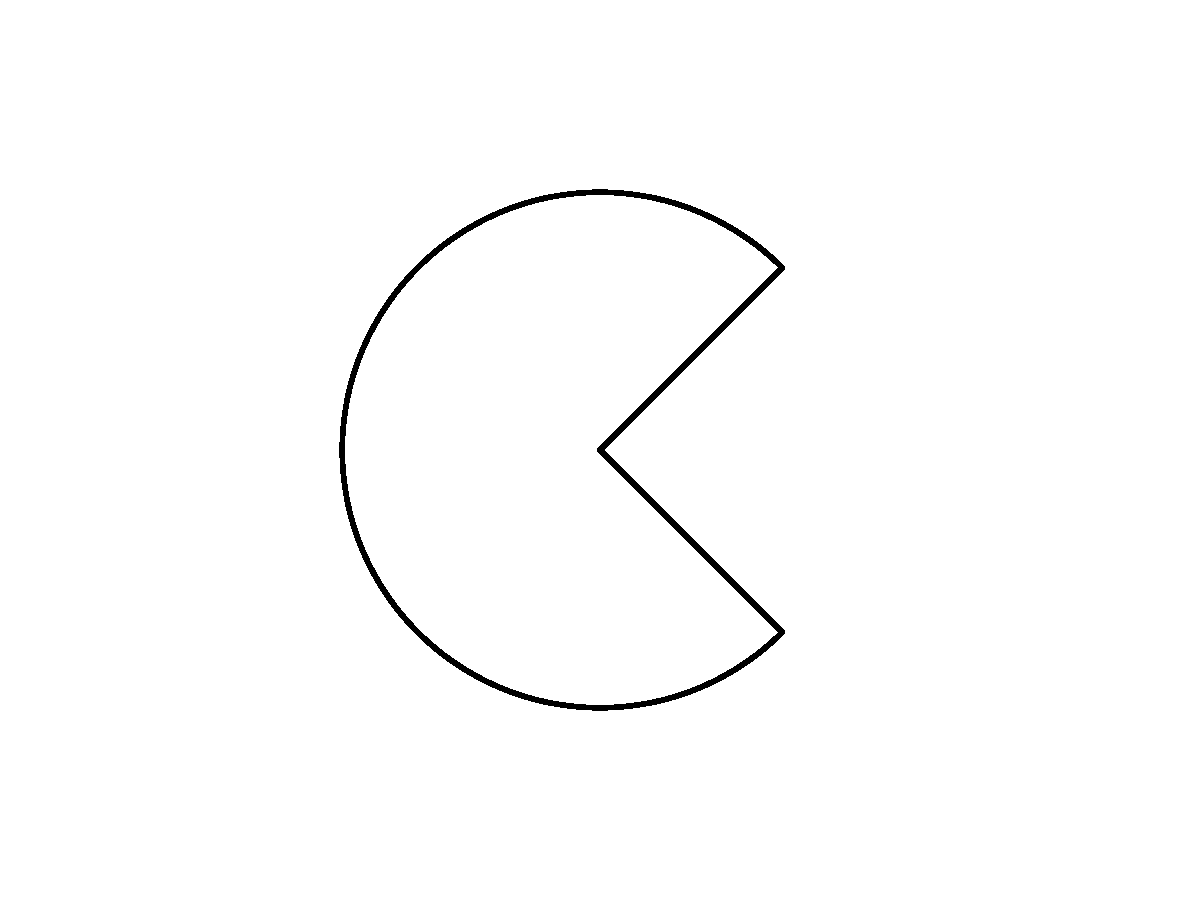
\includegraphics[width=.4\linewidth]{img/wpcopy.pdf} &  \cellcolor{wp!70} 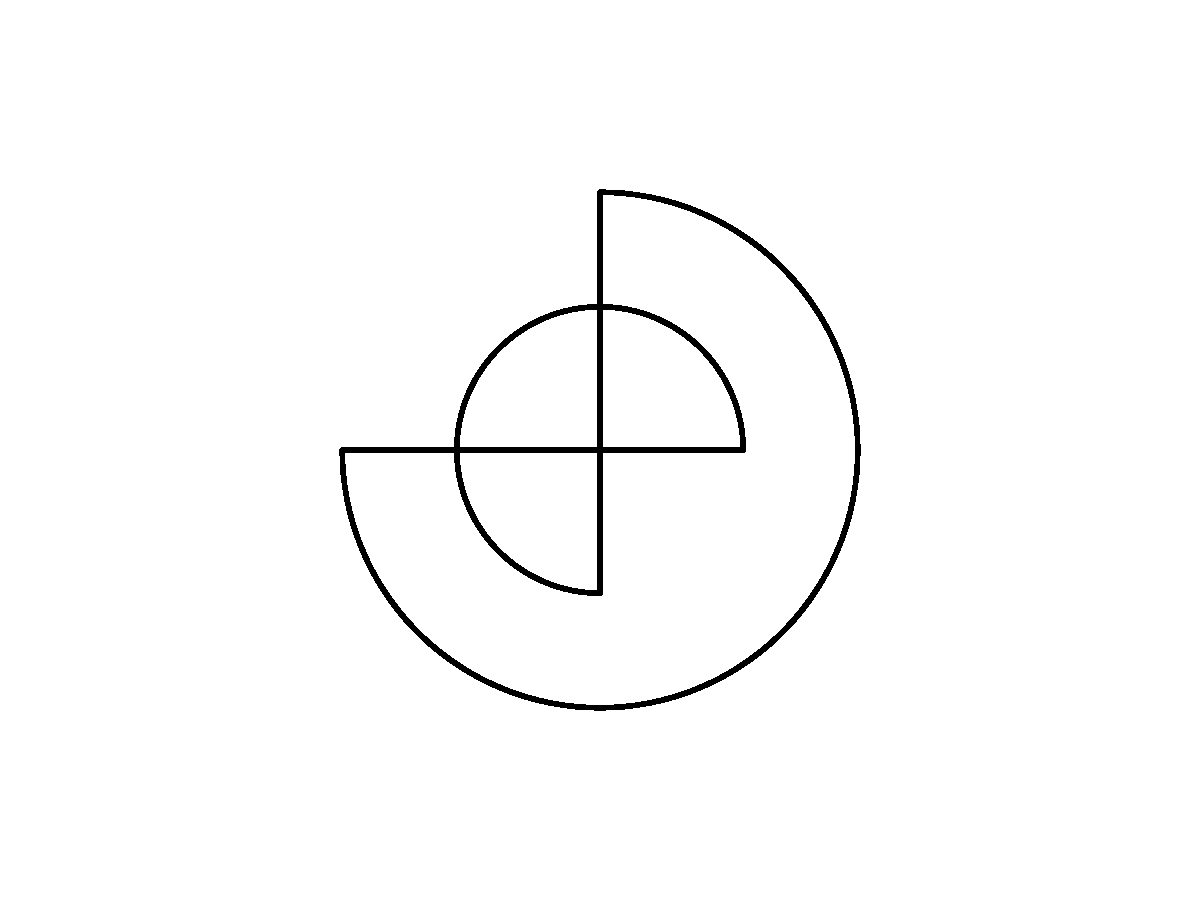
\includegraphics[width=.4\linewidth]{img/wpmatrix.pdf} \\
\cellcolor{difference!70}	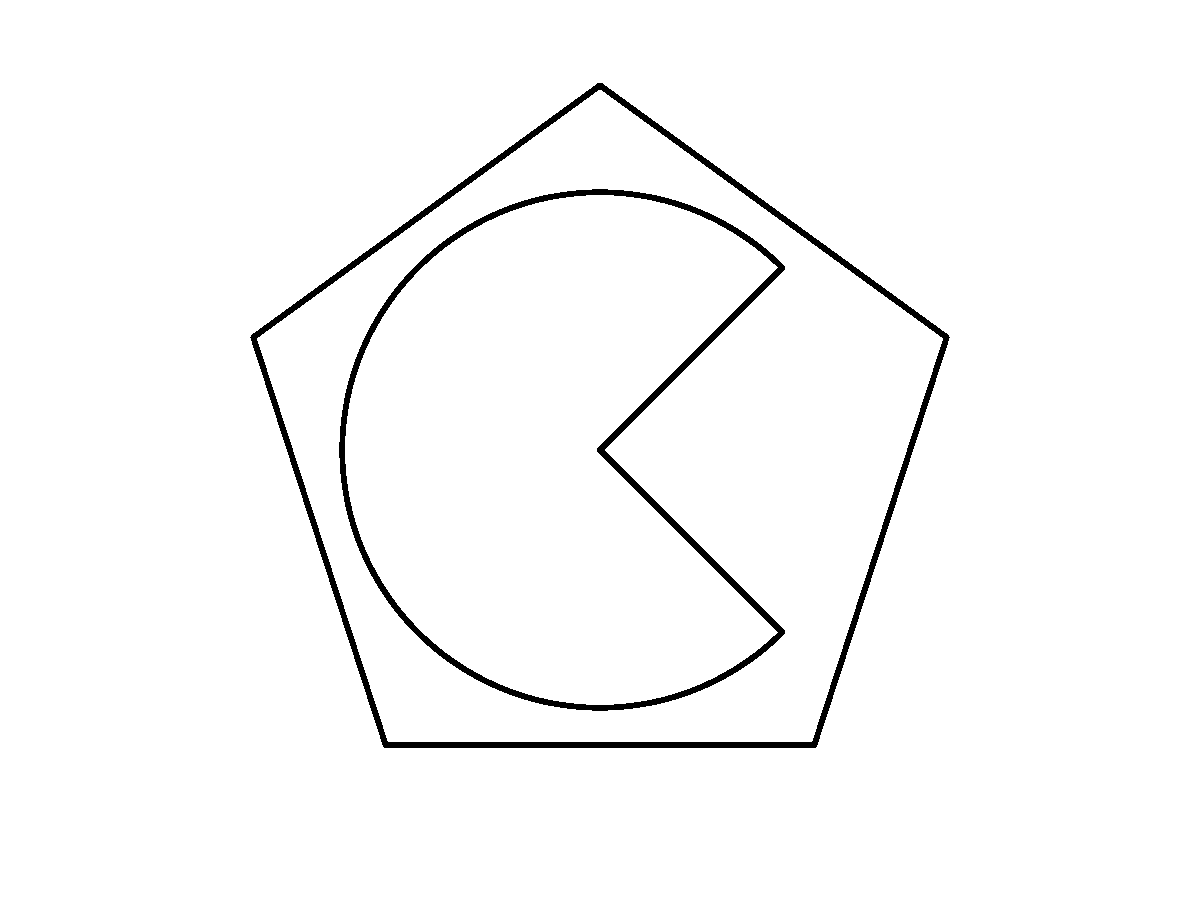
\includegraphics[width=.4\linewidth]{img/difference.pdf} & \\
\end{tabular}
}
		};
		
		\onslide<2-> \path [->,shorten >= +3pt] (matrix.south) edge (start.north);
		\onslide<3-> \path [->, shorten >= +2pt, shorten <= +2pt] (start.east) edge (response.west);
	\end{tikzpicture}
	
%	\begin{figure}
%		\begin{tikzpicture}[node distance=2.5cm]
%			\onslide<2->
%			\node (start) [startstop] {\texttt{response\_list()}};
%			\onslide<1->
%			\node (matrix) [rectangle ,above of = start] {%
%			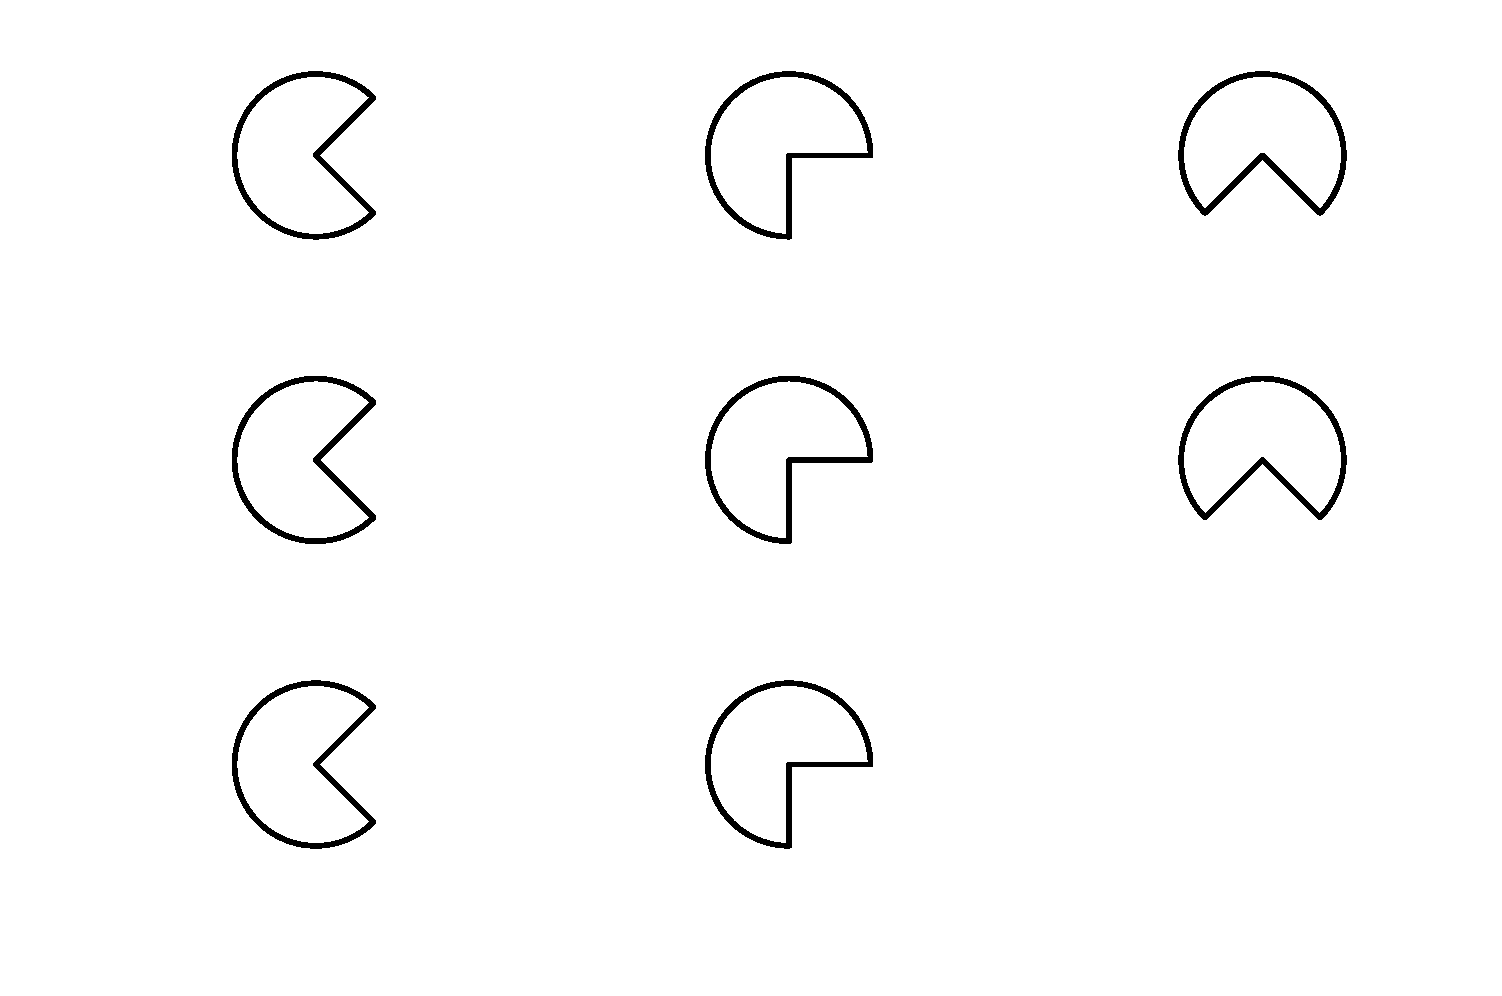
\includegraphics[width=.40\linewidth]{img/pacmanMatrix.pdf}
%				};
%			\onslide<3->
%			\node (response) [rectangle ,below of = start, yshift=-4] {%
%			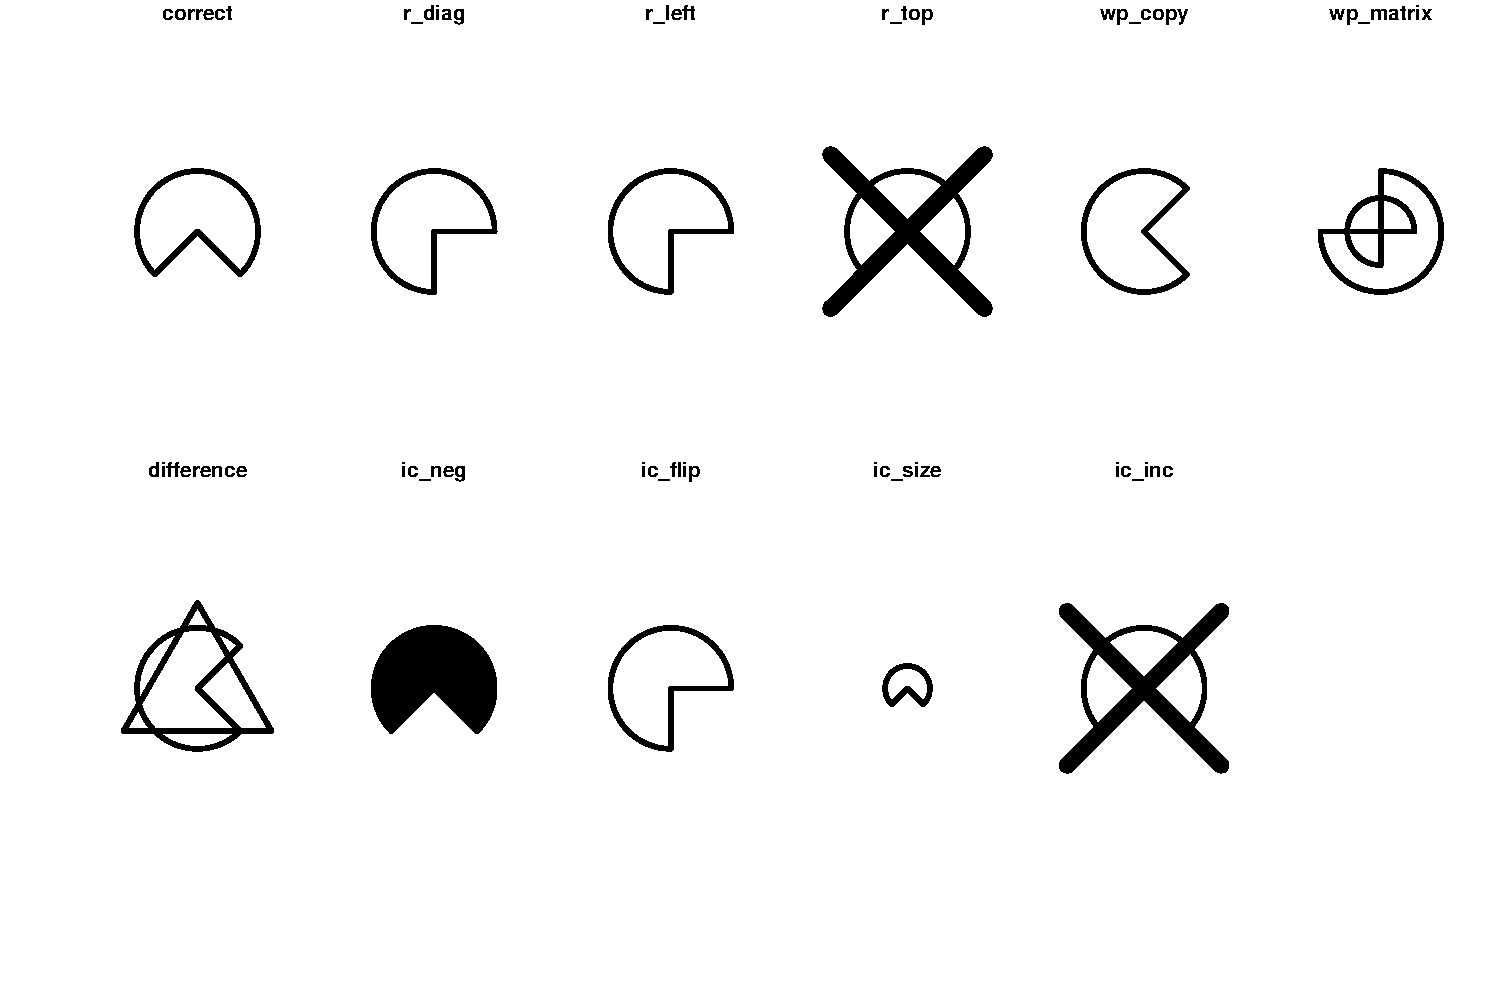
\includegraphics[width=.40\linewidth]{img/pacmanResponses.pdf}
%			};
%			\onslide<2-> \path [->] (matrix.south) edge (start.north);
%			\onslide<3-> \path [->] (start.south) edge (response.north);
%		\end{tikzpicture}
%	\end{figure}
\end{frame}



\section{Why?}
\begin{frame}{PsycAssist}
	\begin{figure}
		\centering
		
\includegraphics[width=\linewidth]{img/psyc}
	\end{figure}
	
\end{frame}


\begin{frame}
	
%	\vspace*{-3mm}
%	
%	\begin{figure}
%		\centering
%		
\includegraphics[width=.6\linewidth]{img/psyc.png}
%	\end{figure}
	
		\vspace{-3mm}
				\begin{exampleblock}{Stimuli}
				\footnotesize
				40 Raven-like matrices: 
				
				\begin{itemize}
					\item $1 \times 1$ matrices (jigsaw puzzle) , \small{$n = 5$}
					\item $2 \times 2$ matrices, \small{$n = 20$}
					\item $3 \times 3$ matrices, \small{$n = 15$}
				\end{itemize}
				
			\end{exampleblock}
		
	
		\vspace{-2mm}
		
			\begin{exampleblock}{Sample}
			
			\footnotesize
			$n = 600$ children aged 4-11 ($M = 8.39\pm 2.17$), recruited in Italian schools 
			
			$F = 48$\%
			
			$30$\% preschoolers
			
		\end{exampleblock}

			\begin{exampleblock}{Rasch validation}
			
			\begin{itemize}
				\item Monotonicity check
				
				\item Fit the Rasch model: 
				
				\begin{enumerate}
					\item Check for item with infit and/or outfit statistics $\geq 2$ (underfit)
					\item Local dependence (Yeun's $Q3 \geq .20$)
				\end{enumerate}
			\end{itemize}
			
		\end{exampleblock}
			
	
	
\end{frame}

\begin{frame}{Rasch validation}
	\small

	
	\begin{block}{Note}
		
		\small
		2 matrices were eliminated because of technical issues 
		
		4 matrices were eliminated because of a lack of monotonicity 
	
	\end{block}

	
		The starting model included 34 matrices: 
	
\begin{center}
			\begin{tabular}[t]{c cc cc}
		\hline
		Madcov & SRMR & $p$-value\\
		\hline
		0.95 & 0.06 &   $0.001$\\
		\hline
	\end{tabular}
\end{center}


	Oufit statistic suggested the underfit of one matrix (item 21) $\rightarrow$ removed and refitted the model 
	
	
	\begin{itemize}
		\item Check for infit/outfit $\rightarrow$ no matrices were identified as underfitting
		\item Check for local dependence: 
		
		\begin{itemize}
			\item Matrix $37 - 40$ 
			\item Matrix $37 -  28$ 
			 \hspace{3mm}\makebox(0,0){\put(0,2.0\normalbaselineskip){%
					$\left. \rule{0pt}{1.1\normalbaselineskip}\right\}$ \scriptsize{$\rightarrow$ Matrix 37 has been eliminated}}}
		\end{itemize}
	\end{itemize}
\end{frame}

\begin{frame}{The final model}

\begin{table}
	\vspace*{-2mm}
	\centering
	\begin{tabular}[t]{ccccc}
		\hline
			Madcov & SRMR & $p$-value\\
		\hline
		0.94 & 0.06 & $ 0.001$\\
		\hline
	\end{tabular}
\end{table}


\begin{figure}
\centering

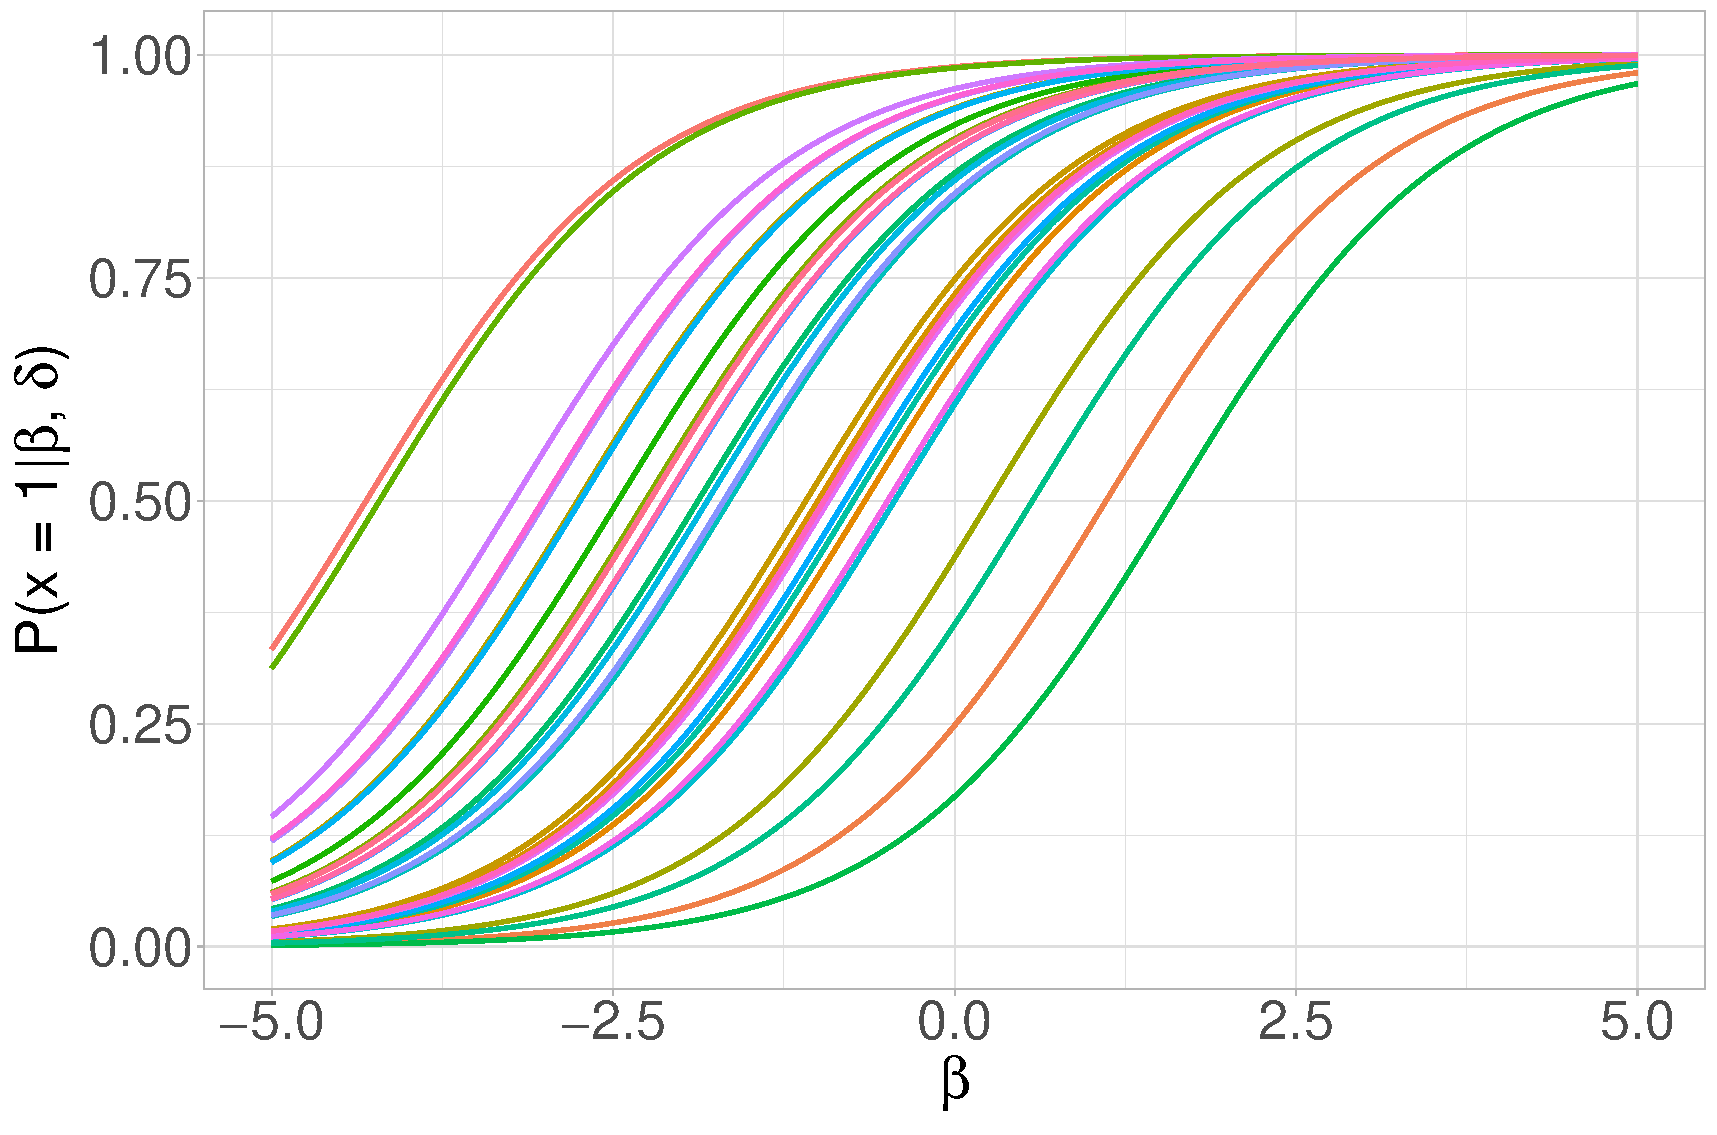
\includegraphics[width=.7\linewidth]{img/icc.pdf}
\end{figure}
	
\end{frame}

\section{Final remarks}

\begin{frame}
	\begin{itemize}
				\item Formalization of the matrix generation process
		
		\item Generate similar but different matrices $\rightarrow$  Equivalent matrices (?) 
		

		
		\item Reproducibility of the stimuli
		
		\item Ease of use (for use\texttt{R})
		
		\pause
		\vspace{2mm}
		\item[{\small
\includegraphics[height=2.4ex]{img/soon.png}}] A shiny app
	\end{itemize}
	
\end{frame}

\begin{frame}[plain]
			
			\centering
			
			\large mat\texttt{R}iks
			
			\vspace{3mm}
			
\includegraphics[width=.6\linewidth]{img/matriks.png}
			
			\footnotesize
			\href{https://github.com/OttaviaE/matRiks}{https://github.com/OttaviaE/matRiks}
		
		
	\onslide<2->
	
	\vspace{8mm}
	\centering
	
	\Large
	Thank you!
	\normalsize
	
	\vspace{3mm}
	ottavia.epifania@unipd.it
	
	

	\onslide<2->
		\begin{textblock*}{2cm}(10cm,8cm)
				\onslide<2->
		\includegraphics[width =\linewidth]{img/user.png}
	\end{textblock*}
	
\end{frame}

\end{document}
